% KDD AI4Sciences submissions are single-blind. Keep review mode, but list
% author names and affiliations.
\PassOptionsToPackage{table}{xcolor}
\documentclass[sigconf,review,balance=false]{acmart}
\citestyle{acmnumeric}
\setcopyright{none}
\settopmatter{printacmref=false, printccs=false, printfolios=true}
\renewcommand\footnotetextcopyrightpermission[1]{}
\acmConference[KDD '27]{Proceedings of the ACM SIGKDD Conference on Knowledge Discovery and Data Mining}{August 1--5, 2027}{San Jose, CA, USA}
\acmBooktitle{Proceedings of the ACM SIGKDD Conference on Knowledge Discovery and Data Mining (KDD '27), August 1--5, 2027, San Jose, CA, USA}
\acmYear{2027}
\copyrightyear{2027}
\acmDOI{}
\acmISBN{}
\acmSubmissionID{REPLACE-WITH-SUBMISSION-ID}
\usepackage[T1]{fontenc}
\usepackage{booktabs}
\usepackage{amsmath}
\usepackage{amssymb}
\usepackage{amsfonts}
\usepackage{nicefrac}
\usepackage{array}
\usepackage{multirow}
\usepackage{makecell}
\usepackage{colortbl}
\usepackage{xspace}
\usepackage{tabularx}
\usepackage{algorithm}
\usepackage{algpseudocode}
\usepackage{placeins}
\usepackage[capitalize]{cleveref}
\setcitestyle{numbers,square,comma,sort&compress}
\graphicspath{{./}{appendix_image/}}
\crefname{section}{Sec.}{Secs.}
\Crefname{section}{Section}{Sections}
\crefname{table}{Tab.}{Tabs.}
\Crefname{table}{Table}{Tables}
\crefname{figure}{Fig.}{Figs.}
\Crefname{figure}{Figure}{Figures}
\crefname{equation}{Eq.}{Eqs.}
\Crefname{equation}{Equation}{Equations}
\setcounter{topnumber}{5}
\setcounter{bottomnumber}{5}
\setcounter{totalnumber}{10}
\renewcommand{\topfraction}{0.95}
\renewcommand{\bottomfraction}{0.95}
\renewcommand{\textfraction}{0.05}
\renewcommand{\floatpagefraction}{0.8}
\renewcommand{\dbltopfraction}{0.95}
\renewcommand{\dblfloatpagefraction}{0.8}
\setlength{\textfloatsep}{10pt plus 2pt minus 2pt}
\setlength{\floatsep}{8pt plus 2pt minus 2pt}
\setlength{\intextsep}{10pt plus 2pt minus 2pt}
% Paper macros.
\newcommand{\methodname}{\textsc{Spine}\xspace}
\newcommand{\ppp}{\textsc{PPP}\xspace}
\newcommand{\redadd}[1]{\textcolor{red}{#1}}
\newcommand{\redfill}[1]{\textcolor{red}{\textbf{[#1]}}}
\newcommand{\softpara}{\vspace{0.25em}}
\newcommand{\pmv}[2]{\ensuremath{#1\,{\scriptstyle\pm\,#2}}}

\title{\methodname{}: Single-Cell Spatial Perturbation-Field Inference in Niche Environments}




\author{Xi Li}
\email{xil43@uci.edu}
\affiliation{%
  \institution{University of California, Irvine}
  \city{Irvine}
  \state{California}
  \country{USA}
}
\author{Ziheng Duan}
\affiliation{%
  \institution{University of California, Irvine}
  \city{Irvine}
  \state{California}
  \country{USA}
}
\author{Simon Dongbo Sun}
\affiliation{%
  \institution{University of California, Irvine}
  \city{Irvine}
  \state{California}
  \country{USA}
}
\author{Martin Renqiang Min}
\affiliation{%
  \institution{NEC Laboratories America}
  \city{Princeton}
  \state{New Jersey}
  \country{USA}
}
\author{Yang Liu}
\affiliation{%
  \institution{Yale University}
  \city{New Haven}
  \state{Connecticut}
  \country{USA}
}
\author{Jing Zhang}
\affiliation{%
  \institution{University of California, Irvine}
  \city{Irvine}
  \state{California}
  \country{USA}
}
\raggedbottom
\begin{document}




\begin{abstract}
Spatial perturbation assays preserve tissue architecture, but observed neighbor
responses mix tissue context and perturbation effects.
We construct Pre--Post Perturbation Pairing (\ppp), an audited matched-control
pseudo-target benchmark, and \methodname{}, a predictive decomposition.
\methodname{} predicts the context component before modeling residuals from a
direct-effect profile and sender region. On a fully disjoint
1,342/837/928-graph train/validation/test split, \methodname{} increases pooled
Ring Pearson from 0.3626 to 0.4111; the mean graph-paired lift is $+0.0532$
(95\% CI, 0.0474--0.0586). Context-only and full models reach predictive
$R^2$ values of 0.3712 and 0.4669, corresponding to an incremental partial
$R^2$ of 0.1521 (0.1476--0.1559). Gene-disjoint and no-expression matching
retain positive Ring lift, but removing spatial matching eliminates it.
The signal therefore depends on spatially matched controls rather than
expression overlap alone. Factorial controls identify contributions from
direct-effect profile identity and sender location; randomized communication
scores have no measurable effect. Across five guide-OOD folds,
assay-matched spatial seeds improve Ring Pearson from 0.4400 to 0.4619,
whereas external scRNA-derived seeds underperform the zero-seed baseline,
making cross-assay seed transfer the current bottleneck.
On a formal three-way selector split, \methodname{} preserves target-qualified
rate at 0.6944 while reducing mean spillover by 12.0\% and absolute burden by
0.1244 (0.0559--0.1926). These results reveal context-dominated global fields
and perturbation-structured local organization. They also support
target-retaining, lower-burden experimental prioritization without implying
causal or clinical safety.
\end{abstract}

\maketitle

% Predicting how genetic perturbations reshape transcriptional states within native tissue is central to mapping cell-fate decisions in development, decoding tissue dysregulation in disease, and guiding cell-type- and niche-specific target prioritization~\citep{dixit2016perturbseq,norman2019combinatorial,zheng2024invivo,finan2017druggable,king2019genetic}.
% However, most perturbation data come from dissociated tissue, removing the cell--cell signaling and niche architecture that govern perturbation responses in vivo~\citep{adamson2016crispr,datlinger2017cropsseq,replogle2022mapping,frangieh2021multimodal}.
% Spatial functional genomics, including Perturb-map, Perturb-FISH, and Spatial Perturb-Seq, begins to close this gap by placing CRISPR perturbations within intact tissue and reading out molecular state in situ~\citep{dhainaut2022spatialcrispr,binan2025perturbfish,shen2026spatialperturbseq}.
% These measurements shift the modeling problem from predicting isolated cell-intrinsic responses to predicting how perturbation effects propagate through spatially organized tissue.
% Without models that infer sender-to-receiver responses under local communication and geometry, spatial Perturb-Seq remains difficult to translate into predictive target prioritization.



\begin{figure*}[t]
\centering
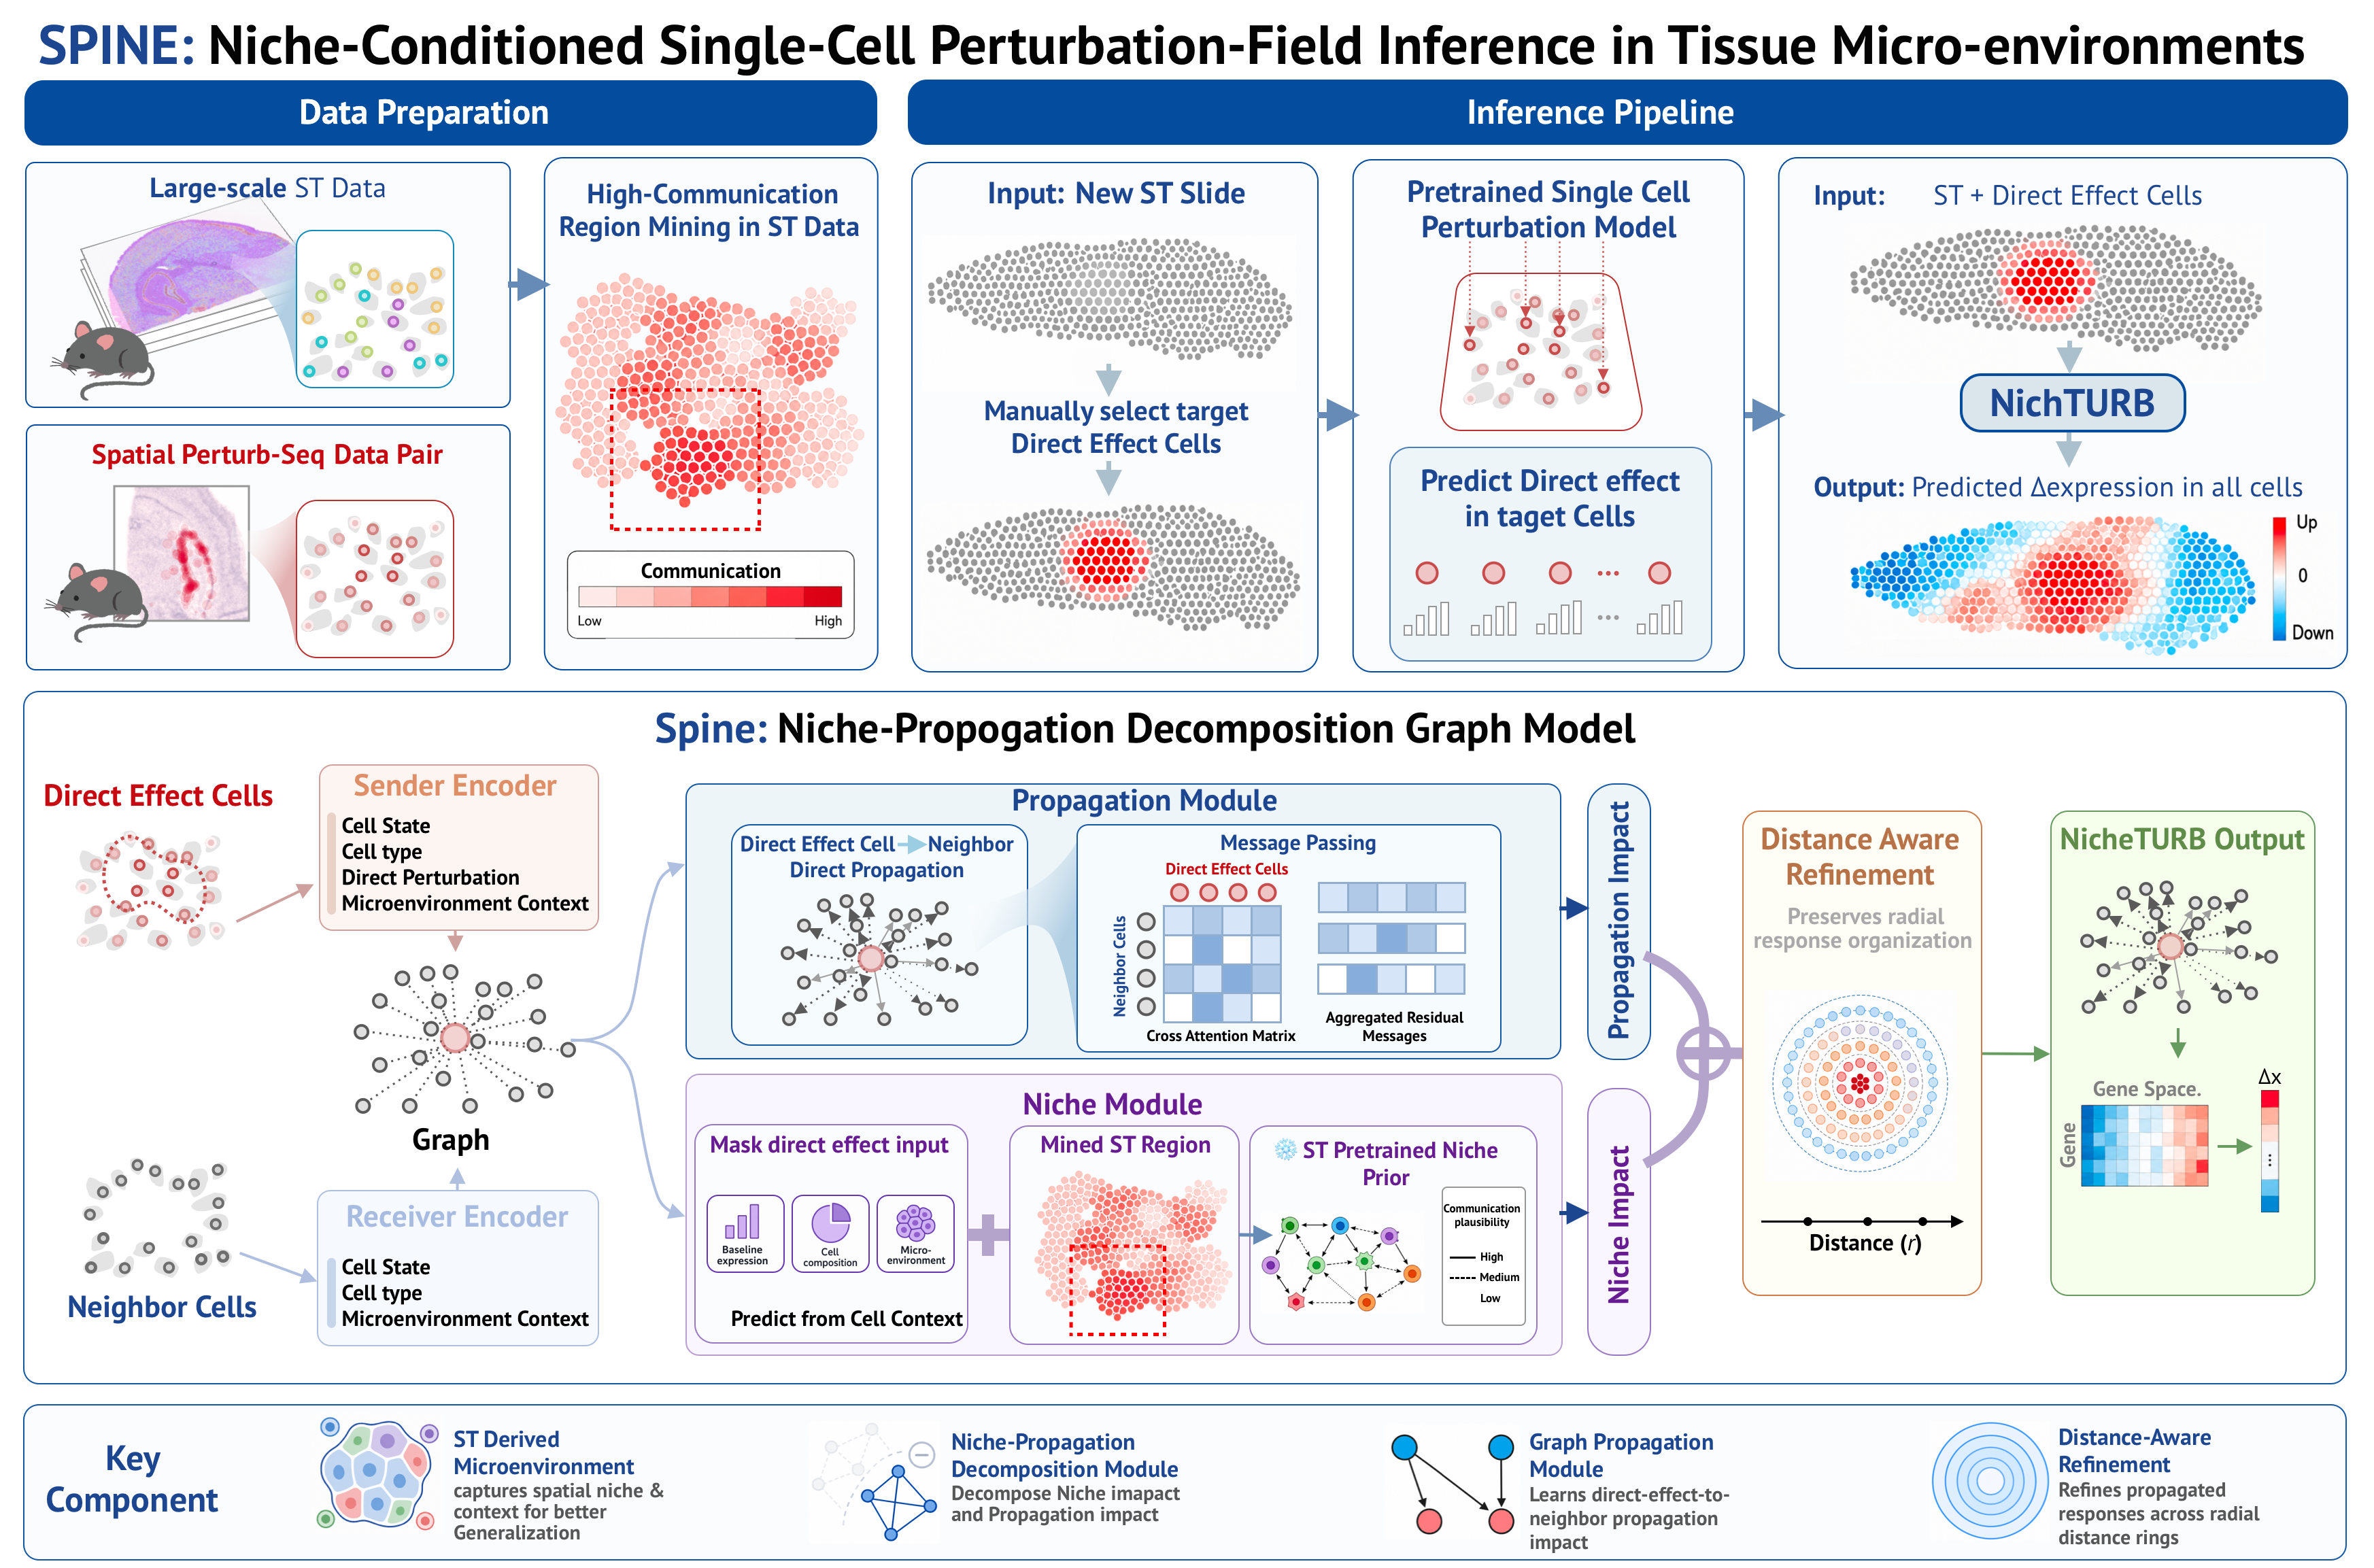
\includegraphics[width=0.98\linewidth]{model.png}
\caption{\textbf{Overview of \methodname.}
\methodname{} predicts spatial perturbation response fields from an unperturbed
cell-resolved tissue graph and a direct-effect seed. The core model first
estimates context-explainable response and then routes a direct-effect profile
from sender cells to receivers. Their sum is a signed cell-by-gene response
delta used to reconstruct the predicted post-perturbation field. The
decomposition is predictive rather than causal; reference-ST and cached
communication priors shown in the architecture are evaluated only as optional
diagnostics.}
\label{fig:main_framework}
\end{figure*}



\section{Introduction}
Spatial functional genomics measures perturbations within intact tissue and
preserves molecular changes in situ
\citep{dhainaut2022spatialcrispr,binan2025perturbfish,shen2026spatialperturbseq}.
Unlike dissociated Perturb-seq, these assays reveal whether an intervention
remains local or reorganizes distant and off-program responses. Because sparse,
costly assays cannot cover every perturbation--context pair, predictive models
must distinguish perturbation signal from tissue context.

High neighbor-expression correlation can reflect anatomy, cell state, or local
composition instead of perturbation propagation. Spatial variance and multiview
models attribute substantial expression variation to intrinsic and
environmental components
\citep{arnol2019svca,tanevski2022misty,fischer2023ncem}. In a perturbation
assay, measured neighbor fields therefore mix context with a weaker
perturbation component, which flat cell--gene correlation can obscure.

We ask how much neighbor response is predictable from context, where
perturbation signal remains, whether it transfers across regions, guides, and
assays, and whether predicted fields can preserve local response while reducing
collateral burden.
On the fully separated spatial split, context-only and full models reach pooled
Ring Pearson 0.3626 and 0.4111, with mean graph-paired lift $+0.0532$.
Predictive $R^2$ increases from 0.3712 to 0.4669, corresponding to partial
$R^2=0.1521$ conditional on context. Matching decoupling retains positive lift
without expression overlap, but not without spatial matching. Across five
guide-held-out folds, assay-matched seeds transfer modestly, whereas external
scRNA seeds do not. A validation-frozen selector preserves target qualification
while reducing held-out burden by 12.0\%.

These results support a more specific conclusion than ``the full field is
predictable'': spatial perturbation fields are \emph{globally
context-dominated but locally perturbation-structured}.




\begin{figure*}[t]
\centering
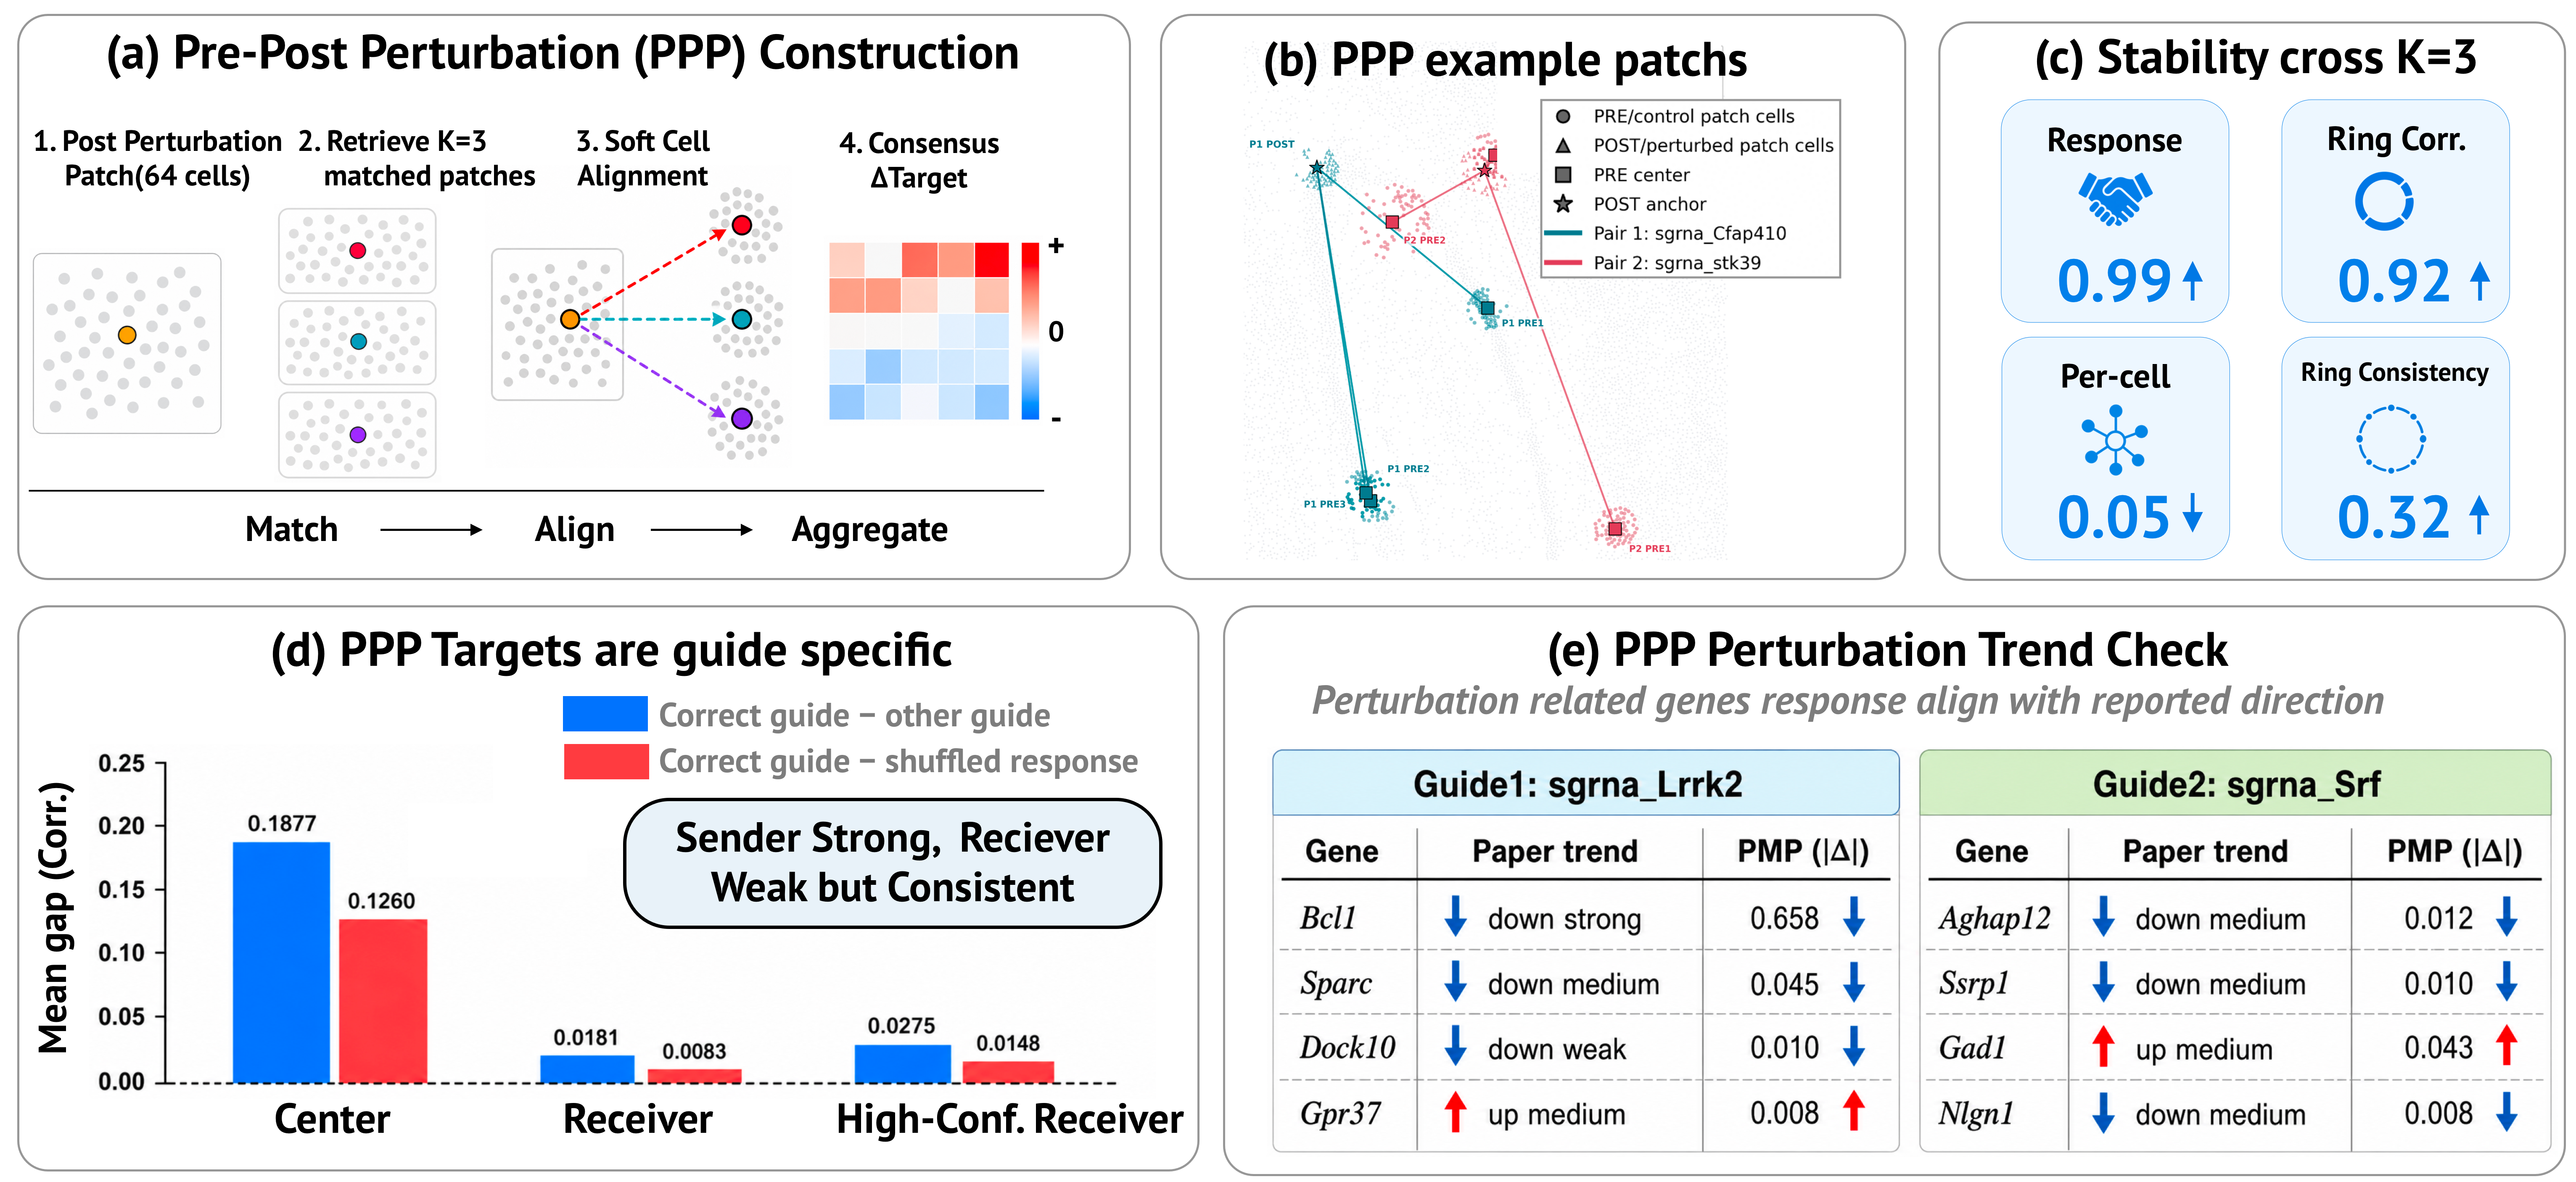
\includegraphics[width=0.9\linewidth]{pair_2.png}
\caption{\textbf{Pre-Post Perturbation Pairing (PPP) construction and validation.}
(a) Each post-perturbation 64-cell patch is matched to K=3 control patches, softly aligned, and aggregated into a consensus post--pre response target. (b) Example matched pre/post patches. (c--e) Stability and null audits show that PPP targets are consistent across matched controls and align more strongly with their own guide signatures than with wrong-guide or shuffled nulls. Consensus/ring correlations are $0.944/0.923$, and 512-gene own-guide alignment exceeds wrong-guide and target-shuffled nulls for both center cells and neighbor cells. Expression-decoupled, gene-disjoint, channel-removal, and no-spatial audits are reported in \Cref{tab:confirmatory_analysis}.}
\label{fig:data_pair}
\end{figure*}


\paragraph{Contributions.}
\begin{itemize}
    \item \textbf{An independent predictive decomposition.}
    We quantify context and perturbation signal on a fully separated spatial
    split using graph-paired lift and partial $R^2$.
    \item \textbf{An audited \ppp benchmark.}
    We separate matching and output genes, remove expression channels, and test
    profile/location controls across spatial scales.
    \item \textbf{A parsimonious response-field model and transfer analysis.}
    \methodname{} routes direct-effect profiles to receivers and distinguishes
    conditional guide transfer from failed cross-assay seed transfer.
    \item \textbf{A formal drug and perturbation selection task.}
    We evaluate target-retaining, lower-burden selection on frozen validation
    and test partitions and audit the same decision interface in external
    chemical-response assays, while treating earlier biological cases as
    exploratory.
\end{itemize}
\section{Related Work}
% \textbf{Spatial transcriptomics and spatial functional genomics.}
% Spatial transcriptomics enables gene-expression profiling with tissue coordinates, and recent high-resolution platforms and atlas-informed mapping methods improve cell-state interpretation in situ \citep{Stahl2016,Rodriques2019,Rao2021,Kleshchevnikov2022}. Spatial functional genomics further couples perturbations with intact-tissue readouts, making it possible to observe local and distal perturbation effects within native microenvironments \citep{Shen2026}. \methodname{} addresses the complementary prediction problem: given measured or predicted direct effects in sender cells, it predicts how responses propagate to spatial receivers.
\textbf{Context in spatial molecular data.}
SVCA decomposes spatial molecular variation into intrinsic, environmental, and
cell--cell interaction components~\citep{arnol2019svca}; MISTy models
intraview, juxtaview, and paraview effects~\citep{tanevski2022misty}; and NCEM
predicts expression from a spatial graph and niche composition
\citep{fischer2023ncem}. These methods motivate our context audit, but do not
condition a cell-resolved perturbation-response field on a direct-effect
profile.
\textbf{Single-cell perturbation modeling.}
Dissociated perturbation assays provide the main supervision for cell-intrinsic
response prediction, including Perturb-seq and CROP-seq
\citep{dixit2016perturbseq,adamson2016crispr,datlinger2017cropsseq}, combinatorial
and direct-capture Perturb-seq
\citep{norman2019combinatorial,replogle2020directcapture,replogle2022mapping},
Perturb-CITE-seq~\citep{frangieh2021multimodal}, and chemical-perturbation
benchmarks such as sci-Plex and OP3~\citep{srivatsan2020massively,szalata2024op3}.
Models built on these resources include conditional generative methods
\citep{lotfollahi2019scgen,lotfollahi2020trvae,Lotfollahi2023,hetzel2022chemcpa,kana2023scvidr,yu2025perturbnet},
optimal-transport and graph-based methods \citep{bunne2023cellot,roohani2023gears},
disentangled representation learning~\citep{piran2024biolord}, and foundation
models \citep{theodoris2023geneformer,cui2024scgpt,hao2024scfoundation}. These
methods provide useful direct-effect priors, but they operate on dissociated cells
and do not model direct-effect-to-neighbor propagation through local tissue graphs.
\textbf{Spatial functional genomics and response prediction.}
Perturb-map~\citep{dhainaut2022spatialcrispr},
Perturb-FISH~\citep{binan2025perturbfish}, and Spatial
Perturb-seq~\citep{shen2026spatialperturbseq} place interventions within intact
tissue. These assays reveal context-shaped effects but remain sparse across
perturbations and niches.
Recent tissue-level methods begin to connect perturbations with spatial context.
SpatialProp~\citep{spatialprop2025} propagates perturbation effects over spatial
graphs, Celcomen~\citep{celcomen2026} separates intra- and intercellular regulation
with causal generative modeling, and CONCERT~\citep{concert2025} predicts
niche-aware spot-level responses. \methodname{} targets a narrower interface:
given a sender region and measured or predicted direct-effect profile, estimate
a signed receiver field and quantify lift over context and seed nulls.








\section{Problem and Benchmark}
\label{sec:data_construction}
\subsection{Pre--Post Perturbation Pairing (PPP) Construction}
For each guide-positive anchor $a$, we form a 64-cell post-perturbation patch
$P(a)=\{a\}\cup\mathcal{N}_{63}(a)$. Because the same cells are not observed
before and after perturbation, \ppp constructs a pseudo-pre-state by matching
the complete post patch to non-perturbed or control-like patches. Candidate
controls are ranked by spatial proximity, center-expression similarity,
patch-expression similarity, and nominal cell-type composition; the top
$K=3$ matches are softly aligned and aggregated into a consensus
post-minus-matched-pre response target.

\textbf{Target provenance and audit.}
Spatial partitions are assigned before matching, so no held-out post anchor or
matched-control patch enters training. Consensus and Ring consistency are
0.944 and 0.923. Across 512 genes, own-guide versus wrong-guide alignment is
0.317 versus 0.129 at the center, 0.022 versus 0.004 in high-confidence
receivers, and 0.029 versus 0.001 over all receivers. Because matching and
model inputs partly overlap, \ppp is treated as a stable, guide-consistent
pseudo-target rather than a causal counterfactual. Expression-decoupled and
channel-removal audits are reported in \Cref{tab:confirmatory_analysis}.




\subsection{Evaluation Splits and Scope}
\label{sec:st_microenvironment_mining}
We use two evaluation regimes. The original exact-task comparison uses all
development graphs and 928 block-held-out test graphs so that the implemented
alternatives can be compared on the same output. The strict confirmatory split
uses 1,342 training, 837 validation, and 928 test graphs from fully separated
spatial regions. All perturbation-specific effect sizes, matching audits,
spatial-scale analyses, and formal selector estimates use this strict split.
Pooled Ring Pearson concatenates Ring summaries across graphs. Graph-paired
Ring lift first computes full-minus-context change within each graph and then
averages, so it is not the difference of pooled correlations. Predictive
partial $R^2$ is
$1-\mathrm{SSE}_{\mathrm{full}}/\mathrm{SSE}_{\mathrm{context}}$.

We also evaluated an unperturbed reference-ST adapter trained on two HD and
three Xenium mouse-brain studies. Its paired Ring gains are $+0.0009$,
$+0.0002$, and $+0.0032$ at 10\%, 25\%, and 50\% paired-data fractions, with
approximately $+0.0005$ at full data. We therefore exclude it from the core
\methodname{} definition and retain it only as a negative appendix diagnostic.
\section{Method}
\label{sec:method}

\subsection{Task and Predictive Decomposition}
\label{sec:method_overview}

\noindent\textbf{Task and graph interface.}
Given a cell-resolved ST slide, a perturbation query, and a sender region,
\methodname{} predicts a signed response $\widehat\Delta_i$ for every cell in a
local directed graph $P=(V,E)$. Each cell has matched-control expression
$x_i\in\mathbb{R}^G$, nominal state $c_i$, relative coordinate $p_i$, local
geometry $g_i$, direct-effect indicator $a_i$, and direct-effect profile $d_i$
when $a_i=1$; receiver cells have $a_i=0$ and $d_i=0$. Edge features $e_{ij}$
encode relative geometry, nominal state pairs, and an optional communication
compatibility score.

\noindent\textbf{Predictive decomposition.}\par\noindent
\methodname{} separates context prediction from a perturbation residual:
\begin{equation}
\label{eq:niche_prop_decomposition}
\begin{aligned}
\widehat\Delta_i
&= \widehat C_i + \widehat R_i,\\
\widehat x_i^{\mathrm{post}}
&= x_i+\widehat\Delta_i .
\end{aligned}
\end{equation}
Here $\widehat C_i$ is the response predictable from local tissue context and
$\widehat R_i$ is the remaining perturbation-conditioned response. This is a
predictive decomposition. It does not identify a causal communication pathway
or imply that every residual response was transmitted from direct-effect cells.

\subsection{Context-Explainable Component}
\label{sec:method_niche_impact}

The context model is trained with perturbation inputs masked:
\begin{equation}
\label{eq:niche_module_target}
\begin{aligned}
\widehat C_i
&= f_{\mathrm{context}}(x,c,p,e;\,a=0,d=0),\\
R_i^\star
&= \Delta_i^{\mathrm{PPP}}-\widehat C_i .
\end{aligned}
\end{equation}
It is trained first and frozen before residual-model optimization. The residual
target $R_i^\star$ asks the second stage to model response remaining after the
implemented context predictor rather than the complete context-dominated field.

\subsection{Direct-Effect-Conditioned Residual Routing}
\label{sec:method_graph_propagation}

\noindent\textbf{State initialization.}
Each cell is embedded from matched-control and spatial features, then split into a neighbor state and a direct-effect state:
\begin{equation}
\label{eq:state_initialization}
\begin{aligned}
h_i
&= \phi_x(x_i)+\phi_c(c_i)+\phi_p(p_i)+\phi_g(g_i),\\
b_i
&= \phi_N(h_i),\qquad n_i^0=0,\\
u_i
&= a_i\phi_D([h_i,d_i,g_i]) .
\end{aligned}
\end{equation}
The direct-effect state $u_i$ is nonzero only for direct-effect cells.
Receivers therefore never directly observe the perturbation profile $d_i$.

\noindent\textbf{Directed message passing.}
For direct-effect cell $i$ and neighbor cell $j$, the propagation module computes gated messages along graph edges and updates neighbor states:
\begin{equation}
\label{eq:directed_message_passing}
\begin{aligned}
z_{ij}^{\ell}
&= \sigma\!\left(\phi_a([u_i,b_j,n_j^\ell,e_{ij}])
   +w_{\mathrm{comm}}q_{ij}\right),\\
\mu_{ij}^{\ell}
&= z_{ij}^{\ell}\phi_\mu([u_i,b_j,e_{ij}]),\\
n_j^{\ell+1}
&= \operatorname{LN}\!\left(n_j^\ell+
   \sum_{\substack{i:(i,j)\in E\\ a_i=1}}\mu_{ij}^{\ell}
   \right)+\phi_u([n_j^\ell,b_j]).
\end{aligned}
\end{equation}
Direct-effect states remain fixed, and the implementation retains only edges
whose source is a direct-effect cell and destination is a receiver. There is no
receiver-to-receiver message path in the core model. Communication scores are
optional gate biases. Randomizing cached scores leaves Ring Pearson unchanged
(0.4574 versus 0.4575), so we do not attribute the perturbation-specific lift
to this prior. The base residual is decoded as
\begin{equation}
\label{eq:base_propagation_impact}
\begin{aligned}
\widehat R_i^{\mathrm{base}}
&= a_i\psi_{\mathrm{direct}}(u_i)
 +(1-a_i)\psi_{\mathrm{receiver}}([b_i,n_i^L]).
\end{aligned}
\end{equation}


\subsection{Optional Distance-Aware Refinement}
\label{sec:method_st_refinement}

After the first propagation pass, high-response neighbor cells are grouped into three distance rings around the direct-effect region: the nearest eight neighbors, the next 24 neighbors, and the remaining neighbors. Ring tokens summarize first-pass response structure and are injected into a second lightweight propagation pass, producing an ST-conditioned propagation impact $\widehat I_i^{\mathrm{prop},\mathrm{st}}$. The refinement is restricted to direct-effect cells and selected high-response neighbors, so it corrects spatially organized response patterns rather than uniformly rewriting the full patch. The final response is
\begin{equation}
\label{eq:final_response_prediction}
\begin{aligned}
\widehat\Delta_i
&= \widehat C_i
 + (1-\alpha)\widehat R_i^{\mathrm{base}}\\
&\quad + \alpha\widehat R_i^{\mathrm{refine}},
\qquad \alpha=0.65 .
\end{aligned}
\end{equation}
All terms are response deltas. We report this module as optional refinement,
not as the source of the core perturbation-conditioned effect.

\subsection{Training and inference}
\label{sec:training_inference}

The residual model is optimized with the implemented objective:
\begin{equation}
\label{eq:training_objectives}
\begin{aligned}
\mathcal{L}_{\mathrm{prop}}
&= \mathcal{L}_{\mathrm{neighbor}}
 + 0.3\mathcal{L}_{\mathrm{ring}}\\
&\quad
 + 0.3\mathcal{L}_{\mathrm{post}}
 + 0.1\mathcal{L}_{\mathrm{rank}} .
\end{aligned}
\end{equation}
Here $\mathcal{L}_{\mathrm{neighbor}}$ is Huber loss over high-confidence
receivers, $\mathcal{L}_{\mathrm{ring}}$ supervises three Ring summaries,
$\mathcal{L}_{\mathrm{post}}$ reconstructs post-state expression, and
$\mathcal{L}_{\mathrm{rank}}$ preserves within-graph gene-response ordering.
Direct-effect-cell loss has weight zero in the reported propagation setting so
the easier sender task does not dominate receiver learning. At inference,
$d_i$ is measured in the spatial assay or supplied by an external
direct-effect assay, then routed through the frozen graph model. Full
implementation details are provided in \Cref{app:method_full_details}.

\subsection{Spatially Constrained Perturbation Prioritization}
\label{sec:intervention_method}
For action $a$, target program $t$, and requested Ring $r$, utility
$U(a;t,r)$ is the signed target-program response. Collateral burden combines
far-field, off-program, and validation-defined undesirable-program response:
\begin{equation}
S(a;t,r)=\lambda_{\mathrm{far}}S_{\mathrm{far}}
+\lambda_{\mathrm{off}}S_{\mathrm{off}}
+\lambda_{\mathrm{undes}}S_{\mathrm{undes}}.
\label{eq:burden}
\end{equation}
The constrained selector is
\begin{equation}
a^\star=\arg\min_{a:\widehat U(a)\geq\tau}\widehat S(a).
\label{eq:selector}
\end{equation}
Program definitions, weights, threshold $\tau$, and the operating point are
selected on validation data and then frozen. Observed test fields are used only
for evaluation. This formal analysis is separate from exploratory post-hoc
case discovery.

The action variable is generic: it may denote a guide--site pair, a
drug--dose--time intervention, or another perturbation applied in a specified
context. Equation~\ref{eq:selector} therefore defines a response-field-based
drug and perturbation selector whenever the corresponding action-level fields
are available. When $S_{\mathrm{undes}}$ is constructed from prespecified
stress, apoptosis, or other undesirable programs, we describe it as a
toxicity-associated transcriptomic burden. It is an experimental-prioritization
proxy rather than a measurement of organismal or clinical toxicity.

The confirmatory pipeline separates target qualification from burden ranking.
Predicted utility first defines the eligible action set; a burden head then
ranks only eligible actions, and the lowest predicted-burden candidate is
selected. Candidate burden scores and the number of retained candidates are
compared on the validation region only. The frozen test analysis uses 36 target
specifications and reports target-qualified rate (TQR), observed burden
reduction relative to target-only selection, absolute burden change, pairwise
burden-order agreement, and coverage. This constrained evaluation prevents a
method from appearing successful merely by selecting weak interventions with
small responses everywhere.

\begin{figure*}[t]
\centering
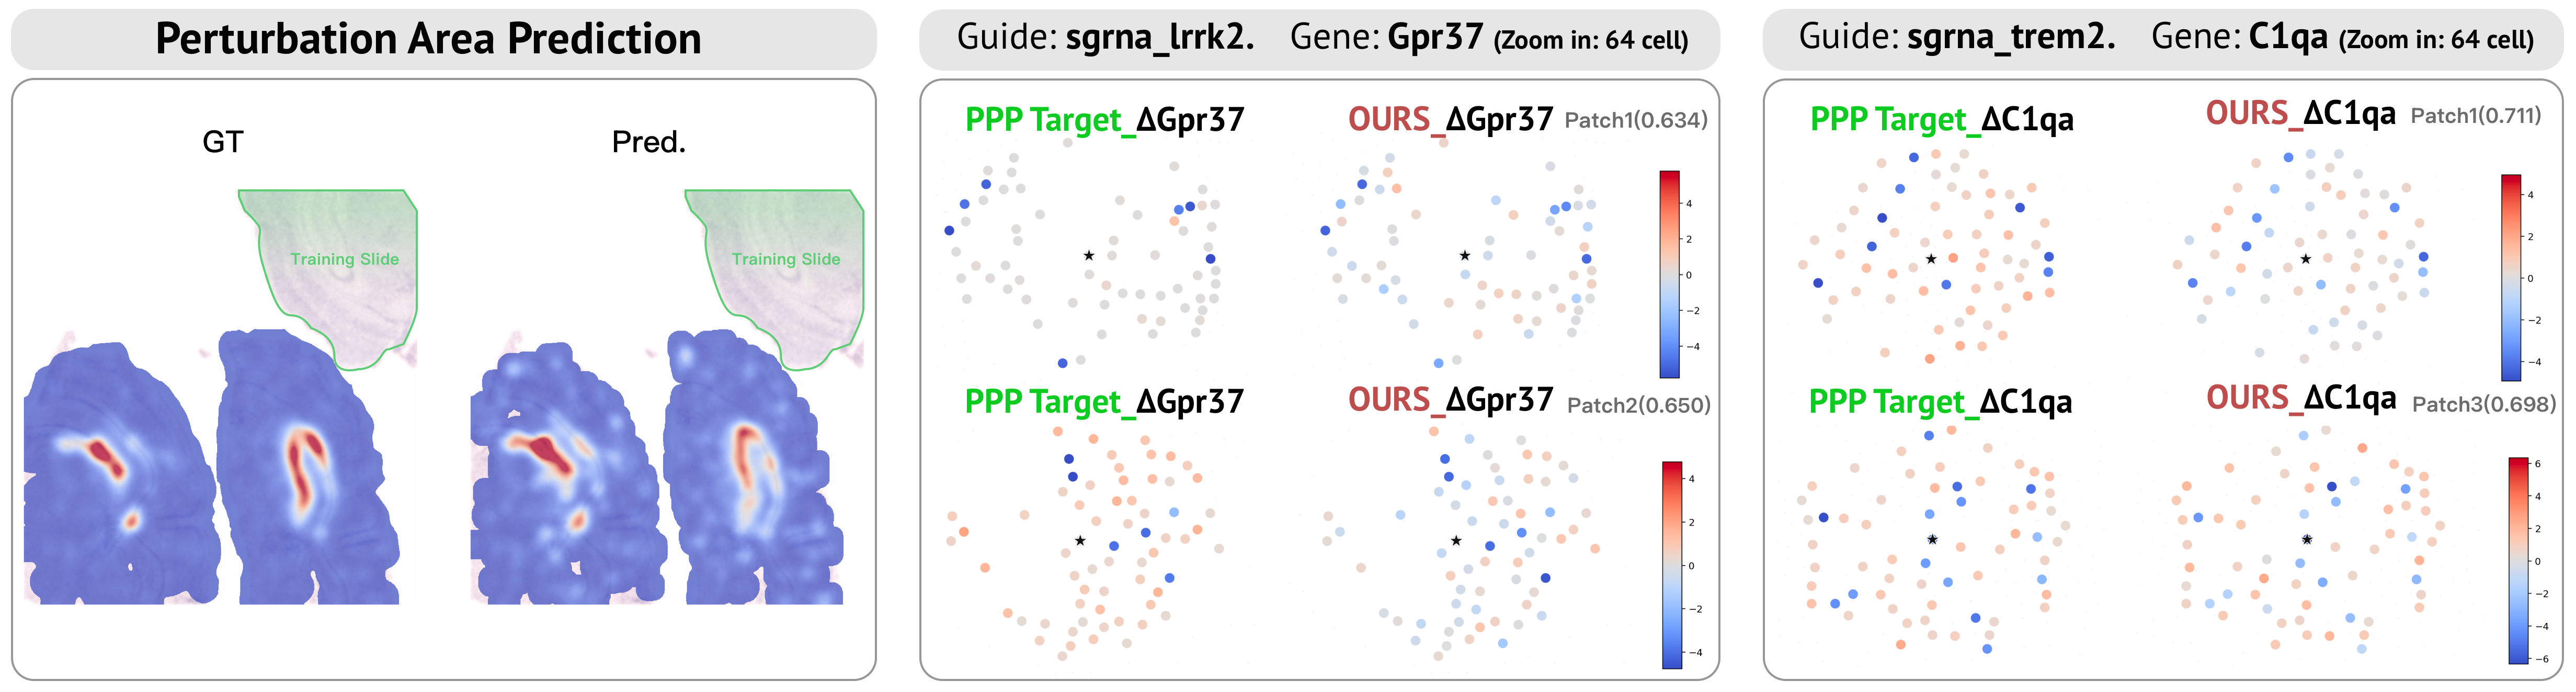
\includegraphics[width=0.90\linewidth]{main_exp.png}
\caption{\textbf{Qualitative response-field predictions on the held-out Spatial
Perturb-seq test region.}
The left panel compares the whole-region PPP pseudo-target and \methodname{}
prediction. The remaining panels show representative 64-cell neighborhoods
for \textit{Gpr37} under sgRNA-\textit{Lrrk2} and \textit{C1qa} under
sgRNA-\textit{Trem2}. Colors denote signed response deltas and stars mark
direct-effect cells. Quantitative conclusions use all 928 test graphs and all
512 genes.}
\label{fig:main_exp}
\end{figure*}

\begin{table*}[t]
\centering
\caption{\textbf{Validation across exact, controlled synthetic, and Spot level spatial perturbation datasets.}
(a) Gene-centric neighbor-cell performance on the exact cell-resolved Spatial Perturb-Seq benchmark.
(b) Controlled synthetic LR-propagation validation using external in vivo Perturb-seq direct-effect signatures.
(c) Spot/lesion-level external validation on Perturb-map.}
\label{tab:main_results}
\vspace{2pt}
\begin{minipage}[t]{0.6\linewidth}
\centering
\scriptsize
\setlength{\tabcolsep}{3.0pt}
\renewcommand{\arraystretch}{0.8}
\textbf{(a) Exact cell-resolved Spatial Perturb-Seq benchmark}
\vspace{2pt}
\resizebox{0.96\linewidth}{!}{%
\begin{tabular}{@{}lcccc@{}}
\toprule
\textbf{Gene} &
\textbf{Mean $|\Delta|$} &
\textbf{Pearson} &
\textbf{$R^2$} &
\textbf{MAE} \\
\midrule
\rowcolor{gray!18}
\multicolumn{5}{@{}l}{\textbf{\textit{Perturbation-related genes.}}} \\
\textit{Gfap}   & \pmv{0.966}{0.016} & \pmv{0.788}{0.005} & \pmv{0.621}{0.007} & \pmv{0.785}{0.008} \\
\textit{Trem2}  & \pmv{0.324}{0.006} & \pmv{0.266}{0.005} & \pmv{0.047}{0.004} & \pmv{0.449}{0.005} \\
\textit{C1qa}   & \pmv{0.996}{0.012} & \pmv{0.835}{0.003} & \pmv{0.694}{0.005} & \pmv{0.690}{0.005} \\
\textit{Olig2}  & \pmv{0.287}{0.007} & \pmv{0.184}{0.006} & \pmv{0.018}{0.004} & \pmv{0.385}{0.005} \\
\textit{Opalin} & \pmv{0.868}{0.014} & \pmv{0.781}{0.003} & \pmv{0.601}{0.006} & \pmv{0.722}{0.006} \\
\midrule
\rowcolor{gray!18}
\multicolumn{5}{@{}l}{\textbf{\textit{Top five high-variance genes.}}} \\
\textit{Ptgds}  & \pmv{1.984}{0.010} & \pmv{0.805}{0.004} & \pmv{0.645}{0.007} & \pmv{1.087}{0.011} \\
\textit{Plp1}   & \pmv{1.743}{0.014} & \pmv{0.737}{0.005} & \pmv{0.533}{0.009} & \pmv{1.174}{0.013} \\
\textit{Ywhaz}  & \pmv{2.020}{0.010} & \pmv{0.772}{0.005} & \pmv{0.540}{0.011} & \pmv{1.274}{0.017} \\
\textit{Uqcrh}  & \pmv{1.971}{0.010} & \pmv{0.790}{0.004} & \pmv{0.616}{0.008} & \pmv{1.123}{0.012} \\
\textit{Sst}    & \pmv{2.031}{0.014} & \pmv{0.773}{0.006} & \pmv{0.580}{0.011} & \pmv{1.245}{0.019} \\
\midrule
\rowcolor{gray!18}
\multicolumn{5}{@{}l}{\textbf{\textit{High-change genes.}}} \\
\textit{Cycs}   & \pmv{2.356}{0.015} & \pmv{0.851}{0.003} & \pmv{0.708}{0.007} & \pmv{1.161}{0.014} \\
\textit{Nme2}   & \pmv{2.347}{0.014} & \pmv{0.874}{0.002} & \pmv{0.762}{0.004} & \pmv{1.051}{0.010} \\
\textit{Rack1}  & \pmv{2.333}{0.011} & \pmv{0.880}{0.002} & \pmv{0.759}{0.005} & \pmv{1.056}{0.011} \\
\textit{Ptma}   & \pmv{2.203}{0.012} & \pmv{0.882}{0.002} & \pmv{0.769}{0.004} & \pmv{1.008}{0.010} \\
\textit{Psmb4}  & \pmv{2.197}{0.008} & \pmv{0.826}{0.004} & \pmv{0.673}{0.007} & \pmv{1.132}{0.013} \\
\bottomrule
\end{tabular}
}
\end{minipage}
\hfill
\begin{minipage}[t]{0.38\linewidth}
\centering
\footnotesize
\setlength{\tabcolsep}{3.0pt}
\renewcommand{\arraystretch}{0.95}
\textbf{(b) synthetic LR-propagation validation}
\vspace{2pt}
\resizebox{\linewidth}{!}{%
\begin{tabular}{@{}lccc@{}}
\toprule
\textbf{Setting} &
\textbf{Recv. $r$} &
\textbf{Ring $r$} &
\textbf{$\Delta$Ring} \\
\midrule
Niche module only & 0.003 & 0.006 & -- \\
Synthetic fine-tuned & \textbf{0.619} & \textbf{0.815} & \textbf{0.809} \\
\midrule
Held-out perturbation & 0.274 & 0.550 & 0.541 \\
Held-out interface & 0.607 & 0.806 & 0.798 \\
Held-out strength $2.0$ & 0.520 & 0.807 & 0.798 \\
Held-out host patch & 0.597 & 0.806 & 0.801 \\
\bottomrule
\end{tabular}
}
\vspace{7pt}
\textbf{(c) Spot-level Perturb-map validation}
\vspace{2pt}
\resizebox{\linewidth}{!}{%
\begin{tabular}{@{}lccc@{}}
\toprule
\textbf{Readout} &
\textbf{Spot $r$} &
\textbf{95\% CI} &
\textbf{Lesion $\rho$} \\
\midrule
\textit{Ifngr2} top-25 & \textbf{0.853} & [0.811, 0.887] & 0.536 \\
\textit{Jak2} top-25   & \textbf{0.757} & [0.702, 0.801] & \textbf{0.929} \\
\textit{Tgfbr2} top-25 & \textbf{0.714} & [0.665, 0.755] & 0.607 \\
TGF$\beta$--stroma     & \textbf{0.808} & [0.765, 0.842] & 0.750 \\
IFN response            & 0.628 & -- & -- \\
\bottomrule
\end{tabular}
}
\vspace{3pt}
\parbox{\linewidth}{\scriptsize
Panel (b) reports receiver- and ring-level correlations for controlled LR-propagation tests, including held-out perturbation, interface, strength, and host-patch settings. Panel (c) reports spot-level Pearson and lesion-level Spearman agreement after aggregating predicted response fields to Perturb-map spots.}
\end{minipage}
\vspace{-2pt}
\end{table*}




\section{Experiments}
\label{sec:experiments}
Experiments proceed from setup to response-field prediction, benchmark
evaluation, ablation and robustness analysis, and two scientific use cases.

\subsection{Experimental Setup Separates Benchmarking from Confirmatory Effects}
\label{sec:benchmark_metrics}
Mouse-brain Spatial Perturb-seq is the primary benchmark. Exact-task comparisons
use the development split; perturbation estimates use disjoint
train/validation/test graph sets (1,342/837/928). Five grouped guide-out folds
test every guide once. The spatial partitions are non-overlapping tissue blocks;
no anchor, matched control, or pseudo-target crosses them. Spatial seeds test
conditional propagation; scRNA seeds test the end-to-end interface. Unless
noted, runs use 64-cell patches on one RTX A6000.

Neighbor Pearson measures the signed receiver field, centered Pearson removes
graph offsets, Ring Pearson tests radial organization, and Neighbor MAE measures
absolute error. Mechanistic analyses compare context and full predictions per
graph; uncertainty resamples blocks or guides. Cells within a graph are never
treated as independent biological replicates.






\begin{table*}[t]
\centering
\begin{minipage}[t]{0.49\linewidth}
\centering
\caption{Main benchmark against exact-task alternative models.}
\label{tab:main_baseline_comparison}
\scriptsize
\setlength{\tabcolsep}{2.5pt}
\renewcommand{\arraystretch}{1.00}
\resizebox{\linewidth}{!}{%
\begin{tabular}{lcccc}
\toprule
Baseline & Neighbor $\uparrow$ & Centered $\uparrow$ & Ring $\uparrow$ & MAE $\downarrow$ \\
\midrule
\rowcolor{gray!18}
\multicolumn{5}{l}{\textbf{\textit{Trivial, statistical, and retrieval baselines.}}} \\
Zero-delta & 0.000 & 0.000 & 0.000 & 0.453 \\
Guide$\times$type$\times$ring mean & 0.007 & -0.000 & 0.017 & 0.468 \\
Nearest patch transfer & 0.000 & -0.001 & 0.010 & 0.612 \\
\midrule
\rowcolor{gray!18}
\multicolumn{5}{l}{\textbf{\textit{Direct-effect and radial alternatives.}}} \\
Direct-effect diffusion & 0.006 & 0.000 & 0.014 & 0.459 \\
CCC-gated linear & -0.002 & 0.003 & 0.001 & 0.510 \\
Direct-effect broadcast & 0.016 & -0.000 & 0.053 & 0.835 \\
Direct-effect broadcast, fixed decay & 0.015 & 0.003 & 0.053 & 0.594 \\
Learned radial ridge & 0.023 & -0.002 & 0.066 & 0.527 \\
\midrule
\rowcolor{gray!18}
\multicolumn{5}{l}{\textbf{\textit{Supervised patch and graph alternatives.}}} \\
Elastic-net regression & 0.570 & 0.594 & 0.391 & 0.427 \\
Patch MLP & 0.272 & 0.444 & 0.087 & 0.677 \\
Graph Transformer patch model & 0.543 & 0.564 & 0.393 & 0.460 \\
Neural CCC-GNN & 0.543 & 0.565 & 0.393 & 0.464 \\
\midrule
\rowcolor{gray!18}
\multicolumn{5}{l}{\textbf{\textit{Niche--propagation model.}}} \\
\rowcolor{cyan!10}
\methodname{} final & \textbf{0.684} & \textbf{0.715} & \textbf{0.457} & \textbf{0.408} \\
\bottomrule
\end{tabular}%
}
\end{minipage}
\hfill
\begin{minipage}[t]{0.49\linewidth}
\centering
\caption{Input-effect and structural diagnostics on controlled synthetic and real benchmarks.}
\label{tab:seed_shortcut_controls}
\scriptsize
\setlength{\tabcolsep}{3pt}
\renewcommand{\arraystretch}{1.03}
\resizebox{\linewidth}{!}{%
\begin{tabular}{lccc}
\toprule
Diagnostic & Neighbor $\uparrow$ & Ring $\uparrow$ & Lift \\
\midrule
\rowcolor{gray!18}
\multicolumn{4}{l}{\textbf{\textit{Controlled synthetic LR ablation.}}} \\
Niche module only & 0.003 & 0.006 & \textemdash \\
Shuffle direct effect & 0.069 & 0.089 & $+0.000$ \\
Predicted direct effect & 0.611 & 0.803 & $+0.714$ \\
\rowcolor{cyan!10}
Final, measured direct effect & \textbf{0.619} & \textbf{0.815} & \textbf{$+0.726$} \\
\midrule
\rowcolor{gray!18}
\multicolumn{4}{l}{\textbf{\textit{Spatial Perturb-Seq ablation.}}} \\
Niche module only & 0.610 & 0.405 & \textemdash \\
Shuffle direct effect & 0.679 & 0.405 & $+0.000$ \\
Predicted direct effect & 0.680 & 0.417 & $+0.012$ \\
\rowcolor{cyan!10}
Final, measured direct effect & \textbf{0.684} & \textbf{0.457} & \textbf{$+0.052$} \\
\midrule
No niche-impact residualization & 0.165 & 0.153 & \textemdash \\
No edge attributes & 0.606 & 0.418 & $+0.013$ \\
No direct-effect input & 0.614 & 0.441 & $+0.036$ \\
\bottomrule
\end{tabular}%
}
\end{minipage}
\end{table*}





Spatial Perturb-seq determines cell-resolved claims; controlled
LR propagation, Perturb-map, and Perturb-FISH test known-rule
recovery, spot/lesion transfer, and native-panel burden ranking, respectively.
Supporting assays probe distinct failure modes across assays and are not pooled;
the appendix reports full settings and resampling units.








\subsection{\methodname{} Reconstructs Cell-Resolved Spatial Response Fields}
\label{sec:validation_main_benchmark}
On the exact-task comparison split, \methodname{} reconstructs cell-resolved
response fields more accurately than the implemented statistical, retrieval,
radial, linear, patch, and generic graph alternatives. It reaches
Neighbor and Ring Pearson of 0.684 and 0.457, with Neighbor MAE 0.408
(\Cref{tab:main_baseline_comparison}).
Whole-region and local-neighborhood maps recover heterogeneous signed responses,
while gene-level accuracy is strongest for high-change and high-variance genes
and remains heterogeneous for genes linked to perturbation
(\Cref{fig:main_exp,tab:main_results}). Across all 928 test
graphs and 512 genes, representative perturbation-related genes range from
Pearson 0.835 for \textit{C1qa} and 0.788 for \textit{Gfap} to 0.266 for
\textit{Trem2} and 0.184 for \textit{Olig2}; high-change genes reach
0.826--0.882 (\Cref{tab:main_results}). The displayed sgRNA-\textit{Lrrk2}
and sgRNA-\textit{Trem2} neighborhoods illustrate the same signed local
structure without determining the quantitative result
(\Cref{fig:main_exp}). Together, these results establish exact-task
reconstruction performance; because the split was used during development,
they are not estimates of perturbation-specific effect size.

\subsection{\methodname{} Outperforms Baselines and Transfers Across Spatial Assays}

Independent assays support specific parts of the response-field interface. On
controlled ligand--receptor propagation, fine-tuning raises context-only
Neighbor/Ring correlation from 0.003/0.006 to 0.619/0.815, demonstrating
learnability when the rule is known. Perturb-map program Pearson reaches
0.853, 0.757, and 0.714 for \textit{Ifngr2}, \textit{Jak2}, and
\textit{Tgfbr2}, respectively (\Cref{tab:main_results}). These results support
controlled propagation and coarse program transfer without being pooled with
the exact mouse-brain estimates.

The lower-burden decision rule also transfers at module level. On 39 reliable
Perturb-FISH specifications, predicted-utility/predicted-burden selection
reaches TQR 0.718 and burden reduction 0.151; observed-utility/predicted-burden
selection raises the reduction to 0.207, with pairwise agreement 0.851.
The spillover head increases median burden correlation from 0.539 for
aggregation to 0.855 and reaches Safe@5 of 1.0 on the reliable subset,
confirming that target retention, rather than burden ordering, is the weaker
part of the external selector.
Observed-response audits on LINCS Phase I/II, Tahoe-100M pseudobulk, and
Sci-Plex further support context-aware drug--dose--time ranking. These assays
cover 11,039, 44,696, 1,137, and 151 actions, respectively. Context-aware
selection retains median TQR 1.0 in all four resources, versus global TQR
0.567/0.600/0.640/1.000, while reducing harmful-module burden by
0.099/0.123/0.055/0.012. They therefore validate the decision formulation once
response fields exist, not end-to-end spatial drug prediction; full results
are in \Cref{app:selector_audit}.

Accurate context reconstruction alone cannot ensure reliable response
prediction. The official CONCERT implementation reconstructs native expression
strongly, but falls below a guide-mean baseline for perturbation pseudo-deltas
in all four evaluated contrasts. For example, Perturb-map \textit{Tgfbr2}
aggregate gene Pearson is 0.585 for CONCERT versus 0.884 for guide mean, while
\textit{Ifngr2} is 0.287 versus 0.808. We therefore interpret this result as an
objective mismatch rather than a definitive method ranking: reconstruction
accuracy alone is insufficient evidence of perturbation-conditioned response.
Complete values and exact-task input controls are reported with
\Cref{tab:seed_shortcut_controls} in the appendix.

\subsection{Ablations Isolate Direct-Effect Transfer, Local Signal, and Spatial Scale}
\label{sec:ablations}
\label{sec:signal_decomposition}
Assay-matched direct-effect profiles transfer conditionally to unseen guides,
whereas companion scRNA profiles do not. Across five guide-held-out folds,
observed spatial seeds raise Ring Pearson from 0.4400 to 0.4619
($+0.0220$, positive in 5/5 folds), while external scRNA seeds reduce it to
0.4130 (below zero seed in 5/5 folds). Thus, cross-assay direct-effect transfer,
not spatial routing alone, is the current end-to-end bottleneck.

Perturbation conditioning adds a reproducible radial component beyond tissue
context. On the independent three-way split, it raises pooled Ring Pearson
from 0.3626 to 0.4111, yields graph-paired lift $+0.0532$
[0.0474, 0.0586], and increases predictive $R^2$ from 0.3712 to 0.4669
(partial $R^2=0.1521$; \Cref{tab:confirmatory_analysis}, panel A). The lift remains
positive under gene-disjoint, channel-removal, and strict no-expression PPP
variants, but vanishes without spatial matching
(\Cref{tab:confirmatory_analysis}, panel C). Thus, context explains most predictable
variation, while spatially matched perturbation conditioning contributes a
smaller radial signal that is not explained solely by matching/output overlap.
The expression-decoupled variants retain lift between $+0.0257$ and $+0.0281$;
strict no-expression matching retains $+0.0128$, whereas no-spatial matching
falls to $+0.0025$ with an interval spanning zero. This attenuation identifies
local control provenance, rather than expression overlap alone, as necessary
for an informative pseudo-target.

\begin{table}[t]
\centering
\caption{\textbf{Confirmatory perturbation signal, benchmark decoupling, and
scale sensitivity.}
Panels A, C, and D use the strict three-way spatial split. Pooled Ring
correlation and graph-paired lift are different estimands. Partial
$R^2=1-\mathrm{SSE}_{\mathrm{full}}/\mathrm{SSE}_{\mathrm{context}}$.}
\label{tab:confirmatory_analysis}
\vspace{2pt}
\footnotesize
\setlength{\tabcolsep}{1.0pt}
\renewcommand{\arraystretch}{1.03}
\textbf{A. Independent spatial split}
\vspace{1pt}
\begin{tabular*}{\columnwidth}{@{\extracolsep{\fill}}lrrrr@{}}
\toprule
Metric & Context & Full & Effect & 95\% CI \\
\midrule
Pooled Ring & 0.3626 & 0.4111 & -- & -- \\
Graph-paired lift & -- & -- & $+0.0532$ & [0.0474, 0.0586] \\
Predictive $R^2$ & 0.3712 & 0.4669 & 0.1521 & [0.1476, 0.1559] \\
\bottomrule
\end{tabular*}
\vspace{5pt}

\textbf{C. PPP decoupling}
\vspace{1pt}
\begin{tabular*}{\columnwidth}{@{\extracolsep{\fill}}lrr@{}}
\toprule
PPP construction & Paired lift & 95\% CI \\
\midrule
Gene-disjoint matching/output & $+0.0257$ & [0.0215, 0.0302] \\
No center-expression matching & $+0.0281$ & [0.0244, 0.0319] \\
No patch-expression matching & $+0.0263$ & [0.0226, 0.0300] \\
Strict no-expression matching & $+0.0128$ & [0.0088, 0.0166] \\
No spatial matching & $+0.0025$ & [$-0.0022$, 0.0066] \\
\bottomrule
\end{tabular*}
\vspace{5pt}

\textbf{D. Patch-scale sensitivity}
\vspace{1pt}
\begin{tabular*}{\columnwidth}{@{\extracolsep{\fill}}lrrr@{}}
\toprule
Patch (median radius) & Context & Full & Paired lift \\
\midrule
32 cells; 67.83\,$\mu$m & 0.2775 & 0.3142 & $+0.0430$ \\
64 cells; 98.18\,$\mu$m & 0.3626 & 0.4111 & $+0.0532$ \\
100 cells; 125.79\,$\mu$m & 0.4826 & 0.4722 & $-0.0077$ \\
128 cells; 144.60\,$\mu$m & 0.4739 & 0.4470 & $-0.0246$ \\
\bottomrule
\end{tabular*}
\end{table}
Direct-effect input controls further show that profile and region both
contribute (\Cref{tab:app_profile_controls}). Shuffling the profile at the
correct region lowers Ring Pearson from 0.4574 to 0.4056, while relocating the
correct profile lowers it to 0.4314; randomizing both yields 0.4135.
Randomizing the communication prior leaves performance unchanged (0.4575), so
the lift cannot be attributed to that prior. This omitted panel B is reported
in full in the appendix.

Finally, the perturbation-conditioned signal is local in scale. Graph-paired
lift is positive for
32- and 64-cell patches ($+0.0430$ and $+0.0532$) but negative for 100 and 128
cells ($-0.0077$ and $-0.0246$), even as context Ring Pearson rises from 0.2775 at 32
cells to 0.4739 at 128 cells (\Cref{tab:confirmatory_analysis}, panel D).
Together, the input and scale controls support a profile- and
location-dependent response field at an assay-specific local scale, motivating
the 64-cell operating point without treating it as a universal biological
radius.



\begin{figure}[t]
\centering
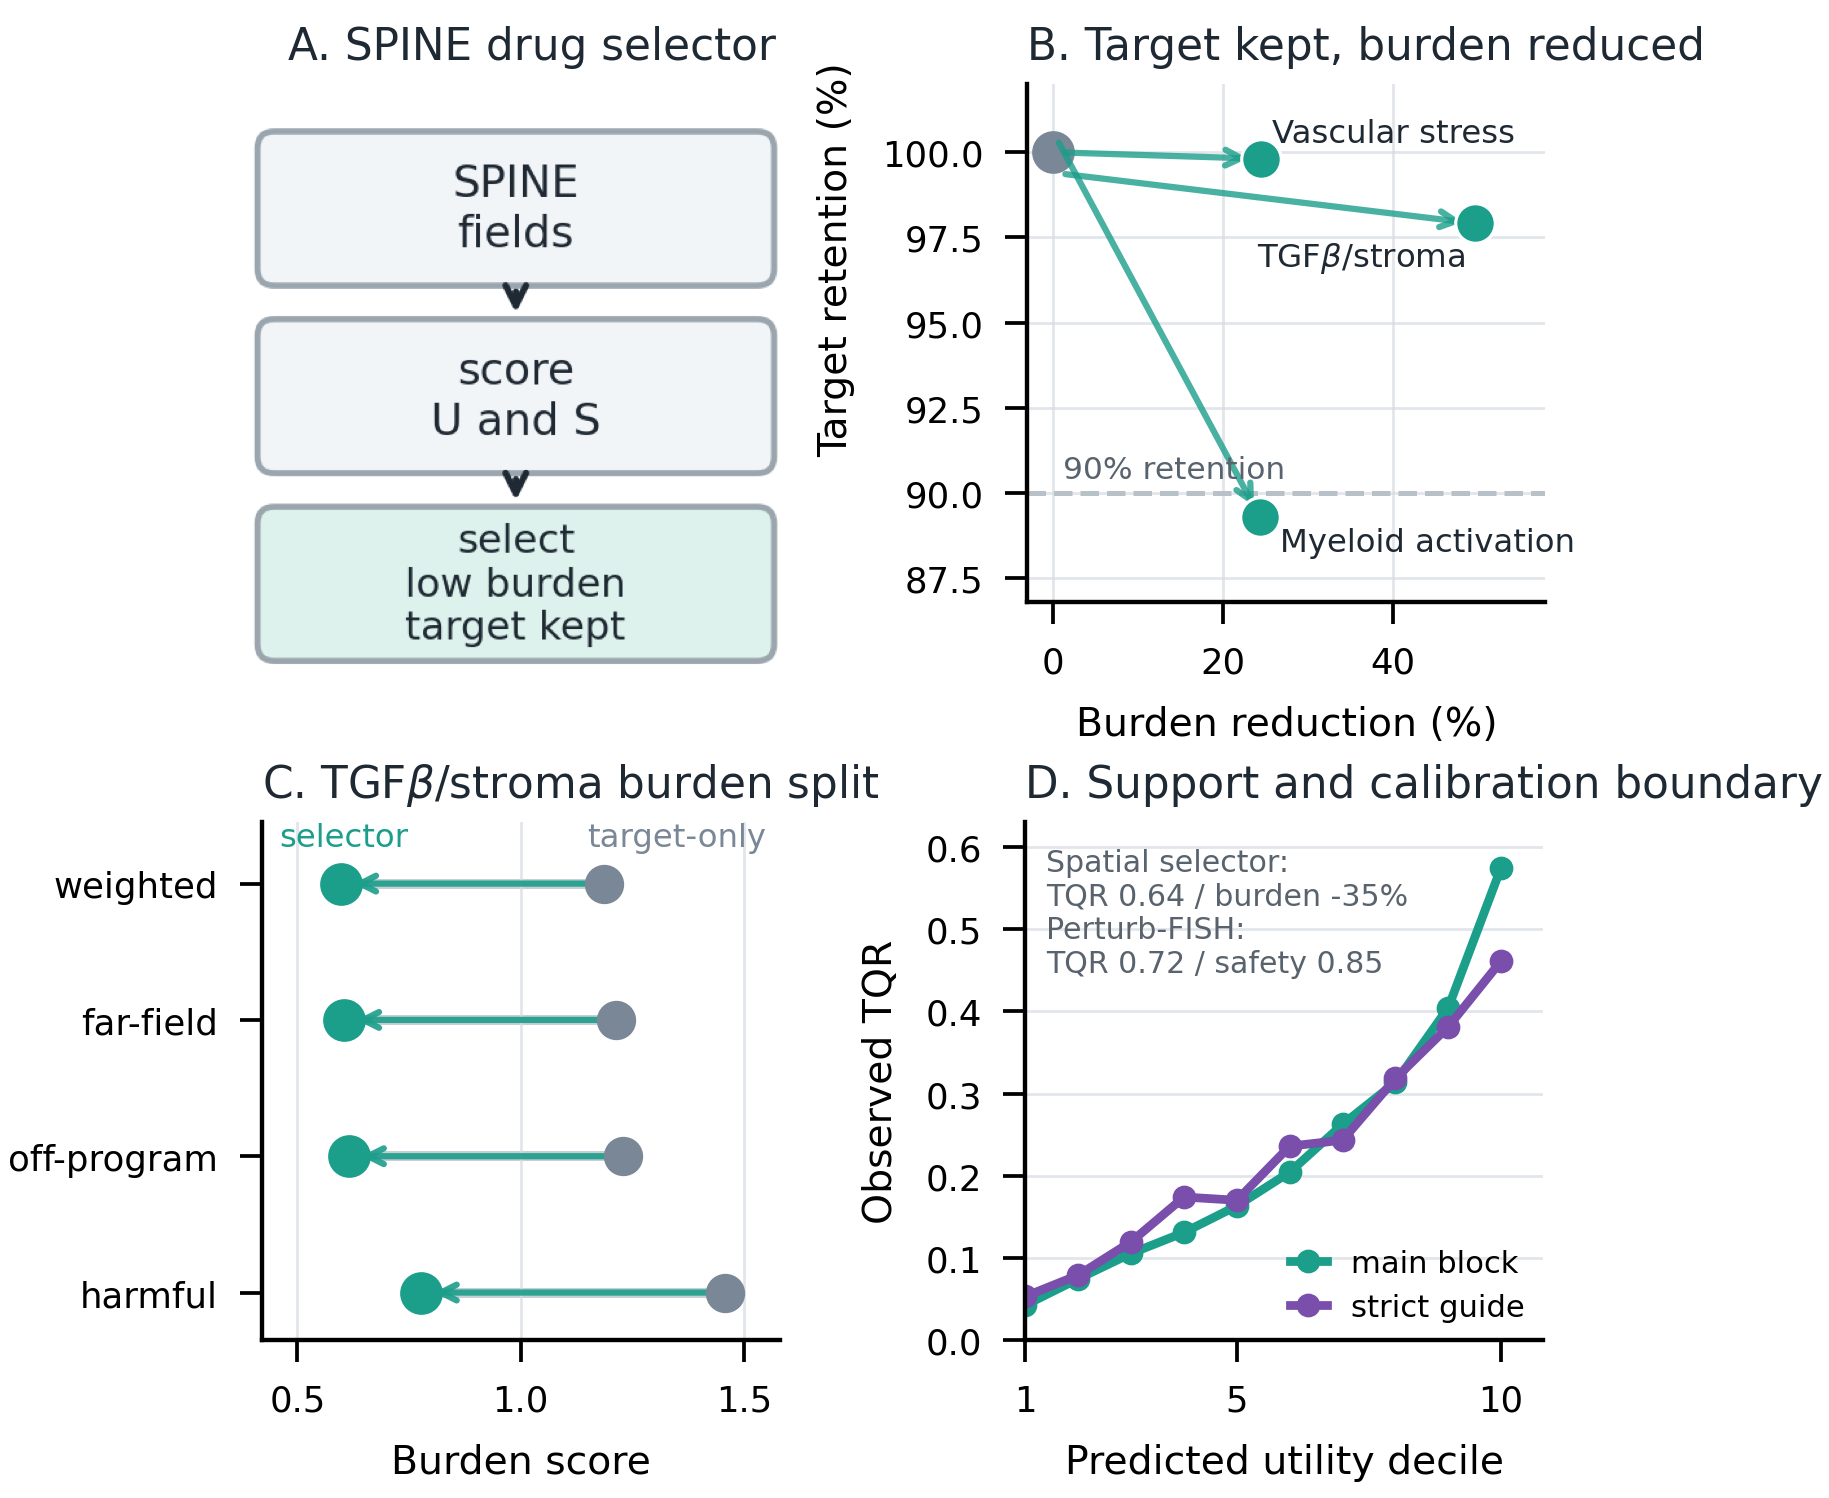
\includegraphics[width=\linewidth]{selector.png}
\caption{\textbf{Response-field-based drug and perturbation selection.}
(a) Formal field-to-decision interface. (b--c) Exploratory post-hoc cases
illustrating how matched target utility can coexist with different spatial
burden. (d) Confirmatory evaluation on the fully separated
train/validation/test selector split: the selector preserves target-qualified
rate 0.6944 while reducing mean spillover by 12.0\%; absolute held-out burden
decreases by 0.1244 [0.0559, 0.1926]. The post-hoc cases are illustrative and
are not used as confirmatory effect estimates.}
\label{fig:drug_selector_application}
\end{figure}

\subsection{\methodname{} Enables Target-Retaining, Lower-Burden Drug and Perturbation Selection}
\label{sec:drug_selector_application}
\textbf{\methodname{} turns response-field prediction into a
target-retaining, lower-burden selection problem.} Target-only ranking cannot
distinguish actions that produce comparable local utility but different
far-field or off-program responses. We therefore retain actions that satisfy a
validated local-program threshold and minimize far-field, off-program, and
undesirable-program burden. The hard utility constraint prevents an inactive
action from appearing favorable merely because all its responses are small.
When undesirable programs encode stress or apoptosis, this score is a
toxicity-associated transcriptomic burden, not organismal toxicity. All
thresholds, weights, and operating points are selected on validation data
before test evaluation.


\begin{figure}[t]
\centering
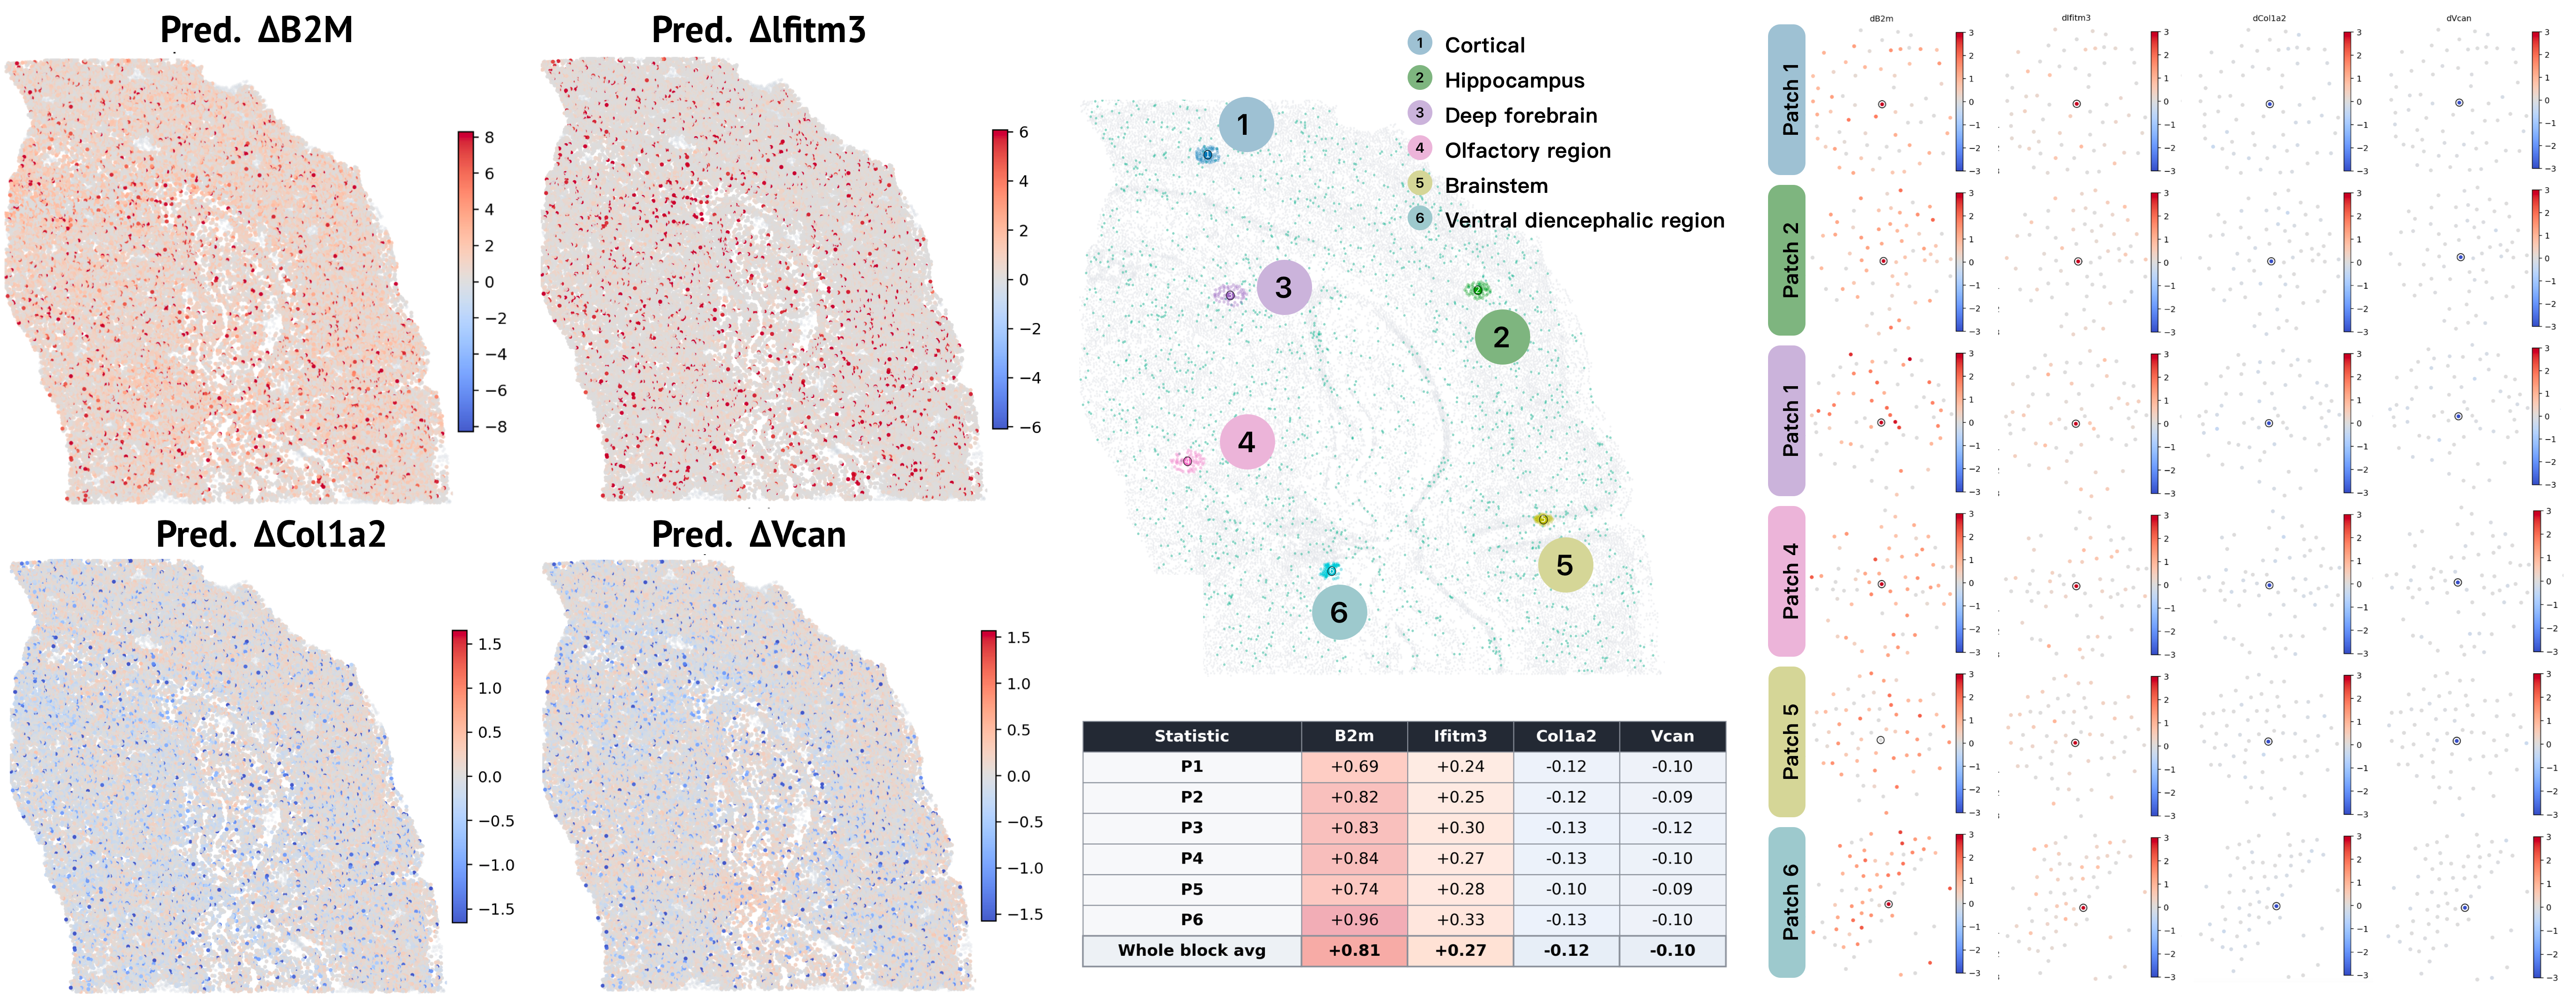
\includegraphics[width=\linewidth]{novo.png}
\caption{
\textbf{De novo IFN-$\gamma$ response-field prediction in mouse brain.}
Left: whole-tissue maps for representative IFN/MHC-I-associated and structural genes, showing positive \textit{B2m}/\textit{Ifitm3} and negative \textit{Col1a2}/\textit{Vcan} responses rather than a uniform shift.
Middle: six high-response regions with patch-averaged deltas overlaid on the spatial graph.
Right: local 64-cell neighborhoods, where highlighted target cells show the strongest response and nearby neighbors show structured propagation.}
\label{fig:ifng_response_field}
\end{figure}






\textbf{On the frozen spatial test block, the selector preserves target
qualification while lowering collateral response burden.} The test set
contains 3,107 spatially separated actions and 36 target specifications. A
five-candidate consensus fixed on validation matches the target-only
target-qualified rate (TQR; 0.6944 versus 0.6944) and reduces mean spillover by
12.0\% (\Cref{fig:drug_selector_application}). Absolute burden decreases by
0.1244 [0.0559, 0.1926], regret falls from 0.4668 to 0.3424, and Safe@5 rises
from 0.1111 to 0.4167. Random observed-qualified selection and Path2
aggregation instead yield mean reductions of $-9.8\%$ and $-16.4\%$, whereas
the dual utility/burden selector reaches $+12.9\%$
(\Cref{tab:app_selector_formal}).

\textbf{Task-specific \methodname{} burden ranking, rather than generic
aggregation, drives the improvement.} The context spillover head reaches
pairwise lower-burden agreement 0.6250 [0.6108, 0.6393], compared with 0.4909
for a context MLP. Selected actions have lower burden for 24 specifications,
higher burden for seven, and unchanged burden for five. The absolute-decrease
interval excludes zero, whereas the relative-reduction interval
[$-0.0018$, 0.2289] crosses zero because ratios are unstable when target-only
burden is small. The observed-field oracle reaches 60.6\% reduction. Thus,
burden ranking is learnable, but utility qualification and extreme-rank
calibration leave substantial headroom.

\textbf{Matched-utility cases show why spatial response fields can change which
action should be selected.} The TGF-$\beta$/stroma case retains 97.9\% of
target utility while reducing weighted burden by 49.7\%. The vascular-stress
and myeloid-activation cases retain 99.8\% and 89.3\% of target utility while
reducing burden by 24.4\% each
(\Cref{fig:drug_selector_application}). These examples expose differences in
far-field, off-program, and undesirable-program responses that target-only
ranking cannot resolve. Because the operating family and cases were explored
post hoc, they explain the decision mechanism but are not confirmatory effect
estimates.

\textbf{Observed chemical-response resources support the same constrained
interface for drug--dose--time selection.} Context-specific selection reaches
TQR 1.000 with burden reductions of 9.88\%, 12.30\%, 5.50\%, and 1.19\% in
LINCS Phase II, LINCS Phase I, the Tahoe-100M pseudobulk subset, and Sci-Plex,
respectively (\Cref{tab:app_chemical_selector}). These audits use observed
response profiles. They establish that target-retaining drug selection is a
meaningful decision problem, but do not validate end-to-end spatial drug-field
prediction, treatment efficacy, or clinical safety.
\FloatBarrier








\subsection{\methodname{}-Based IFN-\texorpdfstring{$\gamma$}{gamma} Deployment Produces a Spatially Heterogeneous Hypothesis}
\label{sec:ifng_case_study}
\textbf{\methodname{} supports de novo spatial perturbation queries when only a
non-spatial direct-effect model is available.} We apply the trained propagation
model to an intact mouse-brain spatial graph that has no paired IFN-$\gamma$
spatial perturbation labels. CPA is trained or fine-tuned on PerturbSapiens
cytokine data using treatment status (PBS/control versus IFN-$\gamma$), cell
type, and tissue or broad class as covariates. For each Sample2/pre4 spatial
cell, CPA predicts the IFN-$\gamma$ and matched control states. Their difference
defines a per-cell direct-effect delta that is passed to the \methodname{}
propagation module. This experiment demonstrates the query interface and
generates hypotheses; it is not matched spatial validation.

\textbf{The inferred field recovers a coherent canonical
IFN-$\gamma$/MHC-I response.} Target-cell deltas are positive for interferon
and antigen-presentation genes, including \textit{B2m} $(+1.91)$,
\textit{H2-D1} $(+1.57)$, and \textit{Ifitm3} $(+1.72)$
(\Cref{fig:ifng_response_field}). Their consistent direction across
high-response targets indicates that the deployment recovers a systematic
IFN/MHC-I-like program rather than an isolated marker.

\textbf{\methodname{} localizes the strongest response to immune-, vascular-,
and glial-associated niches rather than assigning a uniform tissue-wide
effect.} Microglia account for 11.91\% of top-pathway 5\% targets versus
7.98\% background frequency, corresponding to 1.49$\times$ enrichment.
Endothelial and pericyte states are also mildly enriched. This distribution is
consistent with an IFN-$\gamma$ response concentrated in immune, vascular, and
glial microenvironments rather than arbitrary spatial locations.

\textbf{The same query predicts spatially heterogeneous suppression of
structural and vascular programs.} Target cells show decreased
\textit{Col1a2} $(-1.31)$, \textit{Vcan} $(-1.28)$, and \textit{Flt1}
$(-1.82)$ alongside IFN/MHC-I activation. Whole-tissue maps and local
64-cell neighborhoods show that response direction and magnitude vary across
regions rather than forming a uniform slide-level shift
(\Cref{fig:ifng_response_field}). Seed construction and full numerical
readouts are reported in
\Cref{tab:app_ifng_direct_effect_seed,app:ifng_extended_interpretation}; direct
spatial perturbation remains necessary to validate these hypotheses.
\FloatBarrier
\section{Discussion and Conclusion}
\label{sec:discussion_conclusion}
Tissue context explains most global response-field structure, whereas
conditioning on the perturbation contributes a smaller, reproducible radial
component. This lift persists when matching and output genes are separated,
requires spatially local controls, and depends on both the direct-effect profile
and sender location.
It peaks near the 64-cell (98-$\mu$m) scale and transfers to unseen guides only
when assay-matched spatial seeds are available; external scRNA seeds
underperform zero seed. These controls support local response-field prediction
within the assayed system, not causal communication inference.

Separating absolute reconstruction from graph-paired lift is essential. Pooled
correlation rewards stable anatomical structure, whereas paired Ring lift asks
whether the correct seed reorganizes the local field beyond context. Their
disagreement is therefore diagnostic rather than contradictory and identifies
direct-effect transfer and top-action calibration as the main remaining
bottlenecks.

The validation-frozen selector shows that the remaining signal is
decision-relevant: it preserves target qualification while modestly reducing
held-out burden. The same constrained utility--burden interface also supports
drug--dose--time ranking in observed LINCS, Tahoe-100M pseudobulk, and Sci-Plex
response profiles. We therefore view \methodname{} as a response-field-based
drug/perturbation selector for experimental prioritization. The current
evidence is retrospective and the undesirable-program score is only a
toxicity-associated transcriptomic proxy, not a treatment recommendation or
clinical safety estimate. Prospective validation should select actions before
measurement, use assay-compatible direct-effect profiles, and independently
measure both target response and collateral spatial fields.

\section{Limitations and Ethical Considerations}
\label{sec:limitations_ethical_considerations}
\ppp is a matched pseudo-counterfactual, not paired pre/post measurement.
Primary effect estimates come from one mouse-brain assay, and the selected
spatial scale, program definitions, and calibration may not transfer across
tissues or platforms. Guide-OOD gains are modest, external scRNA seeds fail,
and selector results are retrospective. The chemical-response audits use
observed profiles and validate the drug-selection formulation rather than
end-to-end spatial drug-field prediction. Prospective spatial perturbation
validation is required; public data remain subject to their original consent
and use terms.

\section{Generative AI Usage}
Generative AI tools were used for language editing and code assistance during
manuscript preparation. All experimental designs, numerical results, figures,
and scientific interpretations were independently verified by the authors. No
generative AI model was used to construct benchmark targets or experimental
labels.

\section{Code and Data Availability}
\label{sec:code_release}
We will release the anonymized code, configuration files, processed split
manifests, benchmark construction scripts, and evaluation scripts in an
\href{https://anonymous.4open.science/r/NICHETURB-F5E5/}{anonymous GitHub repository}.
\clearpage
\bibliographystyle{ACM-Reference-Format}
\bibliography{references}
\clearpage
\appendix
\setcounter{table}{0}
\setcounter{figure}{0}
\renewcommand{\thetable}{S\arabic{table}}
\renewcommand{\thefigure}{S\arabic{figure}}
\renewcommand{\theHtable}{appendix.table.\arabic{table}}
\renewcommand{\theHfigure}{appendix.figure.\arabic{figure}}

\refstepcounter{section}
\makeatletter
\def\@currentlabelname{Additional Experiments and Implementation Details}
\makeatother
\label{app:additional_experiments}
\pdfbookmark[1]{Appendix: Additional Experiments and Implementation Details}{appendix-start}

\twocolumn[{
\begin{minipage}{\textwidth}
\centering
{\LARGE\bfseries Appendix\par}
\vspace{3pt}
{\large\bfseries Additional Experiments and Implementation Details\par}
\vspace{6pt}
\hrule
\vspace{6pt}

\raggedright\normalsize
\textbf{Overview.}
This appendix documents the complete evidence chain from pseudo-counterfactual
benchmark construction to response-field prediction and intervention
prioritization. Sections A.1--A.5 specify \ppp matching and transport,
communication-rich and mouse-reference microenvironment mining, task
compatibility with related resources, and the full model and training
procedure. Sections A.6--A.10 then report gene-level performance, unseen-guide
and guide-stratified stability, controlled ligand--receptor propagation, and
Perturb-map transfer. Tables S16--S21 consolidate the wide system-level,
structural, selector, and chemical-response summaries before the narrower
diagnostics.

\vspace{2pt}
Sections A.11--A.20 provide blend and reference-ST sensitivity, direct-effect
controls, development and structural ablations, the IFN-$\gamma$ deployment,
extended interpretation, the formal drug/perturbation selector audit,
whole-block visualization, and compute details. Primary quantitative claims
come from the mouse-brain Spatial Perturb-seq benchmark; synthetic,
cross-assay, and deployment analyses test distinct interfaces or failure modes
and are not pooled as equivalent evidence.

\vspace{5pt}
{\large\bfseries Appendix Contents\par}
\vspace{3pt}

\begin{minipage}{0.315\textwidth}
\raggedright\small
\textbf{Construction and model}\par
\vspace{2pt}
\hyperref[app:detailed_data_construction]{\textbf{\ref*{app:detailed_data_construction}} Detailed data construction}\par
\hyperref[app:communication_microenvironment_mining]{\textbf{\ref*{app:communication_microenvironment_mining}} Communication-rich mining}\par
\hyperref[app:mouse_microenvironment_mining]{\textbf{\ref*{app:mouse_microenvironment_mining}} Mouse reference mining}\par
\hyperref[app:resource_comparison]{\textbf{\ref*{app:resource_comparison}} Resource comparison}\par
\hyperref[app:method_full_details]{\textbf{\ref*{app:method_full_details}} Full method and training}\par
\hyperref[app:full_gene_centric_validation]{\textbf{\ref*{app:full_gene_centric_validation}} Gene-centric validation}\par
\hyperref[app:strict_guide_ood]{\textbf{\ref*{app:strict_guide_ood}} Strict guide-out stability}\par
\end{minipage}
\hfill
\begin{minipage}{0.315\textwidth}
\raggedright\small
\textbf{Robustness and transfer}\par
\vspace{2pt}
\hyperref[app:guide_stratified_stability]{\textbf{\ref*{app:guide_stratified_stability}} Guide-stratified stability}\par
\hyperref[app:synthetic_lr_validation]{\textbf{\ref*{app:synthetic_lr_validation}} Synthetic LR validation}\par
\hyperref[app:perturbmap_validation]{\textbf{\ref*{app:perturbmap_validation}} Perturb-map validation}\par
\hyperref[tab:app_full_baseline_comparison]{\textbf{Tables \ref*{tab:app_full_baseline_comparison}--\ref*{tab:app_chemical_selector}} Wide summary tables}\par
\hyperref[app:single_column_diagnostics]{\textbf{\ref*{app:single_column_diagnostics}} Single-column diagnostics}\par
\hyperref[app:blend_and_reference_diagnostics]{\textbf{\ref*{app:blend_and_reference_diagnostics}} Blend/reference diagnostics}\par
\hyperref[app:profile_controls]{\textbf{\ref*{app:profile_controls}} Direct-effect controls}\par
\end{minipage}
\hfill
\begin{minipage}{0.315\textwidth}
\raggedright\small
\textbf{Ablations, use cases, and reuse}\par
\vspace{2pt}
\hyperref[app:development_ablations]{\textbf{\ref*{app:development_ablations}} Development ablations}\par
\hyperref[app:structural_design_refinement]{\textbf{\ref*{app:structural_design_refinement}} Structural/refinement ablations}\par
\hyperref[app:ifng_extended_interpretation]{\textbf{\ref*{app:ifng_extended_interpretation}} IFN-$\gamma$ case study}\par
\hyperref[app:extended_discussion]{\textbf{\ref*{app:extended_discussion}} Extended discussion}\par
\hyperref[app:selector_audit]{\textbf{\ref*{app:selector_audit}} Selector evaluation}\par
\hyperref[app:whole_block_wrapper]{\textbf{\ref*{app:whole_block_wrapper}} Whole-block wrapper}\par
\hyperref[app:compute_resources]{\textbf{\ref*{app:compute_resources}} Compute resources}\par
\end{minipage}

\vspace{5pt}
\hrule
\end{minipage}
\vspace{4pt}
}]

\subsection{Detailed data construction}
\label{app:detailed_data_construction}

\paragraph{Matched pre-perturbation patch construction.}
For each perturbation anchor cell $a$, we construct a post-perturbation patch
\[
P(a)=\{a\}\cup\mathcal N_{63}(a),
\]
with $m=64$ cells. A candidate control anchor $u$ defines a control patch $P(u)$ in the same way. Candidate anchors are selected from non-perturbed or control-like cells within the same data partition, with preference for anchors sharing the same coarse cell type as $a$. This prevents any post anchor, matched-control patch, or derived pseudo-target from crossing train, validation, and test partitions.

Each candidate control patch is scored by spatial proximity, center-cell transcriptional similarity, patch-level transcriptional similarity, and cell-type composition. To avoid scale dominance across heterogeneous distance channels, each raw distance is standardized over the candidate-control pool for the same post anchor. Specifically, for $t\in\{\mathrm{sp},\mathrm{ctr},\mathrm{patch},\mathrm{ctype}\}$,
\[
\bar d_t(a,u)=\frac{d_t(a,u)-\mu_{t,a}}{\sigma_{t,a}+\epsilon},
\]
where $\mu_{t,a}$ and $\sigma_{t,a}$ are computed over candidate controls for anchor $a$. The standardized matching score is
\[
\mathrm{score}(a,u)
=
0.35\,\bar d_{\mathrm{sp}}(a,u)
+
0.35\,\bar d_{\mathrm{ctr}}(a,u)
+
0.20\,\bar d_{\mathrm{patch}}(a,u)
+
0.10\,\bar d_{\mathrm{ctype}}(a,u),
\]
with raw channels
\[
\begin{aligned}
d_{\mathrm{sp}}
&=\|s_a-s_u\|_2,\\
d_{\mathrm{ctr}}
&=\|z_a-z_u\|_2^2,\\
d_{\mathrm{patch}}
&=\|\bar z_{P(a)}-\bar z_{P(u)}\|_2^2,\\
d_{\mathrm{ctype}}
&=\|\pi_{P(a)}-\pi_{P(u)}\|_2^2 .
\end{aligned}
\]
Here $s_i$ is the absolute spatial coordinate, $z_i$ is the PCA expression embedding, $\bar z_{P(\cdot)}$ is the patch-mean PCA embedding, and $\pi_{P(\cdot)}$ is the patch cell-type composition vector. For each perturbed patch, we keep the top $K=3$ lowest-scoring control patches.

Within each matched control--post pair, the control cells are projected into the post-patch coordinate frame before response aggregation. Let $i\in P(a)$ index cells in the post patch and $j\in P(u_k)$ index cells in the $k$-th matched control patch. We define a transport matrix from each post-patch cell to cells in the matched control patch:
\[
\begin{aligned}
D_{ij}^{(k)}
&=
\frac{\|p_i-p_j^{(k)}\|_2^2}{\tau_p}
+
\frac{\|z_i-z_j^{(k)}\|_2^2}{\tau_z}
+
\lambda_c\,\mathbf{1}[c_i\neq c_j^{(k)}],\\
T_{ij}^{(k)}
&=
\frac{\exp(-D_{ij}^{(k)})}
{\sum_{j'\in P(u_k)}\exp(-D_{ij'}^{(k)})}.
\end{aligned}
\]
Here $p_i$ denotes the patch-relative coordinate, $c_i$ denotes the coarse cell type, and the superscript $(k)$ denotes quantities from the $k$-th matched control patch. The matched pre-state for post cell $i$ under control patch $k$ is
\[
\begin{aligned}
\widetilde{x}^{\mathrm{pre},(k)}_i
&=
\sum_{j\in P(u_k)}T^{(k)}_{ij}x^{\mathrm{pre},(k)}_j,\\
\delta_i^{(k)}
&=
x_i^{\mathrm{post}}-\widetilde{x}^{\mathrm{pre},(k)}_i .
\end{aligned}
\]
Thus every matched-control response is first expressed on the shared 64-cell post-patch coordinate frame. Writing $s_k=\mathrm{score}(a,u_k)$, the final PPP response target is the score-weighted consensus over the $K$ aligned control patches:
\[
\begin{aligned}
\omega_k
&=
\frac{
\exp[-\gamma(s_k-\min_{\ell}s_\ell)]
}{
\sum_{r=1}^{K}\exp[-\gamma(s_r-\min_{\ell}s_\ell)]
},\\
\Delta_i^{\mathrm{PPP}}
&=
\sum_{k=1}^{K}\omega_k\delta_i^{(k)} .
\end{aligned}
\]
This construction yields a matched pre-perturbation state and a consensus perturbation-induced response for each cell in the original post-perturbation patch, so the supervised target is indexed by the same cell set as the model input.

\paragraph{PPP target validation and leakage audit.}
PPP is used as a perturbation-consistent pseudo-target rather than causal ground truth. We therefore audit whether the target is driven by matched-control choice, guide-label leakage, target-construction artifacts, or transport projection. The audit scripts and configurations are provided in the anonymized supplementary code; no local file-system paths are required to reproduce the checks.

First, the matched-control consensus target is stable across independently selected controls. As shown in \Cref{tab:app_ppp_control_stability}, the consensus target has high agreement at both node and ring levels, indicating that the target is not dominated by one arbitrary matched control. Second, the target aligns better with its own Spatial Perturb-Seq guide signature than with wrong-guide or target-shuffled nulls. \Cref{tab:app_ppp_guide_signature} reports this check for both the 512-gene benchmark panel and the wider g3000 full-guide panel. The center-cell target has the clearest guide-specific signal, while neighbor-side signals are smaller but consistently positive, consistent with dilution across heterogeneous neighboring cell roles. Third, the audit includes target-shuffle and transport-randomization sanity checks to test whether the response is created by guide labels or by the post-layout projection procedure. A strict same-type pseudo-pre stress test collapses downstream propagation metrics, showing that the benchmark is sensitive to target definition rather than being an arbitrary matching artifact. Together, these checks support the narrower claim that PPP is a stable, guide-consistent response proxy for supervised propagation training.

\begin{table}[t]
\centering
\footnotesize
\setlength{\tabcolsep}{6pt}
\renewcommand{\arraystretch}{1.05}
\caption{Multi-control stability of the PPP target. Consensus and ring correlations are computed across independently selected matched controls after projecting all controls into the shared post-patch coordinate frame.}
\label{tab:app_ppp_control_stability}
\begin{tabular}{lcccc}
\toprule
\textbf{Dataset} & \textbf{Consensus corr.} & \textbf{Ring corr.} & \textbf{Node target var.} & \textbf{Ring consistency} \\
\midrule
\methodname{} & 0.944 & 0.923 & 0.0570 & 0.327 \\
\bottomrule
\end{tabular}
\end{table}

\begin{table}[t]
\centering
\footnotesize
\setlength{\tabcolsep}{5pt}
\renewcommand{\arraystretch}{1.05}
\caption{Guide-specific signature audit for PPP targets. Own-guide alignment is compared against wrong-guide and target-shuffled nulls. Positive gaps indicate guide-consistent signal beyond the nulls.}
\label{tab:app_ppp_guide_signature}
\resizebox{\linewidth}{!}{%
\begin{tabular}{llccccc}
\toprule
\textbf{Panel} & \textbf{Mask} & \textbf{Own guide} & \textbf{Wrong-guide null} & \textbf{Target-shuffled null} & \textbf{Own--wrong} & \textbf{Own--shuffled} \\
\midrule
512-gene & Center & 0.3169 & 0.1292 & 0.1908 & 0.1877 & 0.1260 \\
512-gene & High-conf. neighbor & 0.0220 & 0.0039 & 0.0137 & 0.0181 & 0.0083 \\
512-gene & Neighbor & 0.0287 & 0.0012 & 0.0139 & 0.0275 & 0.0148 \\
g3000 full-guide & Center & 0.3202 & 0.2027 & 0.2352 & 0.1175 & 0.0849 \\
g3000 full-guide & High-conf. neighbor & 0.0050 & -0.0011 & 0.0002 & 0.0062 & 0.0048 \\
g3000 full-guide & Neighbor & 0.0044 & -0.0056 & -0.0013 & 0.0100 & 0.0057 \\
\bottomrule
\end{tabular}
}
\end{table}

Third, the audit includes target-shuffle and transport-randomization sanity checks to test whether the response is created by guide labels or by the post-layout projection procedure. The strict same-type pseudo-pre stress test collapses downstream propagation metrics, showing that the benchmark is sensitive to the target definition rather than being an arbitrary matching artifact. Together, these checks support the narrower claim that PPP is a perturbation-consistent pseudo-target that survives matched-control stability, guide-specific nulls, target-shuffle nulls, and transport-randomization sanity checks.

\IfFileExists{target_stability_manifest.png}{%
\begin{figure}[t]
\centering
\includegraphics[width=\linewidth]{target_stability_manifest.png}
\vspace{-0.6em}
\caption{PPP target stability manifest from the 512-gene audit. The audit evaluates multi-control stability, guide-specific signature alignment, target-shuffle nulls, and projection-layout sanity checks.}
\label{fig:ppp_target_stability_manifest}
\vspace{-0.6em}
\end{figure}
}{}

\begin{figure*}[t]
\centering
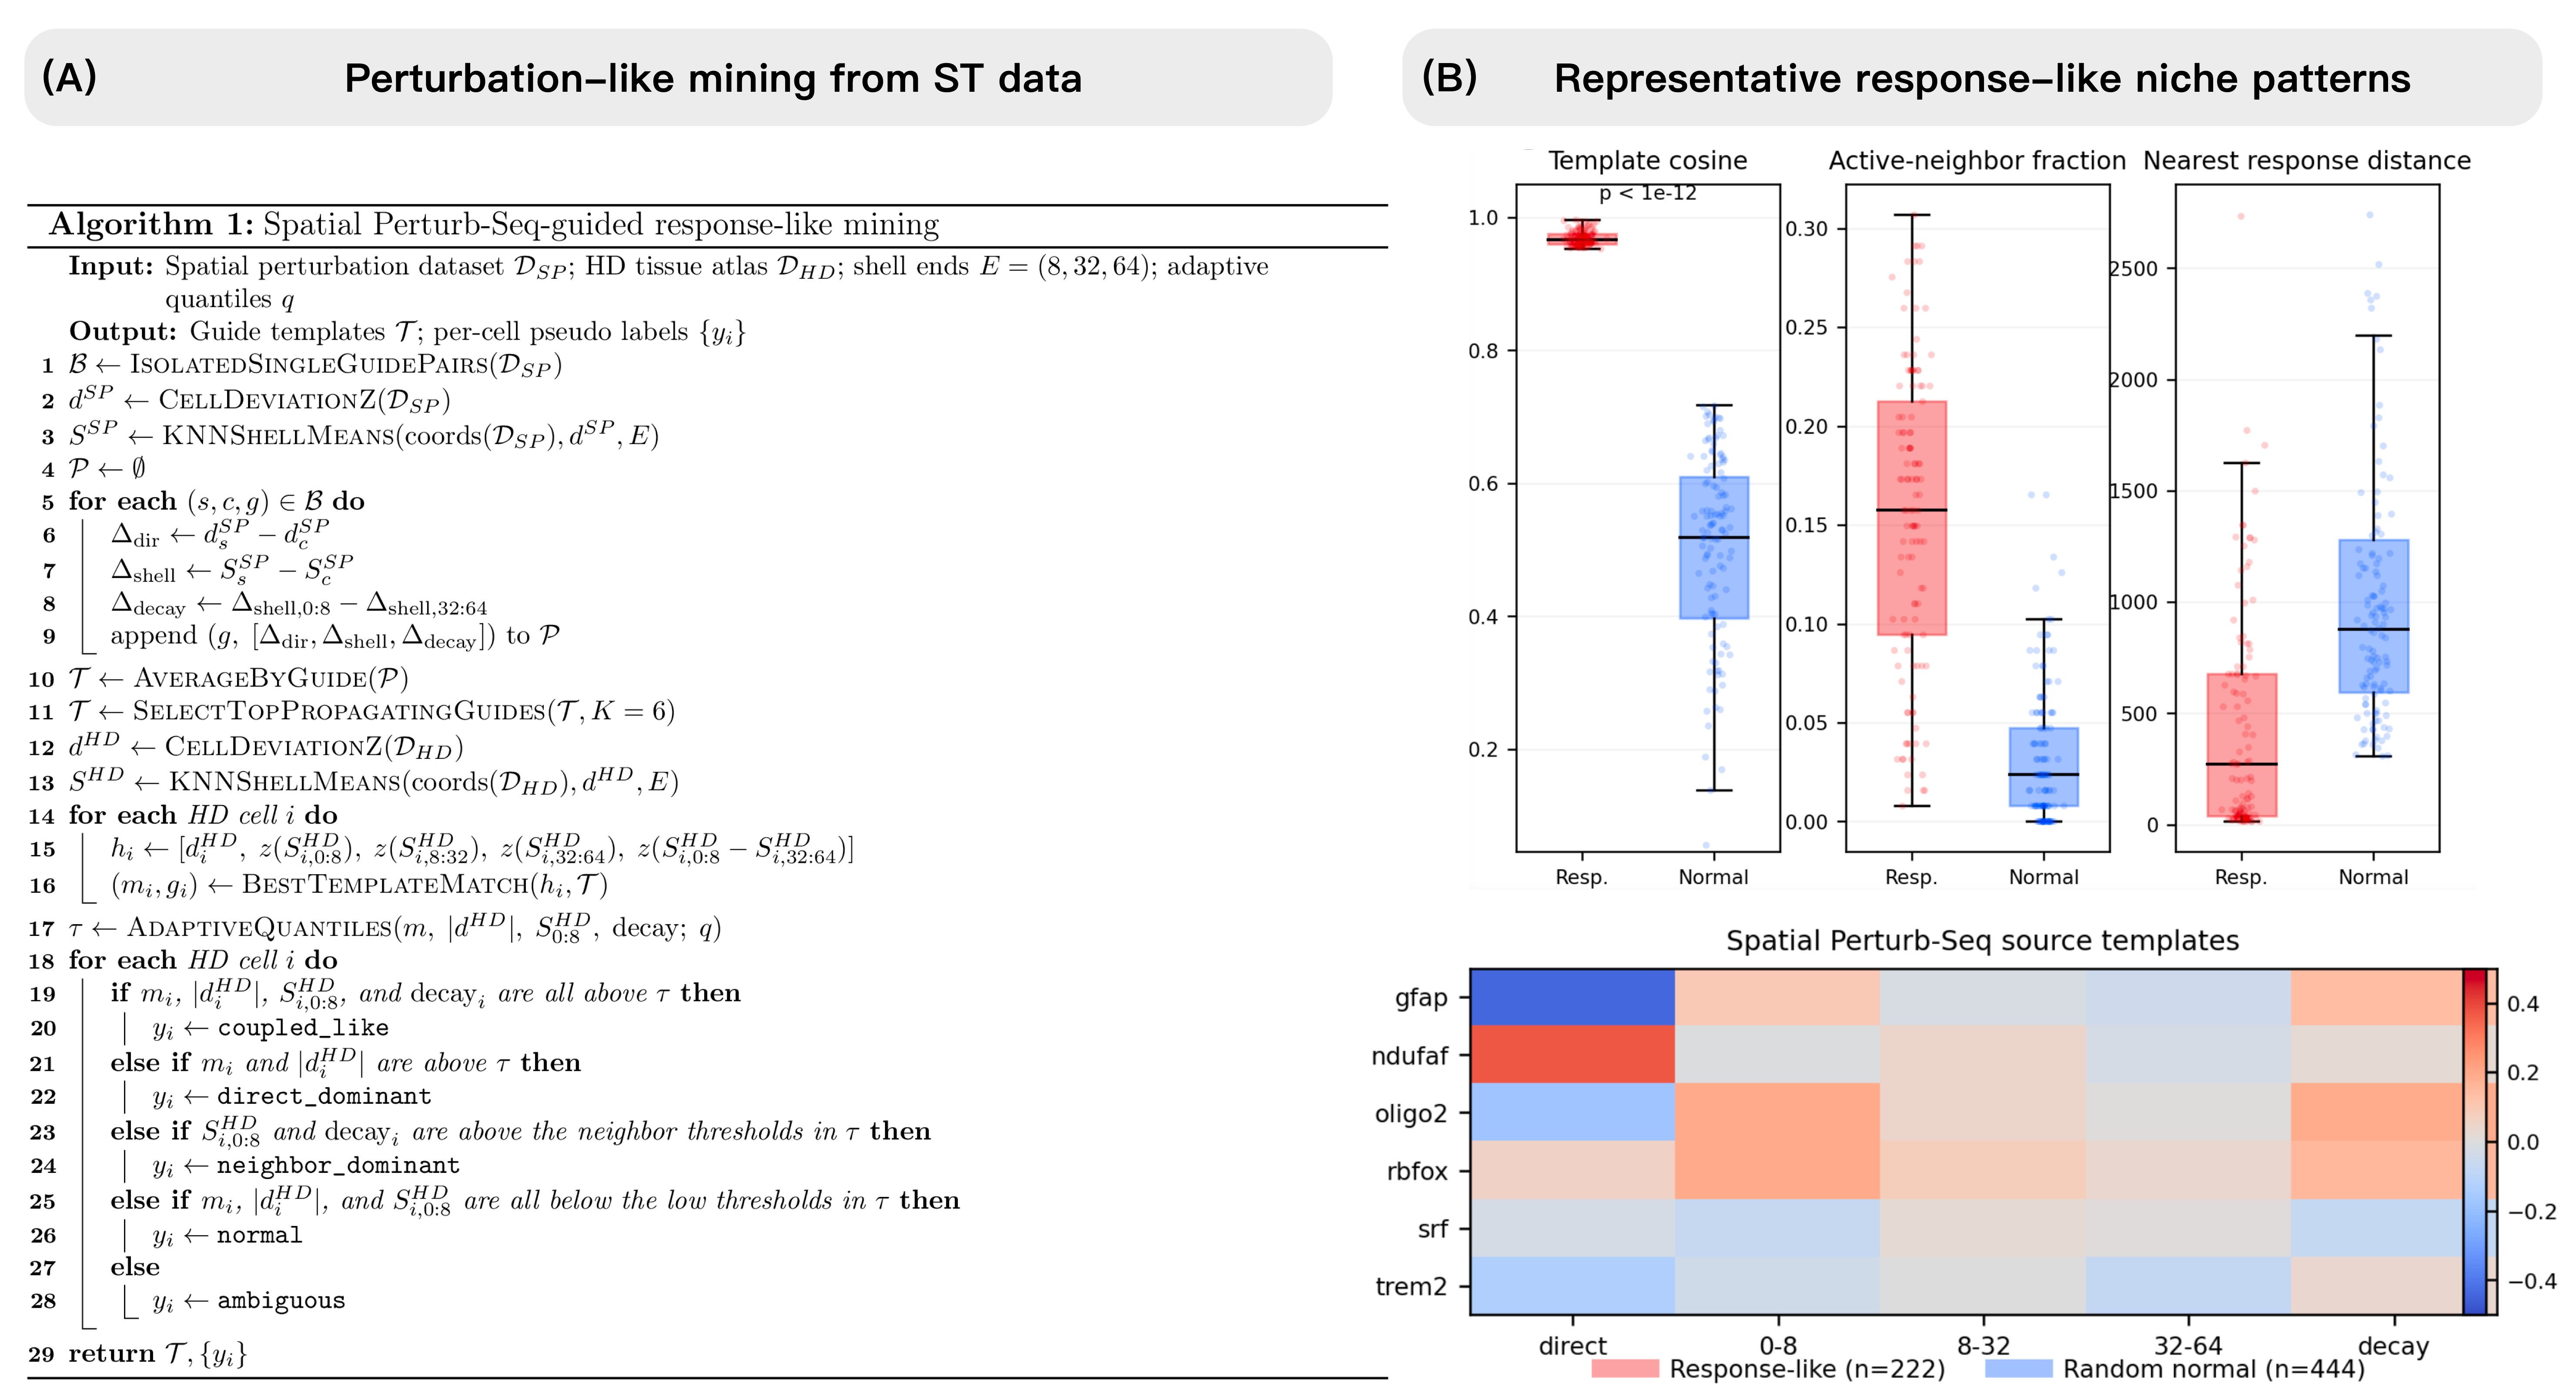
\includegraphics[width=0.82\textwidth]{TURB1.png}

\vspace{0.4em}

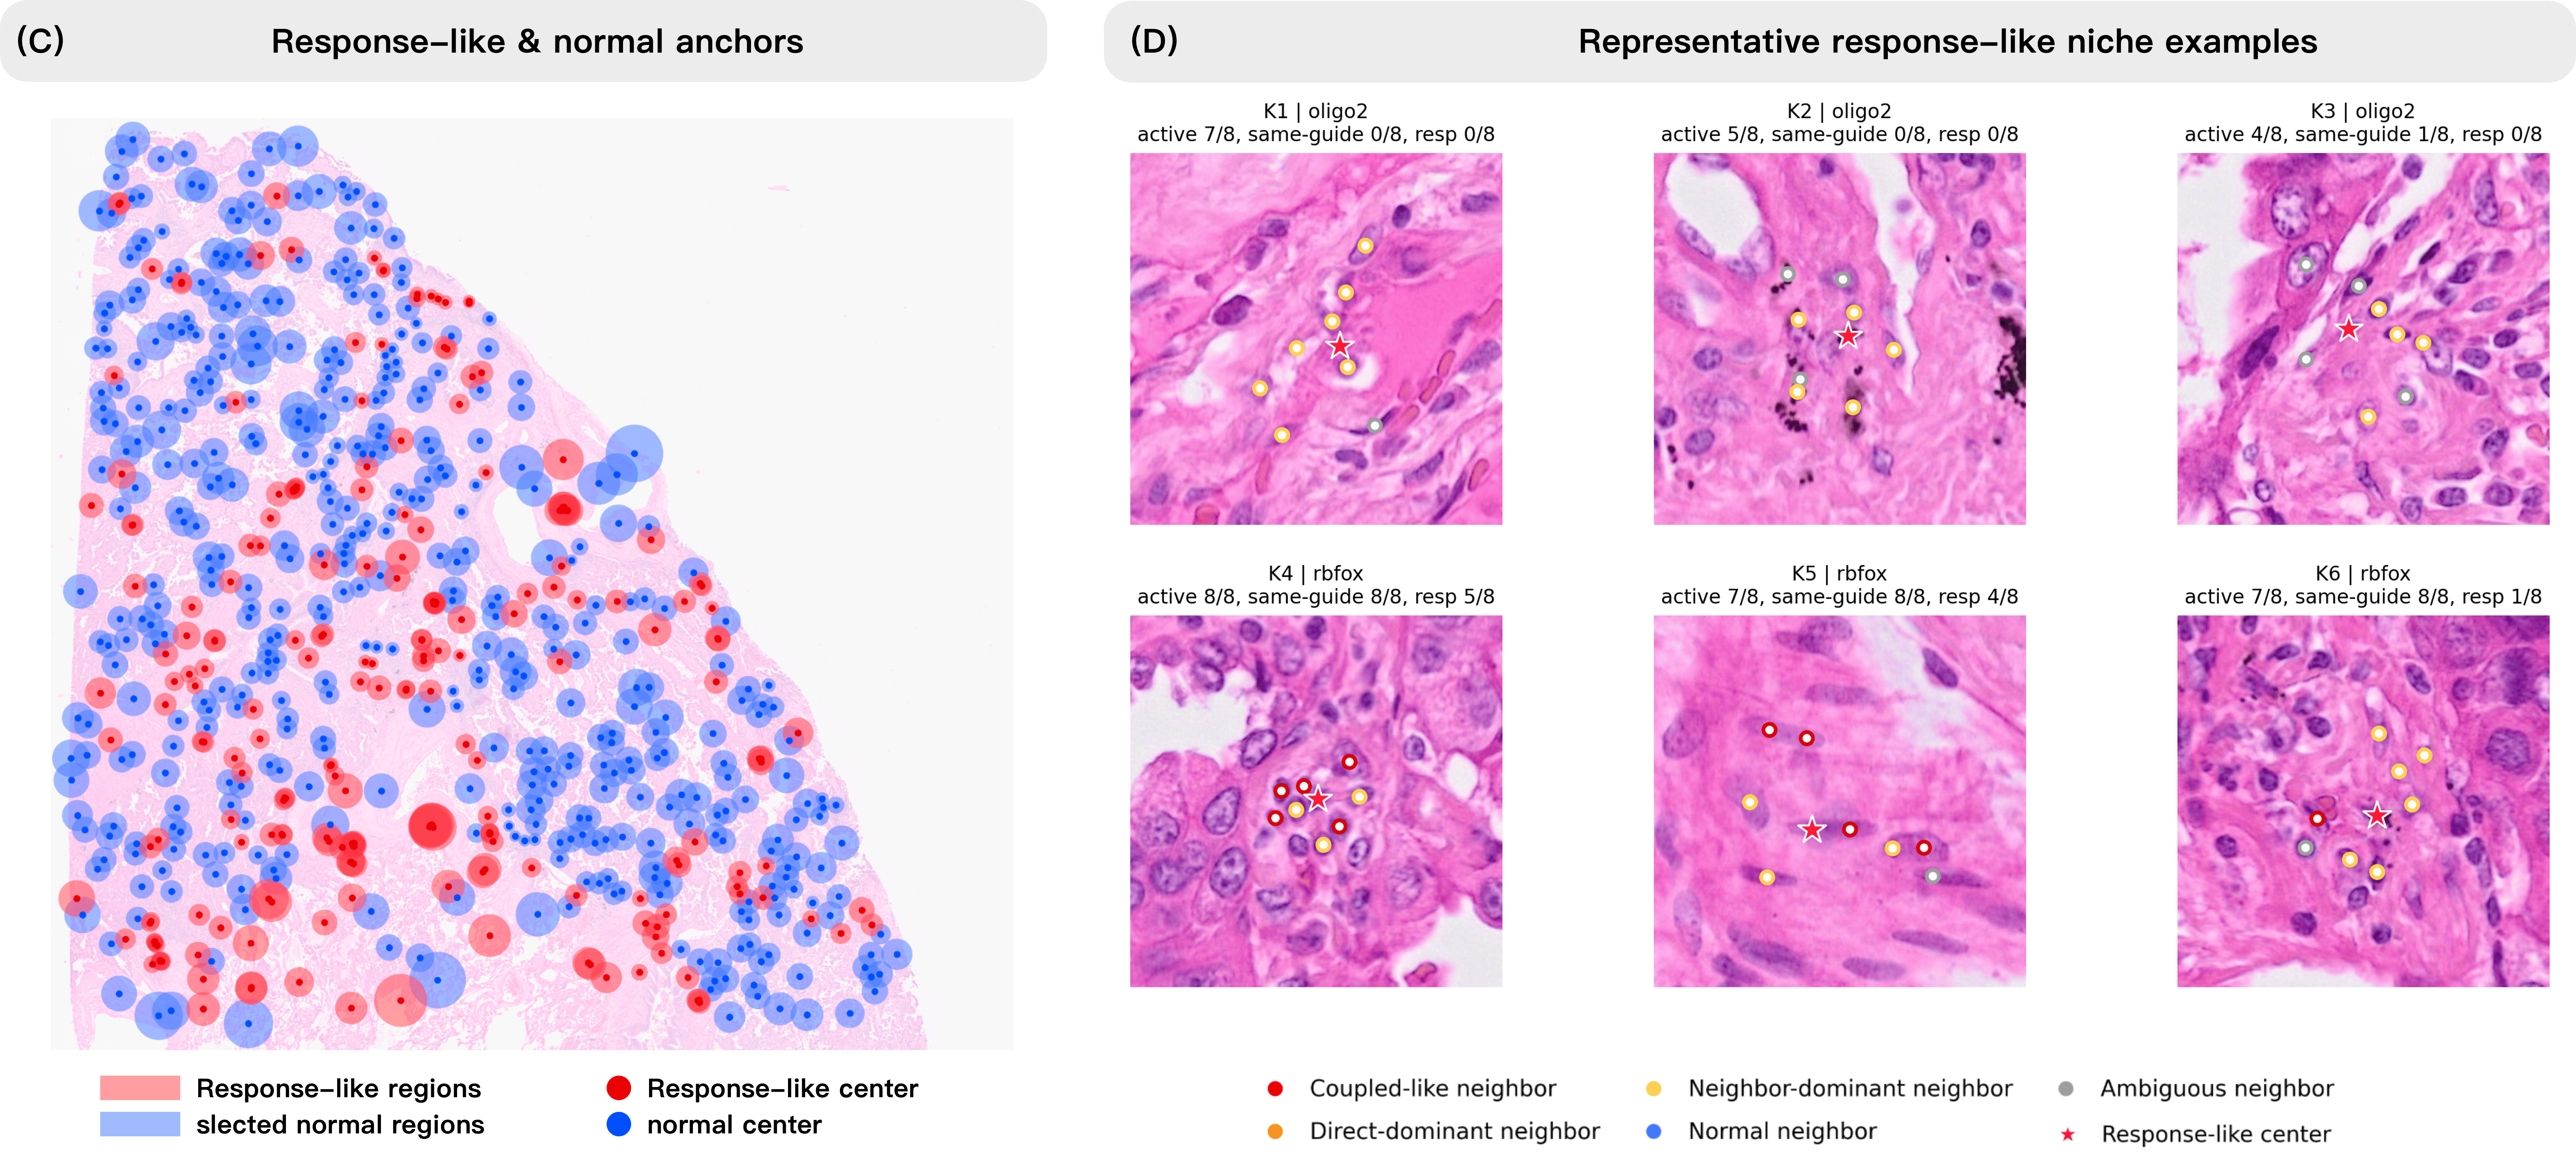
\includegraphics[width=0.82\textwidth]{TURB2.png}
\caption{Mining communication-rich microenvironments from unperturbed reference ST. Candidate tissue regions are scored for spatially local cell--cell structure, including neighborhood geometry, cell-state organization, and communication compatibility. Selected communication-rich and background regions pretrain a frozen reference microenvironment encoder without perturbation labels.}
\label{fig:app_st_mining}
\end{figure*}

\subsection{Communication-rich microenvironment mining}
\label{app:communication_microenvironment_mining}

\paragraph{Mining communication-rich microenvironments from unperturbed reference ST.}
The second data component uses unperturbed high-resolution spatial transcriptomics to identify reference microenvironments with strong local communication structure. These data are not used as perturbation labels. Instead, they provide spatial contexts in which cell--cell communication is plausible.

For each organ or tissue source, we construct a reference ST corpus
\[
\mathcal B=\{R_1,\ldots,R_N\},
\]
where each region $R$ contains local cells or spatial bins with expression profiles, coordinates, and inferred or annotated cell states. Within each region, we define a local cell--cell graph
\[
E_R=\{(i,j):\|s_i-s_j\|_2\le r,\ i\neq j\},
\]
where $r$ is a spatial interaction radius. A candidate communication program may correspond to a ligand--receptor pair, a ligand--target module, or a learned gene program. For a candidate gene pair or communication program $(p,q)$, the local communication score is
\[
\begin{aligned}
C_R(p,q)
&=
\frac{1}{|E_R|}
\sum_{(i,j)\in E_R}\tilde x_{ip}\tilde x_{jq}\\
&\quad \times
\exp\!\left(
-\frac{\|s_i-s_j\|_2^2}{2\sigma_d^2}
\right),
\end{aligned}
\]
where $\tilde x_{ip}$ and $\tilde x_{jq}$ are normalized expression values for the signal-side and response-side genes. This score favors regions where a signal-side program and a response-side program are jointly active in spatially adjacent cells.

Each region is summarized by its strongest communication programs and local tissue context:
\[
\begin{aligned}
h_R
&=
[\bar z_R,\pi_R,\mathrm{TopK}\{C_R(p,q)\},\rho_R],
\end{aligned}
\]
where $\bar z_R$ is the mean expression embedding, $\pi_R$ is the cell-type composition, and $\rho_R$ summarizes local spatial density and neighborhood geometry. Regions are selected as high-communication microenvironments if their communication scores exceed a reference-ST quantile threshold and both signal-side and response-side populations are sufficiently represented:
\[
\begin{aligned}
\mathcal R_{\mathrm{high}}
&=
\left\{
R\in\mathcal B:
\max_{(p,q)}C_R(p,q)\ge Q_{1-\eta},
\right.\\
&\qquad\left.
\ n_{\mathrm{signal}}(R)\ge n_{\min},
\ n_{\mathrm{response}}(R)\ge n_{\min}
\right\}.
\end{aligned}
\]
We also retain low-communication regions as background controls. Together, these regions form a reference library of communication-rich and communication-poor tissue contexts.

The mined regions are used to pretrain the reference microenvironment encoder. They expose the model to diverse local gene-coupling and cell--cell communication patterns, but do not define perturbation-response targets. During perturbation training, Spatial Perturb-Seq patches supervise the signed response field, while the frozen microenvironment encoder supplies niche context for ring-aware propagation refinement.

The corresponding reference communication prior is
\[
\begin{aligned}
A_{\mathrm{CCC}}(i,j)
&=
\sum_{(p,q)\in\mathcal G}
\beta_{pq}
\tilde x_{ip}\tilde x_{jq}\\
&\quad \times
\exp\!\left(
-\frac{\|s_i-s_j\|_2^2}{2\sigma_d^2}
\right),
\end{aligned}
\]
where $\mathcal G$ is the set of communication programs and $\beta_{pq}$ is a program weight learned from the mined regions. This prior acts as a gate for plausible communication paths. It does not define the perturbation target; effective propagated responses are still learned from true spatial perturbation supervision.

\subsection{Mouse perturbation-like microenvironment mining from HD and Xenium reference ST}
\label{app:mouse_microenvironment_mining}

To expand the reference microenvironment corpus beyond the single true spatial perturbation benchmark, we mined perturbation-like local regions from unperturbed mouse-brain HD and Xenium spatial transcriptomics datasets. These regions are not treated as perturbation-response labels. Instead, they provide diverse mouse-brain microenvironments in which specific gene programs are locally enriched and can be paired with matched background regions for reference-prior pretraining.

We used seven perturbation-like program templates spanning IFN/inflammatory, TREM2 microglia/DAM, astrocyte gliosis, myelin-lineage, neuronal/SRF, Rbfox/splicing, and mitochondrial/OXPHOS programs. Across two HD mouse-brain sections and three Xenium mouse-brain studies, this procedure screened 392,962 cells, identified 1,619 perturbation-like positive anchors, and generated 9,316 anchor--normal local pairs.

These mined anchor--normal pairs are used to pretrain the reference microenvironment encoder. The encoder learns local niche structure, program co-activation, and cell--cell plausibility from unperturbed reference ST. During supervised spatial perturbation training, however, the signed response targets still come only from Spatial Perturb-seq PPP pairs. Thus, the mined HD/Xenium regions mitigate the limited diversity of available ground-truth spatial perturbation data without converting unperturbed ST into pseudo perturbation labels.

\begin{figure}[t]
\centering
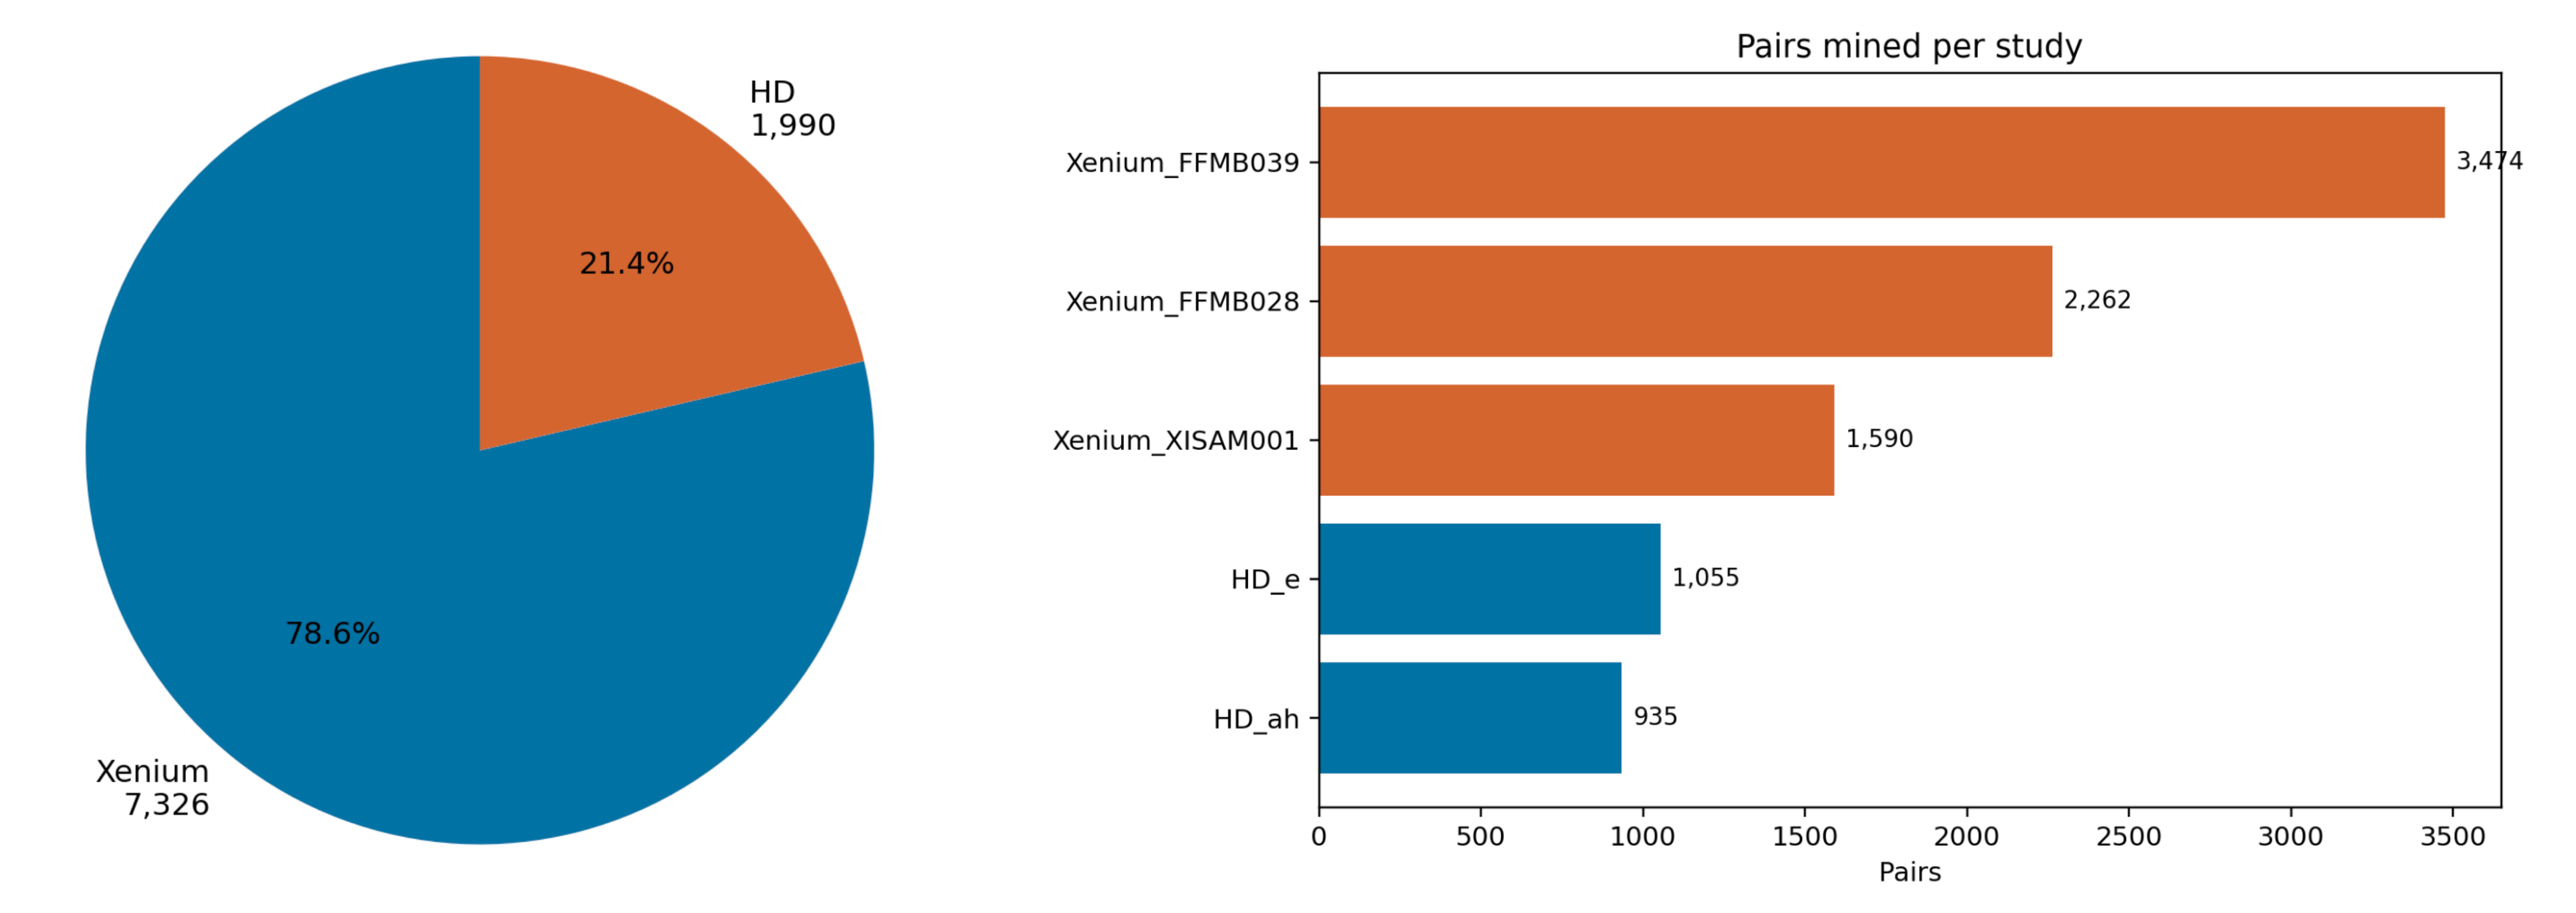
\includegraphics[width=\linewidth]{mouse_mining.png}
\vspace{-0.6em}
\caption{Mouse-brain perturbation-like microenvironment mining from HD and Xenium reference ST. Program-enriched local regions are identified from unperturbed mouse-brain spatial transcriptomics and paired with matched background regions. These mined pairs pretrain the frozen microenvironment prior used by \methodname{}, but do not define perturbation-response targets.}
\label{fig:mouse_mining}
\vspace{-0.6em}
\end{figure}

\paragraph{Study-level mining summary.}
The HD sections were dominated by Rbfox and OXPHOS-like anchors; \texttt{FFMB039} by myelin-like anchors; \texttt{FFMB028} by interferon and TREM2-like anchors; and \texttt{XISAM001} by neuronal/SRF and interferon-like anchors. Across all studies, the program totals were 587 myelin, 366 IFN/inflammatory, 238 Rbfox/splicing, 170 neuronal/SRF, 148 OXPHOS, 103 TREM2, and 7 astrocyte anchors.

\begin{table}[t]
\centering
\caption{Study-level mouse-brain microenvironment mining counts.}
\label{tab:mouse_mining_studies}
\footnotesize
\setlength{\tabcolsep}{3pt}
\renewcommand{\arraystretch}{1.10}
\begin{tabular}{@{}llrrr@{}}
\toprule
Study & Modality & Cells & Anchors & Pairs \\
\midrule

\texttt{HD\_e} & HD & 51,190 & 211 & 1,055 \\
\texttt{HD\_ah} & HD & 54,298 & 187 & 935 \\
\texttt{FFMB039} & Xenium & 162,033 & 579 & 3,474 \\
\texttt{FFMB028} & Xenium & 63,173 & 377 & 2,262 \\
\texttt{XISAM001} & Xenium & 62,268 & 265 & 1,590 \\

\midrule
Total & -- & 392,962 & 1,619 & 9,316 \\

\bottomrule
\end{tabular}
\end{table}

\subsection{Comparison to available spatial and single-cell perturbation resources}
\label{app:resource_comparison}

\begin{table}[t]
\centering
\caption{Resource support for cell-resolved propagation benchmarking.}
\label{tab:app_resource_comparison}
\scriptsize
\setlength{\tabcolsep}{2pt}
\renewcommand{\arraystretch}{1.18}
\begin{tabular}{@{}lcccccc@{}}
\toprule
\makecell[l]{Resource} &
\makecell[c]{SC} &
\makecell[c]{XY} &
\makecell[c]{Pert.} &
\makecell[c]{WT} &
\makecell[c]{Native} &
\makecell[c]{Ready} \\
\midrule
Spatial Perturb-Seq & Yes & Yes & Yes & Yes & Yes & Yes \\
Dissoc. perturb & Yes & No & Yes & Yes & No & No \\
Unperturbed ST & Part. & Yes & No & Part. & Yes & No \\
Perturb-map & Part. & Yes & Yes & Part. & Yes & No \\
Perturb-FISH & Yes & Yes & Yes & Targeted & Yes & No \\
Spatial CRISPR co-seq & Part. & Yes & Yes & Part./Yes & Yes & Not yet \\
Multi-condition ST & Part. & Yes & Cond. & Part. & Yes & No \\
\bottomrule
\end{tabular}
\end{table}

``Ready'' means that a public resource can directly define cell-resolved direct-effect-to-neighbor propagation targets with perturbation assignment, transcriptome-scale expression, and spatial coordinates measured in the same cells. Spatial Perturb-Seq is therefore the primary exact benchmark. Dissociated perturbation collections provide direct-effect priors but remove spatial neighborhoods. Unperturbed ST atlases provide tissue context without perturbation labels. Perturb-map and Perturb-FISH offer useful external support but lack matched whole-transcriptome cell-level neighbor-response fields in their current public forms. Emerging spatial CRISPR co-sequencing platforms are promising, but are not yet available as public benchmark-ready datasets for this task.

\subsection{Full method equations and training details}
\label{app:method_full_details}

\paragraph{Graph notation.}
Each local perturbation sample is a graph $P=(V,E)$ with $m=64$ cells. Cell $i$ has matched-control expression $x_i\in\mathbb R^G$, coarse cell state $c_i$, relative coordinate $p_i$, direct-effect-relative geometry $g_i$, direct-effect indicator $a_i\in\{0,1\}$, and direct-effect profile $d_i\in\mathbb R^G$. The direct-effect profile is nonzero only on direct-effect cells. Directed edge $(i,j)$ has features $e_{ij}$, including relative geometry, cell-type-pair indicators, and communication-compatibility score $q_{ij}$. The model predicts $\widehat\Delta_i\in\mathbb R^G$ and reconstructs $\widehat x_i^{\mathrm{post}}=x_i+\widehat\Delta_i$.

\paragraph{Niche-impact residualization.}
The response decomposition is
\[
\begin{aligned}
\Delta_i
&=
I_i^{\mathrm{niche}}+I_i^{\mathrm{prop}} .
\end{aligned}
\]
The niche module removes perturbation information:
\[
\begin{aligned}
\widehat I_i^{\mathrm{niche}}
&=
f_{\mathrm{niche}}(x,c,p,e;\ a=0,d=0).
\end{aligned}
\]
The propagation target is
\[
\begin{aligned}
I_i^{\mathrm{prop},\star}
&=
\Delta_i-\widehat I_i^{\mathrm{niche}} .
\end{aligned}
\]
Thus, matched-control variation, local tissue composition, and geometry are absorbed by $\widehat I_i^{\mathrm{niche}}$, while directed propagation learns perturbation-conditioned propagation impact.

\paragraph{Direct-effect and neighbor initialization.}
Each cell embedding is
\[
\begin{aligned}
h_i
&=
\phi_x(x_i)+\phi_c(c_i)+\phi_p(p_i)+\phi_g(g_i).
\end{aligned}
\]
Neighbor and direct-effect states are initialized separately:
\[
\begin{aligned}
n_i^0
&=\phi_N(h_i),\\
u_i^0
&=a_i\phi_D([h_i,d_i,g_i]).
\end{aligned}
\]
This construction prevents neighbor cells from directly seeing the perturbation input.

\paragraph{Directed direct-effect-to-neighbor propagation.}
For propagation layer $\ell$, a direct-effect-to-neighbor message from direct-effect cell $i$ to neighbor cell $j$ is
\[
\begin{aligned}
g_{ij}^{\ell}
&=
\sigma\!\left(
\phi_a([u_i^\ell,n_j^\ell,e_{ij}])
+
w_{\mathrm{comm}}q_{ij}
\right),
\end{aligned}
\]
\[
\begin{aligned}
\mu_{ij}^{\ell}
&=
g_{ij}^{\ell}
\phi_\mu([u_i^\ell,n_j^\ell,e_{ij}]).
\end{aligned}
\]
Neighbor messages are aggregated over direct-effect cells:
\[
\begin{aligned}
\bar\mu_j^\ell
&=
\sum_{i:a_i=1}\mu_{ij}^{\ell},\\
n_j^{\ell+1}
&=
\phi_u([n_j^\ell,\bar\mu_j^\ell]).
\end{aligned}
\]
After $L$ layers, the base propagation module predicts
\[
\begin{aligned}
\widehat I_i^{\mathrm{prop},\mathrm{base}}
&=
a_i\psi_{\mathrm{direct}}(u_i^L)
\\
&\quad +
(1-a_i)\psi_{\mathrm{neighbor}}(n_i^L).
\end{aligned}
\]

\paragraph{Reference-ST niche encoder.}
The reference encoder is pretrained on unperturbed ST regions and then frozen. It returns cell-level niche embeddings, a patch-level niche token, and edge-plausibility estimates:
\[
\begin{aligned}
&\{z_i^{\mathrm{ref}}\},\ n_P^{\mathrm{ref}},\\
&\qquad b_{ij}^{\mathrm{ref}},\ u_{ij}^{\mathrm{ref}}
 = f_{\mathrm{ref}}(x,c,p,e).
\end{aligned}
\]
The neighbor-side niche summary is
\[
\begin{aligned}
o_P
&=
\begin{bmatrix}
n_P^{\mathrm{ref}}\\
|V_N|^{-1}\sum_{j\in V_N}z_j^{\mathrm{ref}}
\end{bmatrix},
\end{aligned}
\]
where $V_N$ is the neighbor set. The frozen reference context is injected through zero-initialized adapters:
\[
\begin{aligned}
u_i^0
&\leftarrow
u_i^0+a_i\lambda_D\phi_D^{\mathrm{ref}}(o_P),\\
n_i^0
&\leftarrow
n_i^0+(1-a_i)\lambda_N\phi_N^{\mathrm{ref}}(o_P).
\end{aligned}
\]
Because $\lambda_D$ and $\lambda_N$ are initialized at zero, the reference-ST module begins as the base propagation model and learns only microenvironment corrections.

\paragraph{Ring-aware response feedback.}
The ST-conditioned module first predicts $\widehat I_i^{\mathrm{prop},(1)}$. Neighbor response strength is scored by
\[
\kappa_j
=
\frac{1}{G}
\sum_{g=1}^{G}
\left|
\widehat I_{jg}^{\mathrm{prop},(1)}
\right|.
\]
The top 5\% neighbor cells by $\kappa_j$ are selected as feedback cells $F$. Neighbors are partitioned by direct-effect-relative distance into three rings: nearest eight neighbors, next 24 neighbors, and remaining neighbors. For each ring $b$, the model constructs a response token:
\[
\begin{aligned}
t_b
&=
\phi_b\!\left(
\begin{bmatrix}
\mathrm{mean}_{j\in F\cap B_b}\widehat I_j^{\mathrm{prop},(1)}\\
\mathrm{std}_{j\in F\cap B_b}\widehat I_j^{\mathrm{prop},(1)}
\end{bmatrix}
\right).
\end{aligned}
\]
The direct-effect cells receive the average ring token, and each neighbor receives the token for its ring. A second directed propagation pass produces $\widehat I_i^{\mathrm{prop},(2)}$.

\paragraph{Restricted ring-aware correction.}
The final ST-conditioned propagation impact is
\[
\begin{aligned}
\widehat I_i^{\mathrm{prop},\mathrm{st}}
&=
\widehat I_i^{\mathrm{prop},(1)}
+
\lambda_i
\mathbf 1[i\in V_D\cup F]
\left(
\widehat I_i^{\mathrm{prop},(2)}-\widehat I_i^{\mathrm{prop},(1)}
\right),
\end{aligned}
\]
where $V_D$ is the direct-effect set, $F$ is the feedback-neighbor set, and neighbor-side $\lambda_i$ is ring-specific. This restriction lets high-response regions feed back into the model without allowing the second pass to uniformly rewrite all neighbor cells.

\paragraph{Final response prediction.}
The final prediction is
\[
\begin{aligned}
\widehat\Delta_i
&=
\widehat I_i^{\mathrm{niche}}
+
(1-\alpha)\widehat I_i^{\mathrm{prop},\mathrm{base}}
\\
&\quad +
\alpha\widehat I_i^{\mathrm{prop},\mathrm{st}},
\end{aligned}
\]
with $\alpha=0.65$ selected on validation data. This is a propagation-delta blend. The reconstructed post-state expression is
\[
\widehat x_i^{\mathrm{post}}
=
x_i+\widehat\Delta_i.
\]

\paragraph{Reference-ST pretraining objective.}
The reference microenvironment encoder is trained without perturbation labels:
\[
\begin{aligned}
\mathcal L_{\mathrm{ref}}
&=
2.0\mathcal L_{\mathrm{masked\text{-}program}}
+
1.0\mathcal L_{\mathrm{neighborhood}}
\\
&\quad +
0.25\mathcal L_{\mathrm{patch\text{-}hist}}
+
0.25\mathcal L_{\mathrm{edge}}.
\end{aligned}
\]
The terms supervise masked gene-program reconstruction, neighborhood-conditioned program prediction, patch cell-type composition, and pseudo edge-plausibility prediction. These objectives teach local niche structure and communication plausibility, but not perturbation response.

\paragraph{Propagation-impact objective.}
After niche-impact residualization, the propagation module is trained with neighbor-focused supervision:
\[
\begin{aligned}
\mathcal L_{\mathrm{prop}}
&=
1.0\mathcal L_{\mathrm{neighbor}}
+
0.3\mathcal L_{\mathrm{ring}}
\\
&\quad +
0.3\mathcal L_{\mathrm{post}}
+
0.1\mathcal L_{\mathrm{rank}}.
\end{aligned}
\]
$\mathcal L_{\mathrm{neighbor}}$ is a Huber loss on high-confidence neighbor-cell propagation impacts. $\mathcal L_{\mathrm{ring}}$ supervises ring-aggregated response after adding the niche-impact baseline. $\mathcal L_{\mathrm{post}}$ supervises reconstructed post-state expression $x_i+\widehat I_i^{\mathrm{niche}}+\widehat I_i^{\mathrm{prop}}$. $\mathcal L_{\mathrm{rank}}$ is a pairwise ranking loss over per-patch gene-response magnitudes. The direct-effect-cell loss weight is set to zero in the strongest propagation setting so that the easier direct-effect signal does not dominate neighbor propagation.

\subsection{Full gene-centric neighbor-response validation}
\label{app:full_gene_centric_validation}


\subsection{Strict grouped guide-out stability}
\label{sec:guide_stratified_stability}
\label{app:strict_guide_ood}

To test perturbation-level generalization, we use a strict grouped guide-out split. The perturbation guides \textit{fasn}, \textit{stk39}, and \textit{trem2} are jointly excluded from training and validation, yielding 992 unseen-guide graphs. With observed sender-side direct-effect seeds, \methodname{} reaches pooled neighbor/ring Pearson $0.596/0.451$, outperforming elastic-net patch-summary regression $(0.334/0.142)$ and a Generic Graph Transformer without CCC priors $(0.497/0.395)$. Per-guide performance remains stable across all three held-out perturbations, indicating that the grouped guide-out result is not driven by a single guide.

\begin{table*}[t]
\centering
\footnotesize
\setlength{\tabcolsep}{4pt}
\renewcommand{\arraystretch}{1.04}
\caption{\textbf{Strict grouped guide-out evaluation.}
The perturbation guides \textit{fasn}, \textit{stk39}, and \textit{trem2} are held out jointly during training and validation. The table reports per-guide performance for \methodname{} under observed and zero direct-effect seeds, together with exact-task baseline performance on the same unseen-guide graphs. Neighbor, centered, and ring scores are Pearson correlations.}
\label{tab:strict_grouped_guide_out}
\resizebox{\linewidth}{!}{%
\begin{tabular}{llrcccc}
\toprule
\textbf{Model} &
\textbf{Held-out guide} &
\textbf{$n$ graphs} &
\textbf{Input} &
\textbf{Neighbor} &
\textbf{Centered} &
\textbf{Ring} \\
\midrule

\rowcolor{gray!12}
\multicolumn{7}{l}{\textit{\methodname{} on the strict grouped guide-out split.}} \\

\methodname{} &
\textit{fasn} &
413 &
Observed seed &
0.5982 &
\textemdash &
0.4540 \\

\methodname{} &
\textit{stk39} &
351 &
Observed seed &
0.5978 &
\textemdash &
0.4573 \\

\methodname{} &
\textit{trem2} &
228 &
Observed seed &
0.6006 &
\textemdash &
0.4562 \\

\methodname{} &
Overall &
992 &
Observed seed &
0.5964 &
\textemdash &
0.4514 \\

\addlinespace[1pt]
\methodname{} &
\textit{fasn} &
413 &
Zero seed &
0.5983 &
\textemdash &
0.4449 \\

\methodname{} &
\textit{stk39} &
351 &
Zero seed &
0.5979 &
\textemdash &
0.4466 \\

\methodname{} &
\textit{trem2} &
228 &
Zero seed &
0.6013 &
\textemdash &
0.4517 \\

\methodname{} &
Overall &
992 &
Zero seed &
0.5964 &
\textemdash &
0.4374 \\

\midrule
\rowcolor{gray!12}
\multicolumn{7}{l}{\textit{Exact-task baselines on the same unseen-guide graphs.}} \\

Elastic-net patch-summary &
\textit{fasn} &
413 &
Patch summary &
0.3345 &
0.4820 &
0.1376 \\

Elastic-net patch-summary &
\textit{stk39} &
351 &
Patch summary &
0.3352 &
0.4838 &
0.1366 \\

Elastic-net patch-summary &
\textit{trem2} &
228 &
Patch summary &
0.3398 &
0.4856 &
0.1393 \\

Generic Graph Transformer, no CCC &
\textit{fasn} &
413 &
Graph only &
0.4991 &
0.5121 &
0.3918 \\

Generic Graph Transformer, no CCC &
\textit{stk39} &
351 &
Graph only &
0.4984 &
0.5120 &
0.3956 \\

Generic Graph Transformer, no CCC &
\textit{trem2} &
228 &
Graph only &
0.5009 &
0.5148 &
0.3887 \\

\bottomrule
\end{tabular}
}
\end{table*}

The \methodname{} rows are consistent across the three unseen perturbations: observed-seed neighbor Pearson stays between $0.5978$ and $0.6006$, and observed-seed ring Pearson stays between $0.4540$ and $0.4573$. Zero-seed evaluation preserves nearly identical neighbor Pearson but reduces ring Pearson to $0.4449$--$0.4517$. The two baseline families remain substantially lower in ring Pearson across all three guides, supporting strict grouped guide-out generalization rather than a single-guide artifact.

\subsection{Guide-stratified stability on the held-out Spatial Perturb-Seq test set}
\label{app:guide_stratified_stability}

To test whether the held-out Spatial Perturb-Seq result is dominated by a small
number of perturbation guides, we stratified the frozen \methodname{} predictions
by guide identity on the held-out test split. This is a guide-stratified stability
audit of the same held-out test predictions, not a leave-one-guide-out retraining
experiment. We include guides with at least 20 held-out test patches.

Across 14 guides, performance is stable and closely matches the overall test result.
The overall held-out split reaches neighbor/ring Pearson $0.6842/0.4574$ over
928 patches. The mean across guide strata is $0.6851 \pm 0.0044$ for neighbor
Pearson and $0.4604 \pm 0.0203$ for ring Pearson. Per-guide neighbor Pearson ranges
from $0.6767$ to $0.6952$, and per-guide ring Pearson ranges from $0.4276$ to
$0.4956$. This indicates that the aggregate held-out performance is not driven by
a single guide or a small subset of guides.

\begin{figure}[t]
    \centering
    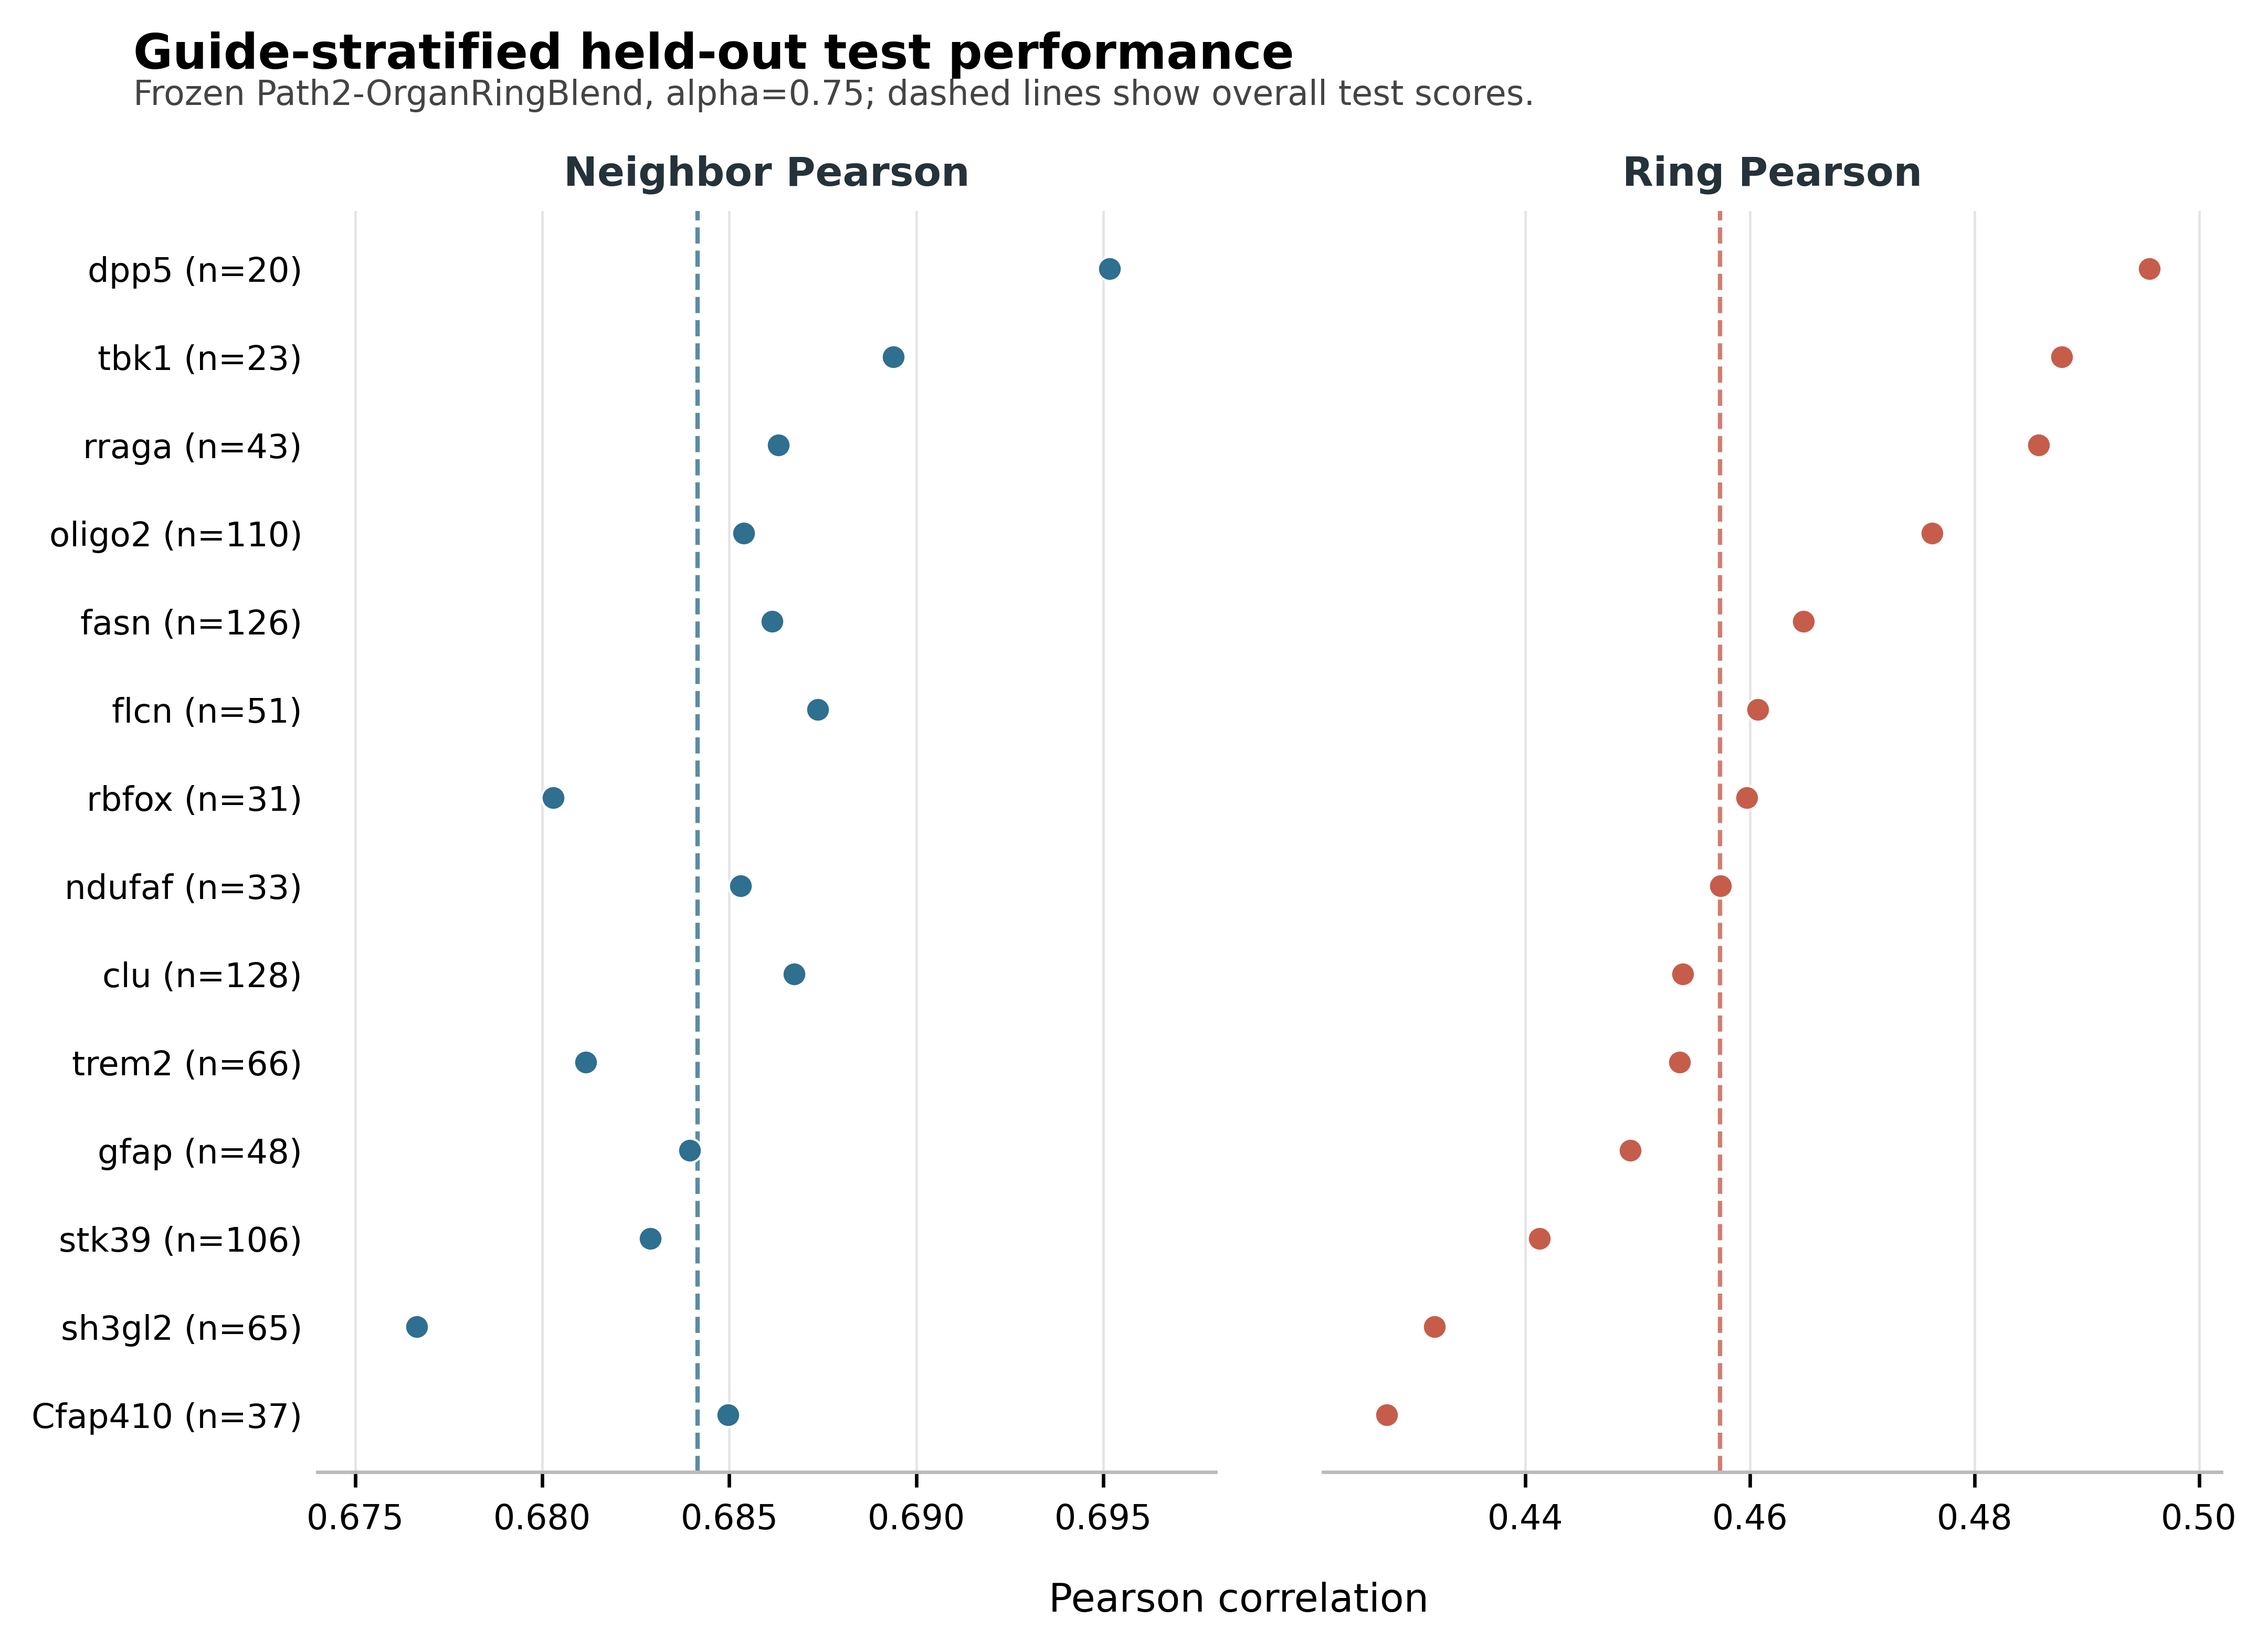
\includegraphics[width=1.0\linewidth]{path2_organringblend_guide_stratified_heldout_test_dotplot.png}
    \caption{\textbf{Guide-stratified held-out test stability.}
    Frozen \methodname{} predictions are stratified by guide identity on the same
    held-out Spatial Perturb-Seq test split. Dashed vertical lines show the overall
    held-out test scores. Across 14 guides with at least 20 test patches, both
    neighbor and ring Pearson remain close to the overall result, indicating that
    the benchmark performance is not driven by a small number of guides.}
    \label{fig:guide_stratified_stability}
\end{figure}

\begin{table}[t]
\centering
\footnotesize
\setlength{\tabcolsep}{5pt}
\renewcommand{\arraystretch}{1.06}
\caption{\textbf{Guide-stratified held-out test performance.}
The first two rows summarize the overall test split and the mean across guide strata.
Per-guide rows include guides with at least 20 held-out test patches.}
\label{tab:guide_stratified_stability}
\begin{tabular}{lccc}
\toprule
\textbf{Readout} & \textbf{Test patches} & \textbf{Neighbor Pearson} & \textbf{Ring Pearson} \\
\midrule
Overall test split & 928 & 0.6842 & 0.4574 \\
Mean across guides & 887 & $0.6851 \pm 0.0044$ & $0.4604 \pm 0.0203$ \\
\midrule
\textit{clu} & 128 & 0.6867 & 0.4540 \\
\textit{fasn} & 126 & 0.6861 & 0.4648 \\
\textit{oligo2} & 110 & 0.6854 & 0.4762 \\
\textit{stk39} & 106 & 0.6829 & 0.4413 \\
\textit{trem2} & 66 & 0.6812 & 0.4537 \\
\textit{sh3gl2} & 65 & 0.6767 & 0.4319 \\
\textit{flcn} & 51 & 0.6874 & 0.4607 \\
\textit{gfap} & 48 & 0.6839 & 0.4493 \\
\textit{rraga} & 43 & 0.6863 & 0.4857 \\
\textit{Cfap410} & 37 & 0.6850 & 0.4276 \\
\textit{ndufaf} & 33 & 0.6853 & 0.4574 \\
\textit{rbfox} & 31 & 0.6803 & 0.4597 \\
\textit{tbk1} & 23 & 0.6894 & 0.4878 \\
\textit{dpp5} & 20 & 0.6952 & 0.4956 \\
\bottomrule
\end{tabular}
\end{table}

% If not already defined:
% \newcommand{\pmv}[2]{#1\,{\scriptsize$\pm$}\,#2}

\begin{figure*}[t]
\centering
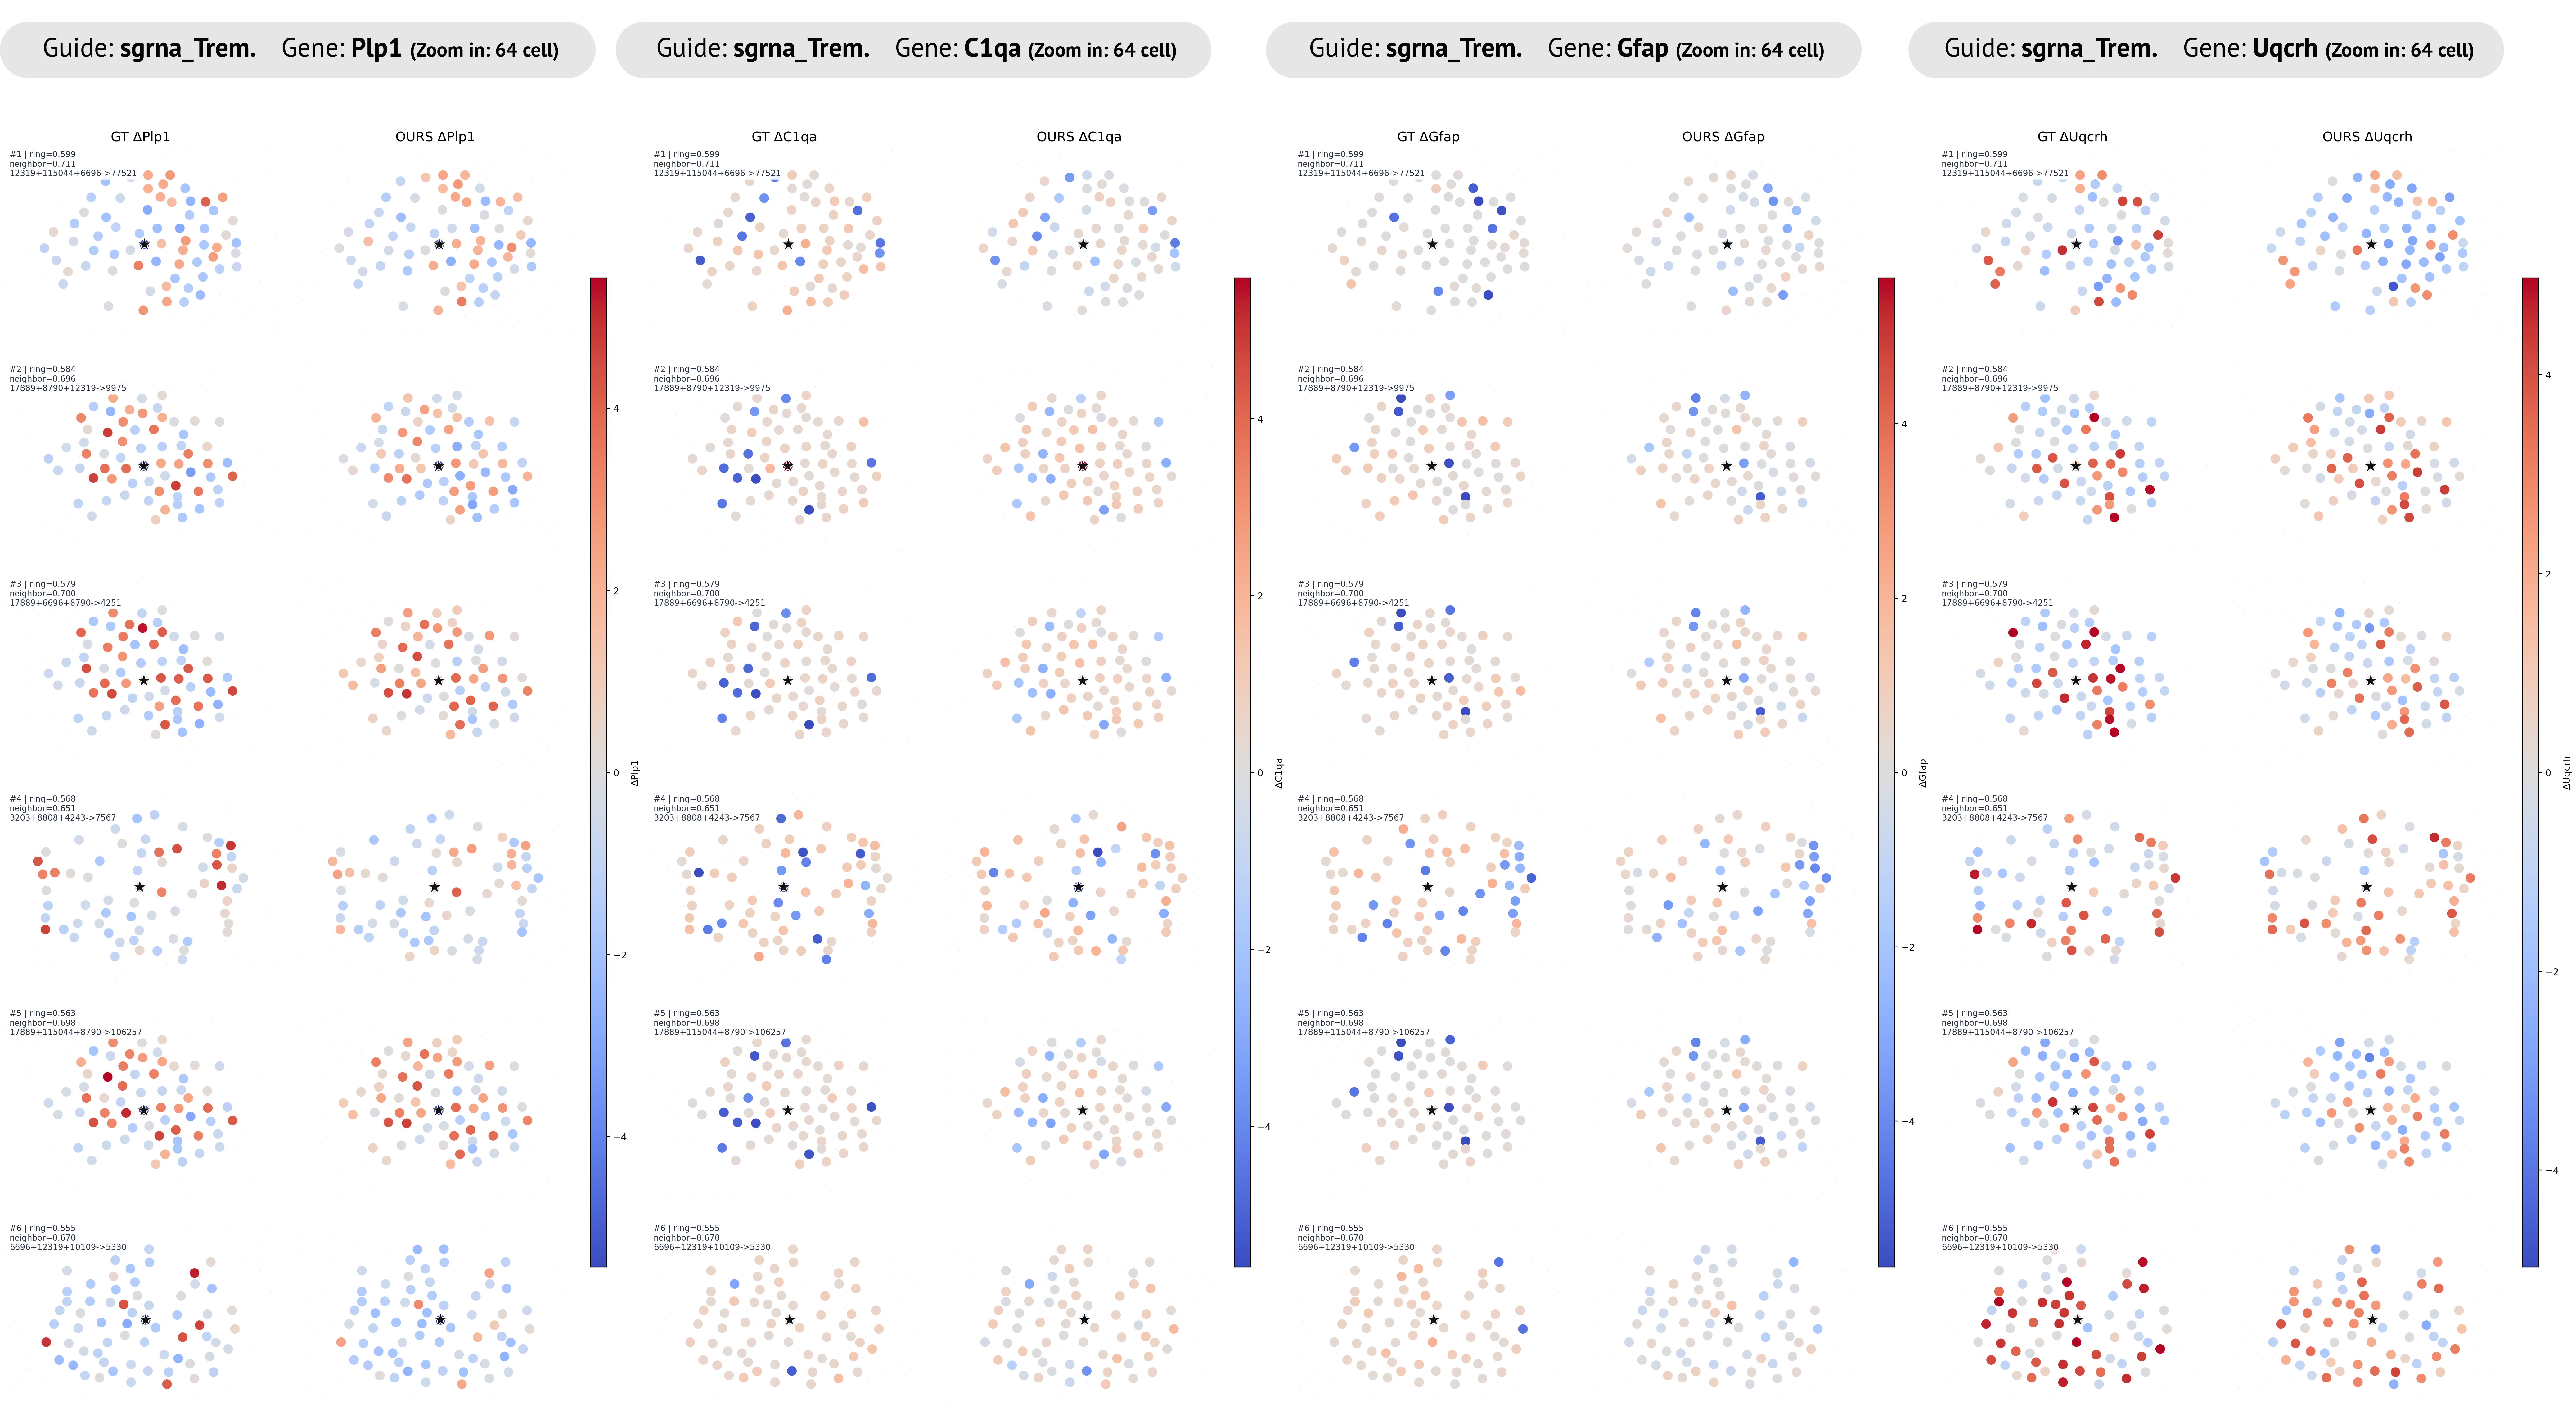
\includegraphics[width=0.98\linewidth]{main_result.png}
\caption{\textbf{Expanded real-data validation results on the Spatial Perturb-Seq mouse-brain benchmark.}
This appendix figure provides the full-resolution version of the main real-data evaluation summarized in \Cref{fig:main_exp}, including spatial response maps, local neighbor-cell neighborhoods, and gene-level recovery patterns under the block-held-out matched-control setting.}
\label{fig:app_main_result}
\end{figure*}

\begin{table*}[t]
\centering
\footnotesize
\setlength{\tabcolsep}{3.2pt}
\renewcommand{\arraystretch}{1.02}
\caption{\textbf{Full gene-centric neighbor-cell performance on the Spatial Perturb-Seq benchmark.}
Values are computed over neighbor cells and reported as estimate with uncertainty.
Gray rows mark perturbation-related, high-variance, and high-change gene groups.}
\label{tab:app_validation_summary}
\resizebox{\linewidth}{!}{%
\begin{tabular}{@{}lcccccccc@{}}
\toprule
\textbf{Gene} &
\textbf{Mean $|\Delta|$} &
\textbf{Pearson} &
\textbf{Spearman} &
\textbf{Cosine} &
\textbf{$R^2$} &
\textbf{MAE} &
\textbf{RMSE} &
\textbf{Sign acc.} \\
\midrule

\rowcolor{gray!18}
\multicolumn{9}{@{}l}{\textbf{\textit{Perturbation-related genes.}}} \\
\textit{Gfap}   & \pmv{0.966}{0.016} & \pmv{0.788}{0.005} & \pmv{0.313}{0.013} & \pmv{0.788}{0.005} & \pmv{0.621}{0.007} & \pmv{0.785}{0.008} & \pmv{1.047}{0.011} & \pmv{0.716}{0.007} \\
\textit{Trem2}  & \pmv{0.324}{0.006} & \pmv{0.266}{0.005} & \pmv{0.053}{0.012} & \pmv{0.243}{0.005} & \pmv{0.047}{0.004} & \pmv{0.449}{0.005} & \pmv{0.968}{0.010} & \pmv{0.586}{0.009} \\
\textit{C1qa}   & \pmv{0.996}{0.012} & \pmv{0.835}{0.003} & \pmv{0.309}{0.009} & \pmv{0.835}{0.003} & \pmv{0.694}{0.005} & \pmv{0.690}{0.005} & \pmv{0.916}{0.007} & \pmv{0.788}{0.004} \\
\textit{Olig2}  & \pmv{0.287}{0.007} & \pmv{0.184}{0.006} & \pmv{-0.004}{0.012} & \pmv{0.180}{0.004} & \pmv{0.018}{0.004} & \pmv{0.385}{0.005} & \pmv{0.865}{0.011} & \pmv{0.546}{0.010} \\
\textit{Opalin} & \pmv{0.868}{0.014} & \pmv{0.781}{0.003} & \pmv{0.383}{0.012} & \pmv{0.775}{0.003} & \pmv{0.601}{0.006} & \pmv{0.722}{0.006} & \pmv{0.991}{0.008} & \pmv{0.652}{0.007} \\

\midrule
\rowcolor{gray!18}
\multicolumn{9}{@{}l}{\textbf{\textit{Top five high-variance genes.}}} \\
\textit{Ptgds}  & \pmv{1.984}{0.010} & \pmv{0.805}{0.004} & \pmv{0.810}{0.004} & \pmv{0.805}{0.004} & \pmv{0.645}{0.007} & \pmv{1.087}{0.011} & \pmv{1.382}{0.014} & \pmv{0.913}{0.003} \\
\textit{Plp1}   & \pmv{1.743}{0.014} & \pmv{0.737}{0.005} & \pmv{0.745}{0.006} & \pmv{0.737}{0.005} & \pmv{0.533}{0.009} & \pmv{1.174}{0.013} & \pmv{1.501}{0.016} & \pmv{0.807}{0.004} \\
\textit{Ywhaz}  & \pmv{2.020}{0.010} & \pmv{0.772}{0.005} & \pmv{0.776}{0.005} & \pmv{0.759}{0.005} & \pmv{0.540}{0.011} & \pmv{1.274}{0.017} & \pmv{1.588}{0.019} & \pmv{0.898}{0.003} \\
\textit{Uqcrh}  & \pmv{1.971}{0.010} & \pmv{0.790}{0.004} & \pmv{0.773}{0.005} & \pmv{0.788}{0.004} & \pmv{0.616}{0.008} & \pmv{1.123}{0.012} & \pmv{1.416}{0.015} & \pmv{0.894}{0.003} \\
\textit{Sst}    & \pmv{2.031}{0.014} & \pmv{0.773}{0.006} & \pmv{0.733}{0.007} & \pmv{0.770}{0.006} & \pmv{0.580}{0.011} & \pmv{1.245}{0.019} & \pmv{1.581}{0.024} & \pmv{0.862}{0.006} \\

\midrule
\rowcolor{gray!18}
\multicolumn{9}{@{}l}{\textbf{\textit{High-change genes.}}} \\
\textit{Cycs}   & \pmv{2.356}{0.015} & \pmv{0.851}{0.003} & \pmv{0.693}{0.007} & \pmv{0.843}{0.004} & \pmv{0.708}{0.007} & \pmv{1.161}{0.014} & \pmv{1.462}{0.018} & \pmv{0.923}{0.003} \\
\textit{Nme2}   & \pmv{2.347}{0.014} & \pmv{0.874}{0.002} & \pmv{0.714}{0.005} & \pmv{0.873}{0.002} & \pmv{0.762}{0.004} & \pmv{1.051}{0.010} & \pmv{1.328}{0.012} & \pmv{0.951}{0.002} \\
\textit{Rack1}  & \pmv{2.333}{0.011} & \pmv{0.880}{0.002} & \pmv{0.678}{0.006} & \pmv{0.872}{0.003} & \pmv{0.759}{0.005} & \pmv{1.056}{0.011} & \pmv{1.332}{0.014} & \pmv{0.928}{0.003} \\
\textit{Ptma}   & \pmv{2.203}{0.012} & \pmv{0.882}{0.002} & \pmv{0.678}{0.005} & \pmv{0.878}{0.002} & \pmv{0.769}{0.004} & \pmv{1.008}{0.010} & \pmv{1.265}{0.012} & \pmv{0.966}{0.002} \\
\textit{Psmb4}  & \pmv{2.197}{0.008} & \pmv{0.826}{0.004} & \pmv{0.810}{0.004} & \pmv{0.826}{0.004} & \pmv{0.673}{0.007} & \pmv{1.132}{0.013} & \pmv{1.421}{0.015} & \pmv{0.926}{0.003} \\

\bottomrule
\end{tabular}
}
\end{table*}

% =========================================================
% Appendix: Controlled synthetic LR-propagation benchmark
% Required packages:
% \usepackage{booktabs}
% \usepackage{graphicx}
% \usepackage{subcaption}
% \usepackage{array}
% =========================================================

\subsection{Controlled synthetic LR-propagation validation}
\label{app:synthetic_lr_validation}

To complement the exact cell-resolved Spatial Perturb-Seq benchmark, we constructed
a controlled synthetic LR-propagation benchmark using external in vivo mouse
Perturb-seq direct-effect signatures from Jin \textit{et al.} (GSE157977), unperturbed
mouse-brain spatial graphs, and a NicheNet/LR-based neighbor-response simulator.
This setting is not biological ground truth; it is a controlled validation benchmark
for testing whether direct-effect-conditioned neighbor propagation is learnable when the
response field is generated under known communication rules.

The main synthetic split contains 432 graphs, with 252/72/108 train/validation/test
graphs. Random, clustered, and interface direct-effect geometries are balanced across
splits, as are perturbation strengths $0.75$, $1.25$, and $2.0$. We report
Neighbor Pearson and ring-level Pearson as the primary readouts. Niche-module-only
predictions are near zero, indicating that the synthetic target is not explained by
tissue context alone. Synthetic fine-tuning recovers the held-out response field,
whereas direct transfer from the real-data pretrained model remains weak, consistent
with simulator-distribution mismatch.

\begin{figure*}[t]
    \centering
    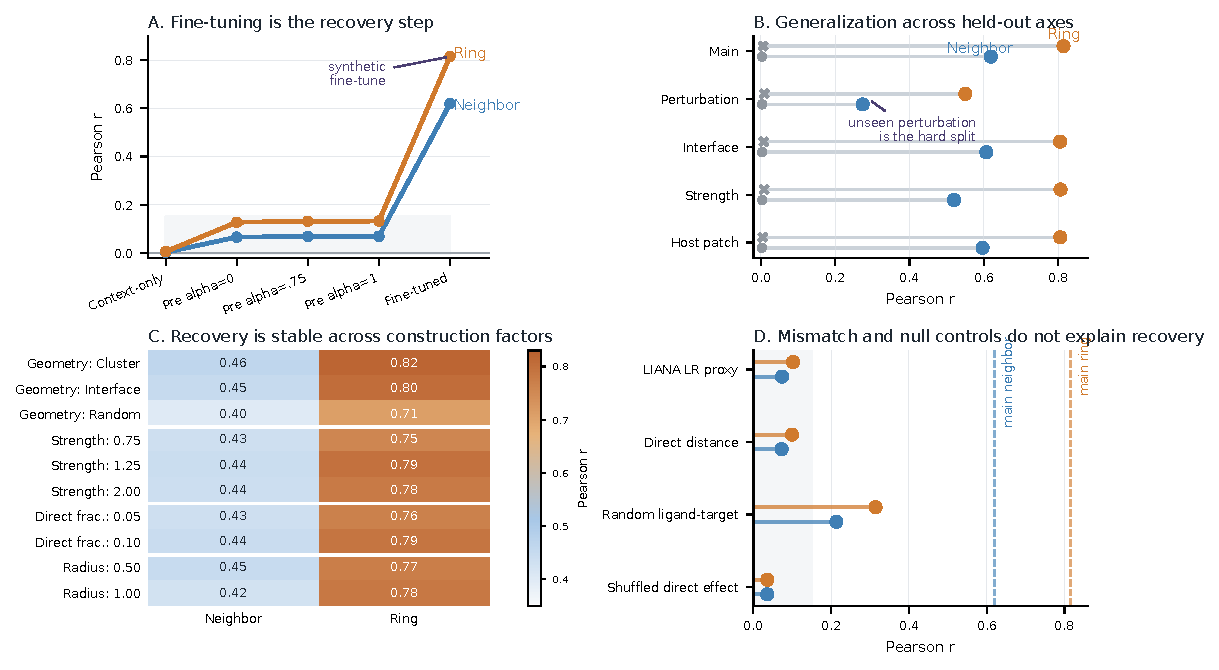
\includegraphics[width=\textwidth]{synthetic_lr_summary.pdf}
    \caption{\textbf{Controlled synthetic LR-propagation validation.}
    (A) Main-split model trajectory showing that direct transfer from the real-data
    pretrained model is weak, whereas synthetic fine-tuning recovers neighbor and
    ring-level structure. (B) Cross-split recovery from the niche-module-only baseline
    to the synthetic-trained model across held-out perturbation, interface geometry,
    strength, and host-patch splits. (C) Heatmap summary of trained recovery across
    geometry, strength, direct-effect fraction, and radius-scale factors. (D)
    Simulator mismatch and null-control settings remain far below the matched
    synthetic LR benchmark.}
    \label{fig:synthetic_lr_summary}
\end{figure*}

\begin{figure}[t]
    \centering
    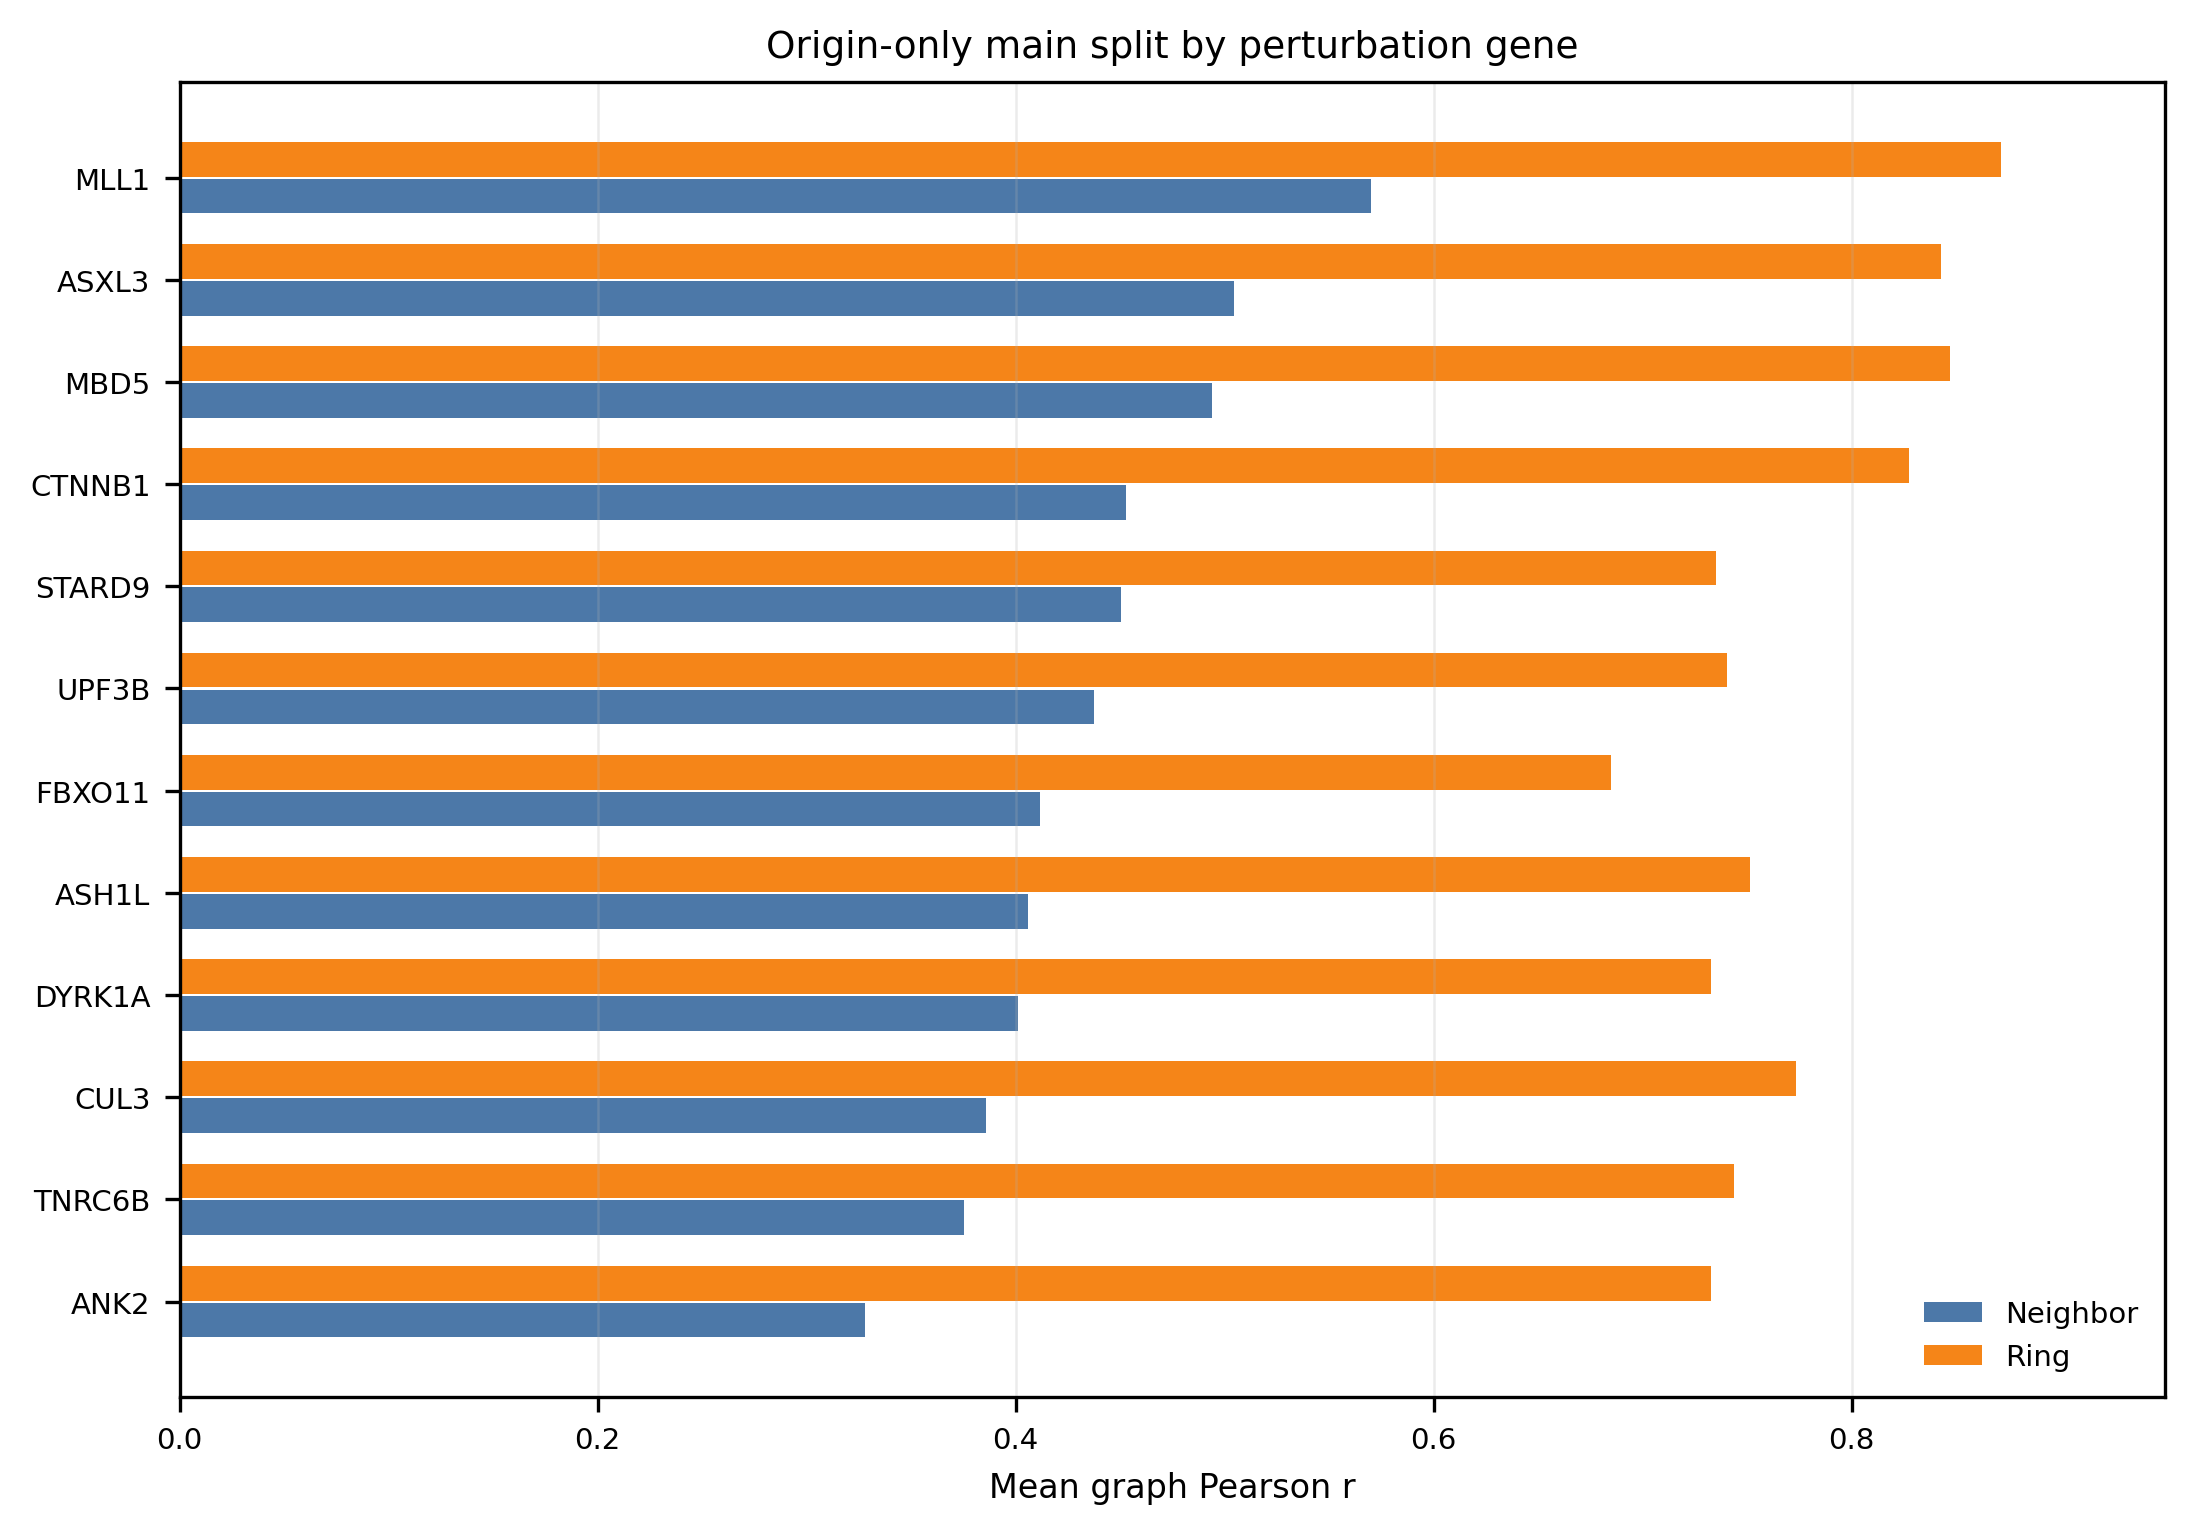
\includegraphics[width=0.9\linewidth]{synthetic_lr_gene_breakdown.png}
    \caption{\textbf{Main-split synthetic benchmark by perturbation gene.}
    Bars show mean graph Pearson $r$ for neighbor and ring-level recovery,
    ranked by perturbation gene. Ring-level recovery remains strong across perturbation
    genes, while neighbor recovery varies more across perturbation identities.}
    \label{fig:synthetic_lr_gene_breakdown}
\end{figure}

\begin{table}[t]
\centering
\small
\setlength{\tabcolsep}{4pt}
\renewcommand{\arraystretch}{1.08}
\caption{\textbf{Main model comparison on the controlled synthetic LR-propagation benchmark.}
Synthetic fine-tuning substantially improves neighbor and ring-level recovery
relative to niche-module-only prediction and direct transfer from the real-data pretrained model.}
\label{tab:synthetic_lr_main_models}
\begin{tabular}{lcccccc}
\toprule
Model & Neighbor & Centered & Ring & Center & $\Delta$Nei.\\
\midrule
Niche module only & 0.0033 & 0.0012 & 0.0062 & -0.0047 & 0.0000 \\
Pretrained, $\alpha=0$ & 0.0663 & 0.0087 & 0.1281 & 0.5003 & 0.0631 \\
Pretrained, $\alpha=0.75$ & 0.0692 & 0.0097 & 0.1320 & 0.5008 & 0.0659 \\
Pretrained, $\alpha=1$ & 0.0699 & 0.0101 & 0.1327 & 0.5003 & 0.0666 \\
Synthetic fine-tuned & \textbf{0.6193} & \textbf{0.3142} & \textbf{0.8148} & \textbf{0.9971} & \textbf{0.6160}\\
\bottomrule
\end{tabular}
\end{table}

\begin{table*}[t]
\centering
\small
\setlength{\tabcolsep}{4pt}
\renewcommand{\arraystretch}{1.08}
\caption{\textbf{Cross-split robustness on the controlled synthetic LR benchmark.}
The synthetic-trained model generalizes across held-out interface geometry, held-out
strength, and held-out host-patch splits. The held-out perturbation split is more
challenging but remains non-trivial relative to the near-zero niche-module-only baseline.}
\label{tab:synthetic_lr_cross_split}
\begin{tabular}{lccccccccc}
\toprule
Split & Train & Val & Test & Niche nei. & Niche ring & Trained nei. & Centered & Trained ring & Gain nei. / ring \\
\midrule
Main stratified & 252 & 72 & 108 & 0.0033 & 0.0062 & 0.6193 & 0.3142 & 0.8148 & 0.6160 / 0.8086 \\
Held-out perturbation & 252 & 72 & 108 & 0.0037 & 0.0095 & 0.2743 & 0.1842 & 0.5503 & 0.2706 / 0.5408 \\
Held-out interface & 240 & 48 & 144 & 0.0038 & 0.0076 & 0.6070 & 0.3207 & 0.8056 & 0.6032 / 0.7981 \\
Held-out strength $2.0$ & 240 & 48 & 144 & 0.0040 & 0.0089 & 0.5201 & 0.2273 & 0.8068 & 0.5161 / 0.7979 \\
Held-out host patch & 252 & 72 & 108 & 0.0030 & 0.0056 & 0.5970 & 0.2269 & 0.8063 & 0.5940 / 0.8006 \\
\bottomrule
\end{tabular}
\end{table*}




\begin{table}[t]
\centering
\scriptsize
\setlength{\tabcolsep}{2.5pt}
\renewcommand{\arraystretch}{1.05}
\caption{\textbf{Simulator mismatch and null controls.}
The trained model transfers weakly to mismatched or null simulators, supporting the
interpretation that the main synthetic benchmark tests a specific LR-propagation
distribution rather than generic target leakage.}
\label{tab:synthetic_lr_mismatch_null}
\resizebox{\columnwidth}{!}{%
\begin{tabular}{@{}lcccc@{}}
\toprule
Simulator &
\shortstack{$n$\\graphs} &
\shortstack{Trained\\nei.} &
\shortstack{Trained\\ring} &
\shortstack{Gain\\nei. / ring} \\
\midrule
Direct distance          & 360 & 0.0727 & 0.0994 & 0.0700 / 0.0948 \\
LIANA LR proxy           & 360 & 0.0739 & 0.1022 & 0.0715 / 0.0989 \\
Random ligand--target    & 360 & 0.2135 & 0.3144 & 0.2120 / 0.3141 \\
Shuffled direct effect   & 360 & 0.0357 & 0.0359 & 0.0332 / 0.0312 \\
\bottomrule
\end{tabular}%
}
\end{table}




\begin{table*}[t]
\centering
\small
\setlength{\tabcolsep}{4pt}
\renewcommand{\arraystretch}{1.08}
\caption{\textbf{Main-split breakdown by geometry, strength, direct-effect fraction, and radius scale.}
Niche-module-only predictions remain near zero across construction factors. Synthetic fine-tuning
recovers strong ring-level structure across all tested settings.}
\label{tab:synthetic_lr_factor_breakdown}
\begin{tabular}{llcccccc}
\toprule
Factor & Setting / model & $n$ & Neighbor & Nei. SEM & Centered & Ring & Ring SEM \\
\midrule
\multicolumn{8}{l}{\textit{Geometry strategy}} \\
Cluster, niche-only & -- & 36 & 0.0077 & 0.0014 & 0.0023 & 0.0158 & 0.0035 \\
Interface, niche-only & -- & 36 & 0.0044 & 0.0010 & 0.0009 & 0.0150 & 0.0035 \\
Random, niche-only & -- & 36 & 0.0063 & 0.0014 & 0.0016 & 0.0166 & 0.0030 \\
Cluster, trained & -- & 36 & 0.4608 & 0.0164 & 0.3755 & 0.8159 & 0.0098 \\
Interface, trained & -- & 36 & 0.4491 & 0.0148 & 0.3556 & 0.8011 & 0.0136 \\
Random, trained & -- & 36 & 0.3975 & 0.0174 & 0.2993 & 0.7069 & 0.0228 \\
\midrule
\multicolumn{8}{l}{\textit{Perturbation strength}} \\
0.75, niche-only & -- & 36 & 0.0068 & 0.0013 & 0.0015 & 0.0160 & 0.0029 \\
1.25, niche-only & -- & 36 & 0.0047 & 0.0012 & 0.0008 & 0.0147 & 0.0033 \\
2.00, niche-only & -- & 36 & 0.0069 & 0.0014 & 0.0025 & 0.0167 & 0.0037 \\
0.75, trained & -- & 36 & 0.4323 & 0.0153 & 0.3444 & 0.7538 & 0.0201 \\
1.25, trained & -- & 36 & 0.4391 & 0.0143 & 0.3439 & 0.7931 & 0.0118 \\
2.00, trained & -- & 36 & 0.4359 & 0.0204 & 0.3421 & 0.7769 & 0.0208 \\
\midrule
\multicolumn{8}{l}{\textit{Direct-effect fraction}} \\
0.05, niche-only & -- & 54 & 0.0064 & 0.0011 & 0.0016 & 0.0163 & 0.0025 \\
0.10, niche-only & -- & 54 & 0.0058 & 0.0010 & 0.0016 & 0.0153 & 0.0029 \\
0.05, trained & -- & 54 & 0.4309 & 0.0127 & 0.3464 & 0.7638 & 0.0139 \\
0.10, trained & -- & 54 & 0.4407 & 0.0146 & 0.3405 & 0.7854 & 0.0156 \\
\midrule
\multicolumn{8}{l}{\textit{Radius scale}} \\
0.50, niche-only & -- & 54 & 0.0059 & 0.0008 & 0.0017 & 0.0167 & 0.0024 \\
1.00, niche-only & -- & 54 & 0.0063 & 0.0012 & 0.0015 & 0.0149 & 0.0030 \\
0.50, trained & -- & 54 & 0.4470 & 0.0145 & 0.3915 & 0.7687 & 0.0158 \\
1.00, trained & -- & 54 & 0.4246 & 0.0127 & 0.2955 & 0.7806 & 0.0137 \\
\bottomrule
\end{tabular}
\end{table*}

\begin{table}[t]
\centering
\small
\setlength{\tabcolsep}{5pt}
\renewcommand{\arraystretch}{1.08}
\caption{\textbf{Synthetic benchmark by perturbation gene on the main split.}
Perturbation genes are ranked by neighbor Pearson.}
\label{tab:synthetic_lr_gene_breakdown}
\begin{tabular}{lcccc}
\toprule
Perturbation gene & $n$ graphs & Neighbor & Centered & Ring \\
\midrule
\textit{MLL1} & 11 & 0.5699 & 0.4459 & 0.8713 \\
\textit{ASXL3} & 7 & 0.5046 & 0.4149 & 0.8429 \\
\textit{MBD5} & 7 & 0.4938 & 0.4248 & 0.8471 \\
\textit{CTNNB1} & 9 & 0.4529 & 0.3684 & 0.8274 \\
\textit{STARD9} & 12 & 0.4503 & 0.3751 & 0.7349 \\
\textit{UPF3B} & 12 & 0.4373 & 0.3812 & 0.7404 \\
\textit{FBXO11} & 3 & 0.4117 & 0.3436 & 0.6850 \\
\textit{ASH1L} & 8 & 0.4061 & 0.3418 & 0.7513 \\
\textit{DYRK1A} & 13 & 0.4013 & 0.2635 & 0.7329 \\
\textit{CUL3} & 9 & 0.3857 & 0.3115 & 0.7737 \\
\textit{TNRC6B} & 7 & 0.3751 & 0.3115 & 0.7440 \\
\textit{ANK2} & 10 & 0.3279 & 0.1748 & 0.7328 \\
\bottomrule
\end{tabular}
\end{table}

\paragraph{Interpretation.}
The controlled synthetic benchmark supports three conclusions. First, niche-module-only
prediction remains near zero, so the synthetic response field is not recoverable from
tissue context alone. Second, synthetic fine-tuning generalizes well across held-out
graphs and construction factors, especially geometry, strength, direct-effect fraction, and
radius scale. Third, the held-out perturbation split is substantially harder than the
main stratified split, indicating that unseen perturbation identity remains the main
synthetic generalization bottleneck. We therefore use this benchmark as controlled
validation of direct-effect-conditioned propagation under known LR simulation rules, not as
a replacement for the real cell-resolved Spatial Perturb-Seq benchmark.

\subsection{Spot- and lesion-level external validation on Perturb-map / GSE193460}
\label{app:perturbmap_validation}

Perturb-map / GSE193460 provides a real spatial CRISPR validation setting with
spot- or lesion-level perturbation readouts. Because it does not provide matched
cell-resolved neighbor-response targets, we do not use it as an exact benchmark.
Instead, we aggregate \methodname{} predictions to spot-level and lesion-level gene
programs and compare them with observed perturbation-associated spatial signatures.

\begin{table}[t]
\centering
\small
\setlength{\tabcolsep}{4pt}
\renewcommand{\arraystretch}{1.08}
\caption{\textbf{Perturb-map / GSE193460 external validation.}
Spot-level Pearson correlations compare predicted and observed program scores.
Lesion-level Spearman correlations compare lesion-level ranking of perturbation-associated
programs.}
\label{tab:perturbmap_external}
\begin{tabular}{lcc}
\toprule
Readout & Spot Pearson $r$ & Lesion Spearman $\rho$ \\
\midrule
\textit{Ifngr2} top-25 program & 0.8528 & 0.5357 \\
\textit{Jak2} top-25 program & 0.7569 & 0.9286 \\
\textit{Tgfbr2} top-25 program & 0.7138 & 0.6071 \\
Curated TGF$\beta$--stroma program & 0.8076 & 0.7500 \\
IFN-response program & 0.6275 & -- \\
\bottomrule
\end{tabular}
\end{table}

\begin{table}[t]
\centering
\small
\setlength{\tabcolsep}{5pt}
\renewcommand{\arraystretch}{1.08}
\caption{\textbf{Top-$k$ sensitivity for Perturb-map spot-level validation.}
Top-50 equals top-25 because the common-gene mask does not add additional usable
genes beyond the top-25 set.}
\label{tab:perturbmap_topk}
\begin{tabular}{lccc}
\toprule
Signature & Top-10 & Top-25 & Top-50 \\
\midrule
\textit{Ifngr2} spot Pearson & 0.8252 & 0.8528 & 0.8528 \\
\textit{Jak2} spot Pearson & 0.7063 & 0.7569 & 0.7569 \\
\textit{Tgfbr2} spot Pearson & 0.6292 & 0.7138 & 0.7138 \\
\bottomrule
\end{tabular}
\end{table}



\begin{table}[t]
\centering
\small
\setlength{\tabcolsep}{2.2pt}
\renewcommand{\arraystretch}{1.06}
\caption{\textbf{Perturb-map bootstrap CIs and null controls.}
Spot-level programs are significant against score-permutation nulls
($p=0.001$); random gene-program nulls support selected readouts.}
\label{tab:perturbmap_null_ci}
\begin{tabularx}{\columnwidth}{@{}
>{\raggedright\arraybackslash}X
ccc@{}}
\toprule
Readout & Score & 95\% CI & \shortstack{Null\\$p$} \\
\midrule
\textit{Ifngr2} top-25 spot $r$      & 0.8528 & [0.8114, 0.8867] & 0.0150 \\
\textit{Jak2} top-25 spot $r$        & 0.7569 & [0.7019, 0.8014] & trend \\
\textit{Tgfbr2} top-25 spot $r$      & 0.7138 & [0.6647, 0.7545] & trend \\
TGF$\beta$--stroma spot $r$          & 0.8076 & [0.7648, 0.8423] & 0.0040 \\
\textit{Jak2} lesion $\rho$          & 0.9286 & --               & 0.0490 \\
\bottomrule
\end{tabularx}
\end{table}




\paragraph{Interpretation.}
Perturb-map provides a coarse external validation setting rather than a matched
cell-resolved propagation benchmark. The spot-level correlations are high and stable
under bootstrap resampling, and the top-$k$ sensitivity analysis shows that the
program-level agreement is not specific to a single top-$k$ threshold. Score-permutation
nulls are significant for all interpretable programs, while the stricter random
gene-program null supports the curated TGF$\beta$--stroma program, the \textit{Ifngr2}
top-25 spot program, and the \textit{Jak2} lesion-level ranking. These results support
cross-assay alignment of \methodname{} response fields under coarser Perturb-map
supervision, while preserving the primary role of Spatial Perturb-Seq as the exact
cell-resolved benchmark.





\begin{table*}[t]
\centering
\caption{Complete system-level baseline comparison on the block-holdout Spatial Perturb-seq benchmark. Neighbor, neighbor-centered, high-confidence neighbor, and ring metrics are Pearson correlations; higher is better. MAE is lower better. The niche-only row quantifies context-explainable response, whereas the two final rows separate perturbation-conditioned propagation from ring refinement.}
\label{tab:app_full_baseline_comparison}
\footnotesize
\setlength{\tabcolsep}{3pt}
\renewcommand{\arraystretch}{1.12}
\begin{tabularx}{\textwidth}{@{}>{\raggedright\arraybackslash}p{0.11\textwidth}
>{\raggedright\arraybackslash}X
>{\raggedright\arraybackslash}p{0.16\textwidth}
ccccc@{}}
\toprule
Group & Method & Perturbation input & Neigh. & N-centered & High-conf. & Ring & MAE \\
\midrule
Trivial &
Zero-delta / no-change &
none &
0.00000 & 0.00000 & 0.00000 & 0.00000 & 0.45344 \\

Niche &
Niche module only &
none &
0.60963 & 0.64284 & 0.50900 & 0.40510 & 0.43926 \\

Statistical &
Training-set guide mean &
guide ID &
0.00923 & 0.00000 & 0.01080 & 0.02657 & 0.46429 \\

Statistical &
Guide $\times$ cell-type $\times$ ring mean &
guide ID, cell type, ring &
0.00714 & -0.00045 & 0.00825 & 0.01731 & 0.46752 \\

Retrieval &
Nearest matched training patch transfer &
matched patch &
0.00012 & -0.00104 & 0.00060 & 0.00960 & 0.61186 \\

Linear &
Elastic-net patch regression &
patch features &
0.56953 & 0.59375 & 0.56896 & 0.39101 & 0.42737 \\

Generic graph &
GAT / GraphSAGE patch model &
graph features &
0.54532 & 0.56623 & 0.54550 & 0.39668 & 0.46293 \\

Single-cell adapted &
Direct-effect predictor + distance diffusion &
predicted direct effect &
0.00616 & 0.00028 & 0.00664 & 0.01434 & 0.45912 \\

CCC adapted &
CCC-gated linear propagation &
fixed CCC &
-0.00191 & 0.00316 & -0.00224 & 0.00052 & 0.50968 \\

Ours &
Base direct-effect$\rightarrow$neighbor propagation &
measured direct effect &
0.68410 & 0.71701 & 0.68317 & 0.45204 & 0.40939 \\

\rowcolor{blue!7}
Ours &
\methodname{} final propagation blend &
measured direct effect + refinement &
0.68443 & 0.71566 & 0.68340 & 0.45722 & 0.40762 \\
\bottomrule
\end{tabularx}
\end{table*}

\begin{table*}[t]
\centering
\caption{Aggregate gene-delta metrics for the same real-data run reported in the main gene-centric evaluation.}
\label{tab:app_gene_delta_metrics}
\small
\setlength{\tabcolsep}{5pt}
\renewcommand{\arraystretch}{1.12}
\begin{tabular}{lccccccc}
\toprule
Aggregation & Pearson & Spearman & Cosine & $R^2$ & MAE & RMSE & Sign acc. \\
\midrule
Flat all node--gene pairs & 0.679 & 0.336 & 0.679 & 0.460 & 0.417 & 0.857 & 0.483 \\
Flat neighbor pairs & 0.670 & 0.336 & 0.669 & 0.448 & 0.419 & 0.860 & 0.489 \\
Per-cell mean, all nodes & 0.690 & --- & 0.687 & 0.446 & 0.417 & 0.839 & 0.483 \\
Per-cell mean, neighbor cells & 0.686 & --- & 0.683 & 0.440 & 0.419 & 0.843 & 0.489 \\
\bottomrule
\end{tabular}
\end{table*}

\begin{table*}[t]
\centering
\caption{Core structural ablations on the held-out local benchmark. Deltas are relative to the final propagation blend. The main paper reports the compact diagnostic summary; this table preserves the full structural-ablation values. Residualization is the dominant structural contribution; edge and direct-effect inputs provide smaller additional gains.}
\label{tab:app_core_structural_ablations}
\small
\setlength{\tabcolsep}{5pt}
\renewcommand{\arraystretch}{1.12}
\begin{tabularx}{\textwidth}{@{}>{\raggedright\arraybackslash}Xccccc@{}}
\toprule
Variant & Neighbor & Ring & MAE & $\Delta$Neighbor & $\Delta$Ring \\
\midrule
\rowcolor{cyan!10}
\methodname{} final propagation blend &
0.68443 & 0.45722 & 0.40762 & --- & --- \\

No niche-impact residualization &
0.16451 & 0.15320 & 0.69832 & $-0.51992$ & $-0.30402$ \\

No edge attributes &
0.60591 & 0.41819 & 0.43651 & $-0.07852$ & $-0.03903$ \\

No direct-effect input &
0.61405 & 0.44062 & 0.42917 & $-0.07038$ & $-0.01660$ \\
\bottomrule
\end{tabularx}
\end{table*}

\begin{table*}[t]
\centering
\small
\caption{\textbf{Formal frozen-test drug/perturbation selector audit.}
Relative spillover reduction is measured against target-only; higher is better.
Regret is measured against the observed-field oracle; lower is better.
``Random qualified'' samples from actions qualified by observed utility and is
therefore not a deployable method.}
\label{tab:app_selector_formal}
\setlength{\tabcolsep}{4.5pt}
\begin{tabular}{@{}lrrrrr@{}}
\toprule
Method & TQR & Spillover red. & Regret & Safe@1 & Safe@5 \\
\midrule
Target-only (MLP-context utility) & 0.6944 & 0.0000 & 0.4668 & 0.1111 & 0.1111 \\
Random observed-qualified & 1.0000 & $-0.0983$ & 0.3849 & 0.0000 & 0.0000 \\
Path2 aggregation & 0.6667 & $-0.1638$ & 0.4726 & 0.0278 & 0.3333 \\
Dual MLP-utility + SPINE-burden & 0.6667 & 0.1291 & 0.3434 & 0.1389 & 0.4167 \\
\textbf{Validation-selected consensus} & \textbf{0.6944} & \textbf{0.1200} &
\textbf{0.3424} & \textbf{0.1667} & \textbf{0.4167} \\
Nonlinear consensus sensitivity & 0.7222 & 0.1265 & 0.3318 & 0.1667 & 0.4167 \\
Observed utility/burden oracle & 1.0000 & 0.6058 & 0.0000 & 1.0000 & 1.0000 \\
\bottomrule
\end{tabular}
\end{table*}

\begin{table*}[t]
\centering
\small
\caption{Exploratory burden decomposition for the three post-hoc cases. Scores
are observed field summaries. Lower burden is better.}
\label{tab:app_selector_burden_decomposition}
\begin{tabular}{llrrrrr}
\toprule
Target & Role & Target score & Weighted burden & Far-field & Off-program & Undesired \\
\midrule
TGF-$\beta$/stroma near-down & target-only & 5.074 & 1.188 & 1.213 & 1.228 & 1.457 \\
TGF-$\beta$/stroma near-down & selector & 4.968 & 0.597 & 0.604 & 0.615 & 0.778 \\
Vascular stress near-down & target-only & 2.734 & 1.278 & 1.213 & 1.347 & 1.655 \\
Vascular stress near-down & selector & 2.729 & 0.965 & 0.892 & 1.024 & 1.380 \\
Myeloid activation far-up & target-only & 1.578 & 0.717 & 0.918 & 0.742 & 0.811 \\
Myeloid activation far-up & selector & 1.409 & 0.542 & 0.651 & 0.550 & 0.657 \\
\bottomrule
\end{tabular}
\end{table*}

\begin{table*}[t]
\centering
\small
\caption{\textbf{Observed chemical-response audits of the drug-selector
interface.} Actions are compound--dose--time conditions where dose and time
are available. Context and global TQR are median target-qualified rates for
context-specific and context-agnostic selection. Tahoe-100M uses a
prespecified 128/1,026-pseudobulk-shard subset, not the full raw collection.}
\label{tab:app_chemical_selector}
\setlength{\tabcolsep}{4.5pt}
\begin{tabular}{@{}lrrrrrr@{}}
\toprule
Assay & Actions & Contexts & Specs & Context TQR & Global TQR & Burden red. \\
\midrule
LINCS Phase II (GSE70138) & 11,039 & 30 & 18 & 1.000 & 0.567 & 0.0988 \\
LINCS Phase I (GSE92742) & 44,696 & 71 & 18 & 1.000 & 0.600 & 0.1230 \\
Tahoe-100M pseudobulk subset & 1,137 & 50 & 18 & 1.000 & 0.640 & 0.0550 \\
Sci-Plex (GSE139944) & 151 & 2 & 18 & 1.000 & 1.000 & 0.0119 \\
\bottomrule
\end{tabular}
\vspace{6pt}

\begin{minipage}[t]{0.47\textwidth}
\raggedright\footnotesize
\textit{Confirmatory selector.}
\Cref{tab:app_selector_formal} uses 3,107 actions and 36 target specifications
from disjoint train, validation, and frozen-test blocks. Validation fixes the
utility source, burden score, and five-candidate operating point. On test, the
selected rule matches target-only TQR at 0.6944, reduces mean spillover by
0.1200, and lowers absolute burden by 0.1244 (95\% CI,
0.0559--0.1926). Burden decreases for 24 specifications, increases for seven,
and is unchanged for five. The 0.6058 oracle reduction shows that substantial
ranking headroom remains; the evidence supports a moderate target-retaining
effect rather than the larger development estimate.
\end{minipage}
\hfill
\begin{minipage}[t]{0.47\textwidth}
\raggedright\footnotesize
\textit{Exploratory and external scope.}
\Cref{tab:app_selector_burden_decomposition} decomposes three post-hoc cases
into far-field, off-program, and undesirable-program terms. These cases explain
the decision mechanism but do not estimate the formal effect because their
operating family was explored during development.
\Cref{tab:app_chemical_selector} instead uses observed response profiles to ask
whether context-specific drug--dose--time choices exhibit the same
utility--burden structure. LINCS Phase I/II provide the largest action pools;
Tahoe-100M pseudobulk and Sci-Plex provide single-cell-derived support. These
audits validate the decision formulation, not end-to-end spatial drug
prediction, treatment efficacy, or clinical safety.
\end{minipage}
\end{table*}

\FloatBarrier
\subsection{Single-column supporting diagnostics}
\label{app:single_column_diagnostics}
The remaining tables are intentionally single-column. They document parameter
sensitivity, seed and architecture controls, case-study readouts, external
module support, unseen-guide stress tests, and calibration. This order keeps
related narrow tables in the two available columns while the surrounding text
states the split, estimand, and claim boundary for each result.

\subsection{Propagation-blend sensitivity and reference-ST diagnostics}
\label{app:blend_and_reference_diagnostics}

\begin{table}[t]
\centering
\caption{Propagation-blend sensitivity on the held-out local benchmark. $\alpha=0$ is the base propagation module, and $\alpha=1$ is the reference-ST ring-refinement module.}
\label{tab:app_blend_sweep}
\small
\setlength{\tabcolsep}{5pt}
\renewcommand{\arraystretch}{1.10}
\begin{tabular}{cccccc}
\toprule
$\alpha$ & Neighbor & Neighbor-centered & Ring & Neighbor MAE & Score \\
\midrule
0.00 & 0.68410 & 0.71701 & 0.45204 & 0.40939 & 1.92869 \\
0.50 & 0.68467 & 0.71620 & 0.45667 & 0.40761 & 1.93692 \\
0.60 & 0.68453 & 0.71585 & 0.45708 & 0.40759 & 1.93733 \\
0.65 & 0.68443 & 0.71566 & 0.45722 & 0.40762 & \textbf{1.93737} \\
0.70 & 0.68430 & 0.71545 & 0.45731 & 0.40769 & 1.93730 \\
1.00 & 0.68309 & 0.71384 & 0.45681 & 0.40865 & 1.93438 \\
\bottomrule
\end{tabular}
\end{table}

The selected blend $\alpha=0.65$ gives the highest composite score in this sweep. The base propagation module is slightly stronger in neighbor-centered Pearson, while the reference-ST refinement improves ring structure.

\begin{table}[t]
\centering
\caption{Held-out diagnostics for the reference-ST microenvironment encoder. These metrics evaluate self-supervised pretraining objectives, not perturbation-response accuracy.}
\label{tab:app_organ_prior}
\small
\setlength{\tabcolsep}{8pt}
\renewcommand{\arraystretch}{1.12}
\begin{tabular}{lc}
\toprule
Diagnostic & Value \\
\midrule
Masked node-program loss & 1.13407 \\
Neighborhood-program loss & 0.45550 \\
Patch cell-type histogram loss & 0.01061 \\
Edge-prior loss & $3.8\times10^{-5}$ \\
Edge-prior correlation & 0.99439 \\
\bottomrule
\end{tabular}
\end{table}

The frozen reference encoder is trained only on unperturbed reference ST. These diagnostics verify that it learns stable microenvironment and edge-plausibility structure, but they should not be interpreted as perturbation-response accuracy.

\subsection{Confirmatory Direct-Effect Input Controls}
\label{app:profile_controls}

\begin{table}[t]
\centering
\caption{\textbf{B. Detailed direct-effect input controls.}
The factorial separates direct-effect profile identity, sender location, and
the cached communication prior.}
\label{tab:app_profile_controls}
\vspace{2pt}
\footnotesize
\setlength{\tabcolsep}{3pt}
\renewcommand{\arraystretch}{1.08}
\begin{tabular*}{\columnwidth}{@{\extracolsep{\fill}}lr@{}}
\toprule
Input control & Ring Pearson \\
\midrule
Correct profile + correct region & 0.4574 \\
Shuffled profile + correct region & 0.4056 \\
Correct profile + relocated region & 0.4314 \\
Random profile + random region & 0.4135 \\
Correct profile + randomized CCC & 0.4575 \\
\bottomrule
\end{tabular*}
\end{table}

The profile/location factorial shows that both molecular identity and sender
placement affect radial response organization, whereas randomizing cached CCC
scores does not.

\subsection{Development ablations}
\label{app:development_ablations}

The following tables retain the original development evidence but replace internal run names with compact labels. In \Cref{tab:app_ablation_modules}, rows marked ``block'' use the final spatial block-holdout setting, whereas rows marked ``coord'' come from earlier coordinate-split development runs. The early structural ablations show that explicit direct-effect-to-neighbor propagation is more effective than generic patch regression or purely semantic pairwise prediction. The recipe ablations show that longer optimization, three-control consensus targets, and post-state supervision improve earlier baselines, while strict same-type pseudo-pre targets are too noisy for the current local benchmark.

\begin{table}[t]
\centering
\caption{Broad module and structural ablations from development runs.}
\label{tab:app_ablation_modules}
\scriptsize
\setlength{\tabcolsep}{3pt}
\renewcommand{\arraystretch}{1.14}
\begin{tabular}{@{}lccc@{}}
\toprule
Variant & Direct & Neighbor & Ring \\
\midrule
Full structured, block & 0.959 & 0.670 & 0.421 \\
Niche only, block & 1.000 & 0.610 & 0.405 \\
Structured, coord & 0.963 & 0.643 & 0.375 \\
No post loss, coord & 0.963 & 0.640 & 0.373 \\
Semantic module, coord & 0.983 & 0.607 & 0.426 \\
Indicator only, coord & 0.188 & 0.486 & 0.342 \\
Pair-only diff., coord & 0.984 & 0.362 & 0.210 \\
\bottomrule
\end{tabular}
\end{table}

\begin{table}[t]
\centering
\caption{Training, target-construction, and split ablations.}
\label{tab:app_ablation_recipe}
\footnotesize
\setlength{\tabcolsep}{4pt}
\renewcommand{\arraystretch}{1.14}
\begin{tabularx}{\linewidth}{@{}>{\raggedright\arraybackslash}X>{\raggedright\arraybackslash}p{0.42\linewidth}@{}}
\toprule
Recipe change & Key metrics \\
\midrule
Single-control, 10$\rightarrow$30 epochs & neighbor $0.364\rightarrow0.509$; ring $0.236\rightarrow0.291$ \\
Single-control $\rightarrow$ consensus target & neighbor $0.364\rightarrow0.425$; ring $0.236\rightarrow0.279$ \\
Consensus, 10$\rightarrow$30 epochs & neighbor $0.425\rightarrow0.577$; ring $0.279\rightarrow0.355$ \\
Add post-state supervision & neighbor $0.425\rightarrow0.536$; ring $0.279\rightarrow0.361$ \\
Coordinate $\rightarrow$ block holdout & neighbor $0.643\rightarrow0.670$; ring $0.375\rightarrow0.421$ \\
Matched-control $\rightarrow$ strict pseudo-pre & neighbor $0.0028$; ring $0.0000$ \\
\bottomrule
\end{tabularx}
\end{table}

\subsection{Detailed structural and design-refinement ablations}
\label{app:structural_design_refinement}

\paragraph{Interpretation of structural ablations.}
The final propagation blend combines a shared niche-impact baseline with directed direct-effect-to-neighbor propagation and ring-aware refinement. Removing niche-impact residualization produces the largest collapse, indicating that directly predicting the response fails to separate background tissue variation from perturbation-conditioned propagation. Removing edge attributes reduces both neighbor and ring performance, showing that spatial geometry, cell-type-pair information, and communication-compatibility features improve propagation structure. Removing the direct-effect input also degrades neighbor prediction, especially beyond niche-module-only correlation, confirming that the propagation module benefits from a meaningful direct-effect signal.




\begin{table}[t]
\centering
\caption{Design-refinement ablations. Deltas are relative to the stated reference within each ablation family.}
\label{tab:app_design_refinement_ablations}
\small
\setlength{\tabcolsep}{1.6pt}
\renewcommand{\arraystretch}{1.05}
\begin{tabularx}{\linewidth}{@{}>{\raggedright\arraybackslash}Xrrr@{}}
\toprule
Ablation & $\Delta$Score & $\Delta$Neigh. & $\Delta$Ring \\
\midrule
Base propagation vs. niche only & --- & $+0.0745$ & $+0.0469$ \\
Base vs. ring refinement        & $-0.0057$ & $+0.0010$ & $-0.0048$ \\
Reference adapter only          & $-0.0018$ & $+0.0001$ & $-0.0013$ \\
Reference edge-prior gate       & $-0.0040$ & $-0.0006$ & $-0.0019$ \\
Plain second pass               & $-0.0008$ & $+0.0002$ & $-0.0007$ \\
No reference adapter            & $-0.0023$ & $+0.0011$ & $-0.0027$ \\
Include direct-cell loss        & $-0.0637$ & $-0.0131$ & $-0.0267$ \\
Remove ring loss                & $-0.0015$ & $+0.0002$ & $-0.0011$ \\
\bottomrule
\end{tabularx}
\end{table}





\paragraph{Interpretation of design-refinement ablations.}
These historical development ablations were run on the original comparison
split. They motivated the optional ring-aware refinement, but the new
randomized-CCC and reference-ST low-data diagnostics show no robust
communication-prior or reference-adapter gain. We therefore retain the
refinement only as an exact-task variant and do not treat either prior as a
core source of perturbation-conditioned signal. Including direct-effect-cell
reconstruction in the propagation loss substantially hurts receiver
prediction, indicating that the easier direct signal can dominate training.

\paragraph{Compact IFN-\texorpdfstring{$\gamma$}{gamma} readout summary.}
The de novo IFN-$\gamma$ example is interpreted as hypothesis generation, not matched validation. Its main qualitative pattern is a spatially extended IFN/MHC-I-like response: immune and vascular-associated states are enriched among high-response targets, canonical IFN/MHC-I genes increase, selected structural or vascular programs decrease, and patch-level gradients show that the response is spatially heterogeneous rather than a uniform slide-wide shift. The key numerical readouts are summarized below; the following text gives the biological interpretation.





\begin{table}[t]
\centering
\caption{Key numerical readouts for the de novo IFN-$\gamma$ case study.}
\label{tab:app_ifng_case_readouts}
\footnotesize
\setlength{\tabcolsep}{4pt}
\renewcommand{\arraystretch}{1.12}
\begin{tabularx}{\linewidth}{@{}>{\raggedright\arraybackslash}p{0.34\linewidth}>{\raggedright\arraybackslash}X@{}}
\toprule
Readout & Value \\
\midrule
Top-pathway target composition &
Microglia 11.91\% vs. 7.98\% background; endothelial 7.81\% vs. 7.22\%; pericyte 5.81\% vs. 5.49\%. \\

Canonical IFN/MHC-I genes &
\textit{B2m} $+1.91$, \textit{H2-D1} $+1.57$, \textit{Ifitm3} $+1.72$. \\

Suppressed programs &
\textit{Col1a2} $-1.31$, \textit{Vcan} $-1.28$, \textit{Flt1} $-1.82$. \\

Spatial field coverage &
2,048 top-5\% targets; 64NN union covers 38,922/40,944 bottom-right cells (95.06\%). \\

Context-dependent gradients &
Patch $x$ coordinate: \textit{B2m} $r=-0.290$, \textit{Irf8} $r=-0.296$, \textit{Col1a2} $r=+0.307$, \textit{Flt1} $r=+0.417$. \\

Representative local patches &
P1--P6 at $(14955,8981)$, $(18877,11976)$, $(15281,12090)$, $(14662,15755)$, $(19830,17042)$, and $(16754,18181)$. \\

Optional-adapter deployment context &
Adapter used in the displayed deployment; no matched IFN-$\gamma$ labels or
paired deployment ablation, so no architectural claim is made. \\
\bottomrule
\end{tabularx}
\end{table}






\subsection{Extended de novo IFN-\texorpdfstring{$\gamma$}{gamma} case-study interpretation}
\label{app:ifng_extended_interpretation}

\paragraph{External IFN-\texorpdfstring{$\gamma$}{gamma} direct-effect seed.}
The de novo IFN-$\gamma$ seed is generated from an external cytokine perturbation source rather than from the target ST slide. We train/fine-tune CPA on PerturbSapiens cytokine data with treatment status, cell type, and tissue/broad class as covariates. Treatment status distinguishes PBS/control and IFN-$\gamma$. For each Sample2/pre4 spatial cell, CPA is queried twice with the same cell and tissue covariates: once under the IFN-$\gamma$ condition and once under the PBS/control condition. The direct-effect seed is
\[
d_i^{\mathrm{IFN}\gamma}
=
\widehat{x}_{i}^{\mathrm{IFN}\gamma}
-
\widehat{x}_{i}^{\mathrm{PBS}} .
\]
The resulting per-cell direct delta is mapped to the benchmark gene set and used only as the direct-effect input for \methodname{} propagation. No paired IFN-$\gamma$ spatial perturbation label from the Sample2/pre4 tissue block is used during this inference.

\begin{table}[t]
\centering
\footnotesize
\setlength{\tabcolsep}{5pt}
\renewcommand{\arraystretch}{1.05}
\caption{Direct-effect seed construction for the de novo IFN-$\gamma$ mouse-brain case study.}
\label{tab:app_ifng_direct_effect_seed}
\begin{tabularx}{\linewidth}{lX}
\toprule
\textbf{Component} & \textbf{Specification} \\
\midrule
External perturbation source & PerturbSapiens cytokine data \\
Single-cell response model & CPA trained/fine-tuned on cytokine perturbation responses \\
Covariates & Treatment status, cell type, and tissue/broad class \\
Treatment contrast & IFN-$\gamma$ state minus PBS/control state \\
Spatial target cells & Sample2/pre4 mouse-brain spatial cells \\
Direct-effect seed &
\makecell[l]{Per-cell delta\\
\(\begin{aligned}
d_i^{\mathrm{IFN}\gamma}
&=\widehat{x}_{i}^{\mathrm{IFN}\gamma}\\
&\quad-\widehat{x}_{i}^{\mathrm{PBS}}
\end{aligned}\)} \\
Use in \methodname{} & Direct-effect input for spatial propagation; no paired IFN-$\gamma$ spatial labels are used \\
\bottomrule
\end{tabularx}
\end{table}

\paragraph{Spatial heterogeneity.}
The predicted response is not dominated by a single global offset. The whole-tissue maps identify regions with strong IFN-associated activation, while the local patch panels show that the signal extends into neighboring cells. Different genes show different response signs, and the same perturbation query produces region-dependent response magnitudes across selected patches.

\paragraph{Cell-state enrichment.}
The high-response regions are enriched for immune and glial-associated tissue context. Among top-pathway 5\% target cells, microglia account for 11.91\% of targets compared with a 7.98\% background frequency, corresponding to a 1.49$\times$ enrichment. Endothelial and pericyte states are mildly enriched as well, at 7.81\% versus 7.22\% and 5.81\% versus 5.49\%, respectively. This suggests that the de novo response field is concentrated in immune-, vascular-, and glial-associated niches rather than assigned uniformly across the tissue.

\paragraph{Gene-program response.}
At the gene-program level, the model predicts a coherent IFN-$\gamma$/MHC-I-like response. Target-cell deltas are positive for canonical interferon and antigen-presentation genes, including \textit{B2m} $(+1.91)$, \textit{H2-D1} $(+1.57)$, and \textit{Ifitm3} $(+1.72)$. In parallel, selected structural or vascular-associated programs are suppressed, including \textit{Col1a2} $(-1.31)$, \textit{Vcan} $(-1.28)$, and \textit{Flt1} $(-1.82)$. The selected local patches recapitulate this pattern at neighborhood scale: patch-averaged deltas are consistently positive for \textit{B2m} and \textit{Ifitm3}, and consistently negative for \textit{Col1a2} and \textit{Vcan}. Across the six displayed patches, \textit{B2m} averages range from $+0.69$ to $+0.96$, \textit{Ifitm3} from $+0.24$ to $+0.33$, while \textit{Col1a2} and \textit{Vcan} remain negative.

\paragraph{Extended spatial field.}
The predicted response forms an extended spatial field. The 64-nearest-neighbor union around 2,048 top-5\% targets covers 38,922 of 40,944 cells in the analyzed bottom-right region, or 95.06\%. Thus, the deployment output should be interpreted as a tissue-level response field rather than a set of isolated target-cell predictions. Consistent with this interpretation, patch-level spatial gradients show that the $x$ coordinate is negatively associated with \textit{B2m} response $(r=-0.290,\ p=4.2\times10^{-41})$ and \textit{Irf8} response $(r=-0.296,\ p=8.8\times10^{-43})$, and positively associated with \textit{Col1a2} response $(r=+0.307,\ p=5.7\times10^{-46})$ and \textit{Flt1} response $(r=+0.417,\ p=7.4\times10^{-87})$.

\paragraph{Role of the optional reference adapter.}
The displayed deployment used the frozen adapter, but no matched
IFN-$\gamma$ spatial labels or paired deployment ablation are available.
Low-data paired diagnostics show gains near zero, so this case cannot establish
that the adapter improves localization. It is a hypothesis-generating
interface example, not experimental validation of IFN-$\gamma$ biology or of
the reference adapter.

\subsection{Extended discussion}
\label{app:extended_discussion}

\paragraph{Controlled propagation versus de novo perturbation prediction.}
\methodname{} separates two problems that are often conflated in spatial perturbation modeling. The benchmark evaluates propagation conditioned on a direct-effect profile, while de novo use additionally requires a model that maps perturbation identity to that profile. This separation avoids attributing errors in direct-effect prediction to the spatial propagation module, and it makes the neighbor-response task directly measurable with Spatial Perturb-Seq supervision.

\paragraph{Role of niche-impact residualization.}
Matched-control construction, local anatomy, and cell-type composition explain a substantial fraction of the observed neighbor response field. A model that predicts the full delta directly can therefore obtain high flat neighbor correlation by fitting tissue context rather than perturbation-conditioned propagation. Niche-impact residualization reduces this shortcut: the niche module accounts for background tissue variation, and the propagation module is forced to explain direct-effect-driven response beyond that baseline.

\paragraph{Why ring lift matters.}
Flat Neighbor Pearson is not a sufficient diagnostic of perturbation conditioning, because several direct-effect perturbation controls retain high Neighbor Pearson through the niche module. Ring-level lift is more sensitive to whether perturbation information changes the radial organization of neighbor response. The measured direct-effect model produces the largest ring lift over niche-module-only prediction, whereas shuffled or noisy controls largely collapse back toward the niche-impact baseline.

\paragraph{Reference-ST diagnostic.}
The reference-ST encoder is pretrained from unperturbed spatial transcriptomics
and frozen before perturbation training. It supplies no perturbation-response
labels. Paired Ring gains are $+0.0009$, $+0.0002$, and $+0.0032$ at 10\%,
25\%, and 50\% paired-data fractions and approximately $+0.0005$ at full
data. These results do not support the adapter as a core component.

\paragraph{Interpretation of the IFN-$\gamma$ case study.}
The IFN-$\gamma$ analysis should be read as a hypothesis-generating deployment demonstration rather than a matched experimental validation. It shows that a perturbation-identity-derived direct-effect profile can produce spatially heterogeneous response fields, recover canonical IFN/MHC-I-like genes, suppress selected structural or vascular-like programs, and generate local response gradients. These outputs illustrate the intended deployment interface, but their biological claims require direct experimental validation.

\subsection{Extended Drug and Perturbation Selector Evaluation}
\label{app:selector_audit}

The selector treats target retention and burden ranking as separate prediction
problems. The formal audit uses 3,107 guide--site actions from spatially
disjoint train, validation, and frozen-test blocks (1,342/837/928 actions) and
36 target specifications. Predicted utility is supplied by the strict
context-only MLP aggregation; validation chooses the burden model and a
five-candidate operating point under a TQR constraint equal to validation
target-only. Neither the model family nor the threshold is adjusted after
opening the test block.

For the validation-selected selector, mean absolute burden decreases by 0.1244
with a target-specification bootstrap 95\% interval of [0.0559, 0.1926].
Relative reduction is 0.1200 with interval [$-0.0018$, 0.2289]; program-level
and program--Ring intervals are [0.0102, 0.2241] and
[$-0.0165$, 0.2400], respectively. The action selected by the frozen rule has
lower burden for 24 specifications, higher burden for seven, and unchanged
burden for five. These estimates support a moderate target-retaining benefit,
not the 25--35\% reduction hypothesized during development.

\begin{table}[t]
\centering
\scriptsize
\caption{\textbf{Pairwise lower-burden ranking on the formal test block.}
Confidence intervals are grouped bootstrap intervals over target
specifications and action pairs.}
\label{tab:app_selector_pairwise}
\setlength{\tabcolsep}{4pt}
\begin{tabular}{@{}lrr@{}}
\toprule
Burden score & Agreement & 95\% CI \\
\midrule
MLP context & 0.4909 & [0.4707, 0.5092] \\
MLP full & 0.5065 & [0.4907, 0.5223] \\
SPINE context aggregation & 0.5819 & [0.5651, 0.5989] \\
\textbf{SPINE context head} & \textbf{0.6250} & \textbf{[0.6108, 0.6393]} \\
SPINE full aggregation & 0.5811 & [0.5672, 0.5947] \\
SPINE full head & 0.5630 & [0.5495, 0.5763] \\
Context/full consensus ($w=0.25$) & 0.6183 & [0.6038, 0.6330] \\
\bottomrule
\end{tabular}
\end{table}

The context head provides the strongest standalone ranking signal, while the
validation-selected end-to-end consensus uses a more conservative utility and
burden combination. The gap between pairwise agreement and selected-action
benefit indicates that the remaining error is concentrated in target
qualification and extreme-rank calibration.

\paragraph{Exploratory case discovery.}
A separate development analysis scores target utility and three burden
components: far-field, off-program, and prespecified undesirable-program
responses. Across 5,286 candidate actions and 36 target specifications, its
operating points reached burden reductions of 0.354 and 0.418, while the
observed-field oracle reached 0.672. Because the legacy cache duplicated
training graphs in validation and the selector family was explored post hoc,
these values and the following cases are retained only as discovery evidence
and are not confirmatory effect estimates.

\begin{figure*}[t]
\centering
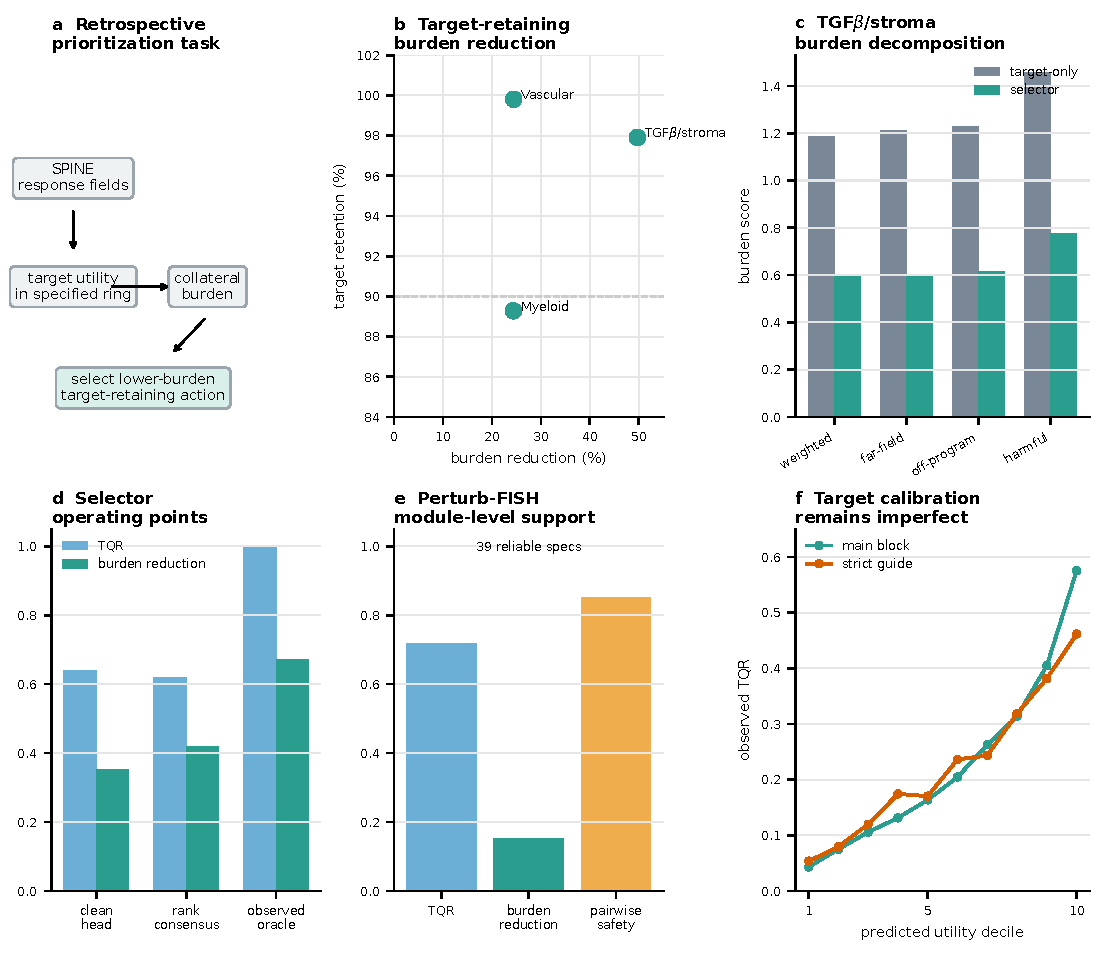
\includegraphics[width=\textwidth]{selector_prioritization_appendix.pdf}
\caption{\textbf{Exploratory post-hoc perturbation-prioritization audit.}
(a) Selector interface and audit scale: frozen \methodname{} response fields are decomposed into target utility and collateral burden and used to rank target-retaining, low-burden actions.
(b) Three exploratory biological cases show high target retention and lower collateral burden.
(c) Burden decomposition across all three cases shows weighted, far-field, off-program, and undesirable-program burden reductions.
(d) Spatial Perturb-seq operating points show the trade-off between target-qualified rate and burden reduction, with the observed-field oracle as an upper reference.
(e) Perturb-FISH provides module-level external support under a different action pool and readout panel.
(f) Predicted target utility stratifies observed target qualification, but absolute calibration remains incomplete under both main-block and strict-guide splits.}
\label{fig:app_selector_prioritization}
\end{figure*}

The three exploratory cases retained 89.3--99.8\% of target utility while
reducing collateral burden by 24.4--49.7\%
(Table~\ref{tab:app_selector_cases}). These cases illustrate the
utility--burden mechanism but were selected post hoc and are not used to
estimate the formal selector effect.

\begin{table}[t]
\centering
\scriptsize
\caption{Exploratory post-hoc response-field prioritization cases.}
\label{tab:app_selector_cases}
\setlength{\tabcolsep}{3pt}
\begin{tabular}{@{}lllrr@{}}
\toprule
Target & Target-only & Selector & Retain & Burden red. \\
\midrule
TGF$\beta$/stroma & \texttt{rraga} & \texttt{oligo2} & 97.9\% & 49.7\% \\
Vascular stress & \texttt{rraga} & \texttt{clu} & 99.8\% & 24.4\% \\
Myeloid activation & \texttt{Cfap410} & \texttt{stk39} & 89.3\% & 24.4\% \\
\bottomrule
\end{tabular}
\end{table}

\begin{table}[t]
\centering
\small
\caption{Exploratory selector operating points from the discovery analysis.}
\label{tab:app_selector_operating_points}
\setlength{\tabcolsep}{4pt}
\begin{tabular}{@{}lrrrr@{}}
\toprule
Operating point & Actions & Specs & TQR & Burden red. \\
\midrule
Clean weighted & 5,286 & 36 & 0.639 & 0.354 \\
Off-program & 5,286 & 36 & 0.667 & 0.362 \\
Rank-consensus & 5,286 & 36 & 0.620 & 0.418 \\
Observed oracle & 5,286 & 36 & 1.000 & 0.672 \\
\bottomrule
\end{tabular}
\end{table}

Perturb-FISH provides module-level external support rather than exact selector
replication because its action pool and readout panel differ from Spatial
Perturb-seq. On 39 reliable specifications, selection using predicted utility
and burden reached TQR 0.718 and burden reduction 0.151. Holding qualification
to observed utility and ranking by predicted burden increased the reduction to
0.207; pairwise burden-order agreement was 0.851
(Table~\ref{tab:app_selector_perturb_fish}). The spillover head also improves
median burden correlation from 0.539 for aggregation to 0.855 and reaches
Safe@5 of 1.0 on the reliable subset. Thus, the external assay strongly
supports burden ranking, while the observed-versus-predicted utility gap again
isolates target retention as the bottleneck.

\begin{table}[t]
\centering
\scriptsize
\caption{Perturb-FISH module-level support for the prioritization audit.}
\label{tab:app_selector_perturb_fish}
\setlength{\tabcolsep}{3pt}
\begin{tabular}{@{}lrrrrr@{}}
\toprule
Subset & Specs & TQR & Burden & Obs-U & Pairwise agreement \\
\midrule
Reliable specifications & 39 & 0.718 & 0.151 & 0.207 & 0.851 \\
All specifications & 64 & 0.641 & 0.137 & 0.218 & 0.851 \\
\bottomrule
\end{tabular}
\end{table}

\paragraph{Observed chemical-response selector audits.}
The generic action in Equation~\ref{eq:selector} can represent a
drug--dose--time intervention. We therefore applied the same frozen
target-module and harmful-module definitions to four public chemical-response
resources (Table~\ref{tab:app_chemical_selector}). These are
\emph{observed-response} audits: they test whether a context-aware,
target-retaining drug selector is a meaningful decision problem once response
profiles are available, rather than whether \methodname{} predicts those
non-spatial profiles.

LINCS Phase II contains 118,050 module-scored signatures and shows target and
harmful-burden rank-reversal rates of 0.917 and 0.868 across cell contexts.
The independent Phase I matrix contains 473,647 signatures and reproduces the
context-aware advantage over 44,696 actions. Tahoe-100M pseudobulk and
Sci-Plex provide single-cell-derived support, although their burden reductions
are smaller. ToxCast (8,597 chemicals, 617 endpoints) and Tox21 (7,831
chemicals, 12 endpoints) additionally show endpoint-dependent burden rankings,
with reversal rates of 0.443 and 0.191; because they lack a matched target
utility field, they support toxicity-endpoint heterogeneity but are not counted
as target-retaining selector validations.

\paragraph{Strict unseen-guide stress test.}
The selector is substantially less reliable when all test guides are unseen
(Table~\ref{tab:app_selector_guide_ood}). The predicted burden score remains
non-random (pairwise agreement 0.621; median burden Spearman 0.283), and the
observed oracle shows that a 0.350 reduction is available. However, the best
constrained predicted selector reaches only TQR 0.333 and reduction 0.068,
below the target-only TQR of 0.528. Removing the utility constraint recovers
reduction 0.288 but collapses TQR to 0.056. This decomposition identifies
unseen-guide target calibration, rather than absence of lower-burden actions,
as the failure mode.

\begin{table}[t]
\centering
\small
\caption{Strict guide-held-out selector stress test.}
\label{tab:app_selector_guide_ood}
\setlength{\tabcolsep}{4pt}
\begin{tabular}{@{}lrr@{}}
\toprule
Setting & TQR & Burden red. \\
\midrule
Target-only & 0.528 & 0.000 \\
Best constrained selector & 0.333 & 0.068 \\
No utility constraint & 0.056 & 0.288 \\
Observed utility/burden oracle & 1.000 & 0.350 \\
\bottomrule
\end{tabular}
\end{table}

Finally, predicted utility deciles stratify observed target qualification, but
absolute reliability remains incomplete: the main block split rises from TQR
0.043 to 0.575 across extreme deciles, while strict guide holdout rises from
0.053 to 0.461 (Table~\ref{tab:app_selector_calibration}). We therefore report
this as a retrospective drug/perturbation prioritization audit, not a calibrated
prospective controller or clinical safety predictor.

\begin{table}[t]
\centering
\small
\caption{Target-utility calibration limitation. Target-qualified rate (TQR) increases from the lowest to highest predicted-utility decile, but absolute calibration remains incomplete, especially under strict guide holdout.}
\label{tab:app_selector_calibration}
\begin{tabular}{lrrr}
\toprule
Split & Bottom-decile TQR & Top-decile TQR & Gap \\
\midrule
Main block & 0.043 & 0.575 & 0.532 \\
Strict guide & 0.053 & 0.461 & 0.408 \\
\bottomrule
\end{tabular}
\end{table}
\FloatBarrier

\subsection{Whole-block visualization wrapper}
\label{app:whole_block_wrapper}

The quantitative benchmark is local and matched-control based. For whole-block visualization, we keep the same trained local model but change only the inference layout. Predictions are first generated in matched-control patch coordinates, then softly projected onto the post-perturbation layout using same-cell-type, relative-position, and expression-similarity correspondence. Patch predictions are merged by post anchors rather than control donor rows, preventing control-patch deduplication from collapsing spatial coverage. This wrapper is used for visualization and external-study deployment; it is not mixed with the local paired-patch metrics.


\subsection{Experiment compute resources}
\label{app:compute_resources}

All experiments were run on a Linux workstation with NVIDIA RTX A6000 GPUs. Each GPU has 48 GB memory. The reference machine had 8 GPUs available, but each released training or evaluation command uses a single GPU by default through \texttt{--device cuda}. The machine had 64 logical CPU threads and 1 TB system RAM. CPU and storage throughput mainly affect raw-data preprocessing and graph construction; model training uses compact fixed-size graph patches.

Unless otherwise stated, \methodname{} experiments use 64-cell graph patches. The released scripts expose all compute-relevant settings, including batch size, epoch count, learning rate, device flag, split setting, and random seed.

\paragraph{Main \methodname{} experiment.}
Dataset construction uses patch size 64, a spatial-block split, training blocks \texttt{top\_right} and \texttt{bottom\_left}, test block \texttt{bottom\_right}, consensus target aggregation, and 3 matched controls per anchor. The niche module uses hidden dimension 256, 3 encoder layers, 3 propagation layers, batch size 16, 30 epochs, and learning rate $3\times10^{-4}$. The residual direct-effect-to-neighbor model uses hidden dimension 256, 3 propagation layers, batch size 16, 10 epochs, and learning rate $3\times10^{-4}$.

The reference-ST niche prior model uses patch size 64, edge $k=8$, local CCC top-$k=5$, 4096/512/512 train/validation/test samples, hidden dimension 128, batch size 32, 20 epochs, and learning rate $10^{-3}$. The organ-ring refinement uses batch size 16: the organ-adapter stage runs for 10 epochs at $5\times10^{-4}$, the response-refine stage for 6 epochs at $2\times10^{-4}$, the ring-refine stage for 6 epochs at $10^{-4}$, and the final organ-ring stage for 6 epochs at $7.5\times10^{-5}$. Best-model evaluation uses batch size 16 and sweeps $\alpha\in\{0.0,0.25,0.5,0.55,0.6,0.65,0.7,0.75,1.0\}$.

\paragraph{Ablations and baselines.}
OrganRingBlend ablations use the same residual graph model with hidden dimension 256, 3 propagation layers, batch size 16, and 6--10 epochs depending on the ablation. Seed and shortcut controls use batch size 16 and random seed 0. The shallow MLP baseline uses hidden dimension 512, batch size 8192, 20 epochs, and learning rate $10^{-3}$. Source/radial and summary baselines are CPU-light evaluation jobs.

\paragraph{Validation experiments.}
For Perturb-map / GSE193460, pseudo-ground-truth construction uses 64-cell patches and CPU preprocessing. Leave-one-out fine-tuning uses batch size 4, 80 epochs, learning rate $3\times10^{-4}$, and weight decay $10^{-4}$. Masked external evaluation and program validation use batch size 4. Robustness analysis uses 1000 null trials.

For GSE157977 synthetic ligand--receptor validation, direct-profile construction and gene-space projection are CPU preprocessing steps. Synthetic graph construction uses random seed 0. Direct-effect ablation evaluation uses batch size 16 and GPU evaluation.

For Perturb-FISH validation, graph construction uses 64-cell patches, at most 25 centers per perturbation, at least 5 positive cells, and random seed 11. The native ridge effect model uses $\alpha\in\{0.01,0.1,1,10,100,1000\}$ and 1000 null trials. The native \methodname{} graph model uses hidden dimension 256, 3 propagation layers, batch size 16, 30 epochs, learning rate $3\times10^{-4}$, weight decay $10^{-4}$, and patience 8.

\paragraph{Optional foundation-adapter experiments.}
CellPLM embedding construction uses batch size 512 and \texttt{cuda:0}. scGPT embedding construction uses batch size 32 and \texttt{cuda:0}. Frozen expression+niche adapters use CPU feature construction followed by the same \methodname{} residual training settings described above.

Exact wall-clock time depends on GPU model, CPU memory, and storage throughput. The released code package specifies the hardware class and all per-experiment compute settings needed to reproduce the reported experiments.





\end{document}
